\section{Mètodes Factorials}


\subsection{Anàlisi de Correspondències Múltiples}

Per tal d'indagar una mica més a la nostra base de dades i aprofitar les variables que podem extreure per l'entrenament de la xarxa neuronal, es durà a terme una Anàlisi de Correspondències Múltiple (ACM). Per culpa de la gran quantitat de variables categòriques, i sobretot, al gran nombre de modalitats que tenim en varies de les variables, sabem que la projecció que maximitzi la variància expressada per les diferents variables no seria prou prometedora.

Així doncs, predient la baixa variància explicada per la projecció, hem decidit excloure aquelles variables amb gran quantitat de modalitats, com totes les temporals, noms de cançons o noms d'artistes. En total, s'han fet servir les següents variables categòriques: \textit{album\_type}, \textit{key}, \textit{time\_signature},\textit{ rank\_group}, \textit{nationality}, \textit{gender},\textit{ is\_group}, \textit{pop}, \textit{hip\_hop}, \textit{rock}, \textit{electro}, \textit{christmas}, \textit{cinema}, \textit{latino}, \textit{collab} i \textit{major\_mode}. En fer l'ACM amb aquestes variables, trobem massa modalitats a la variable \textit{nationality}, cosa que complica una mica la visualització de les diferents projeccions de les modalitats i baixa molt la explicabilitat de cadascun dels eixos, tal i com es pot visualitzar a la figura \ref{fig:ACM1_varianciaDimensions}. Així i tot, s'intentarà fer l'anàlisi amb aquesta variable inclosa, ja que algunes d'aquestes modalitats sí que tenen valor significatiu, implicant informació valuosa a l'hora d'entrenar la xarxa.

\begin{figure}[H]
    \centering
    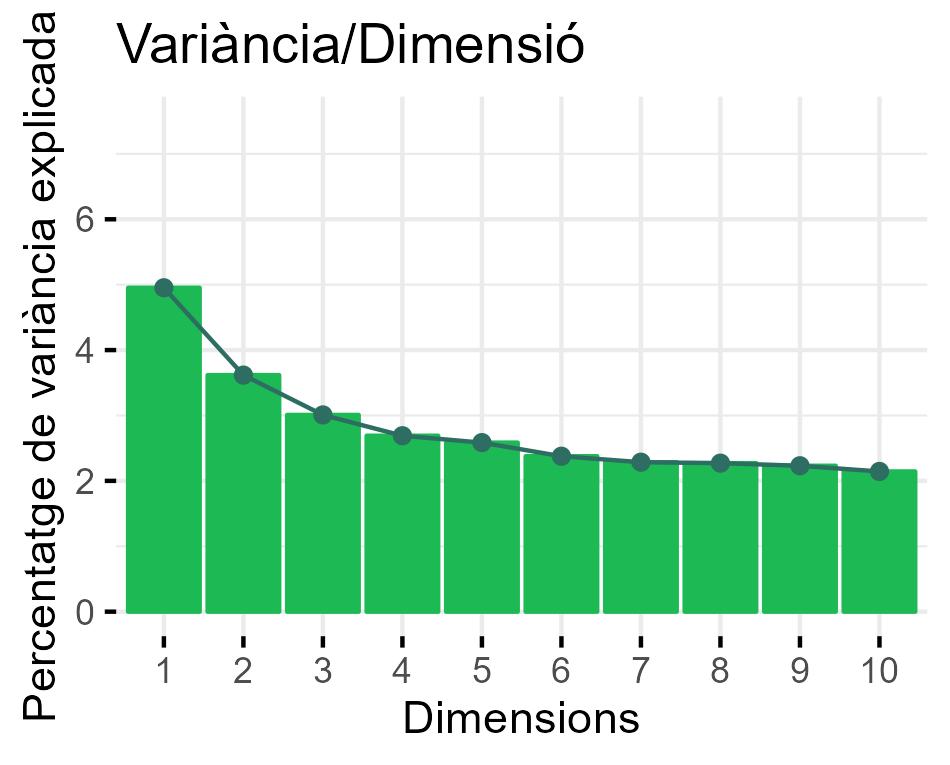
\includegraphics[width=0.5\linewidth]{Images/6_Factorial_Methods/ACM/ACM1_varianciaDimensions.png}
    \caption{Variància aportada per les primeres 10 dimensions amb més explicabilitat del \textit{ACM}}
    \label{fig:ACM1_varianciaDimensions}
\end{figure}

Tal com es pot veure a la figura \ref{fig:ACM1_contribVars1}, les modalitats els gèneres tenen una gran contribució al primer eix (sobretot \textit{latino}, \textit{pop}, \textit{hip\_hop} i \textit{electro}), junt amb algunes nacionalitats com Puerto Rico, Colòmbia o UK. Destacar també la lleugera importància que tenen el gènere femení, masculí i \textit{mixed} en aquest primer eix. En la figura \ref{fig:ACM1_contribVars2}, en canvi, observem com altres gèneres musicals (\textit{rock}, \textit{christmas} i \textit{pop}, però aquest últim menys que en l'eix previ) predominen aquest segon eix. A aquests gèneres també se'ls hi suma el gènere \textit{mixed}, la variable \textit{is\_group} i es veu que el fet que una cançó pertanyi a un \textit{album} o sigui un \textit{single} té una mica d'influència en aquest eix també.

\begin{figure}[H]
\centering
    \begin{minipage}{.5\textwidth}
        \centering
        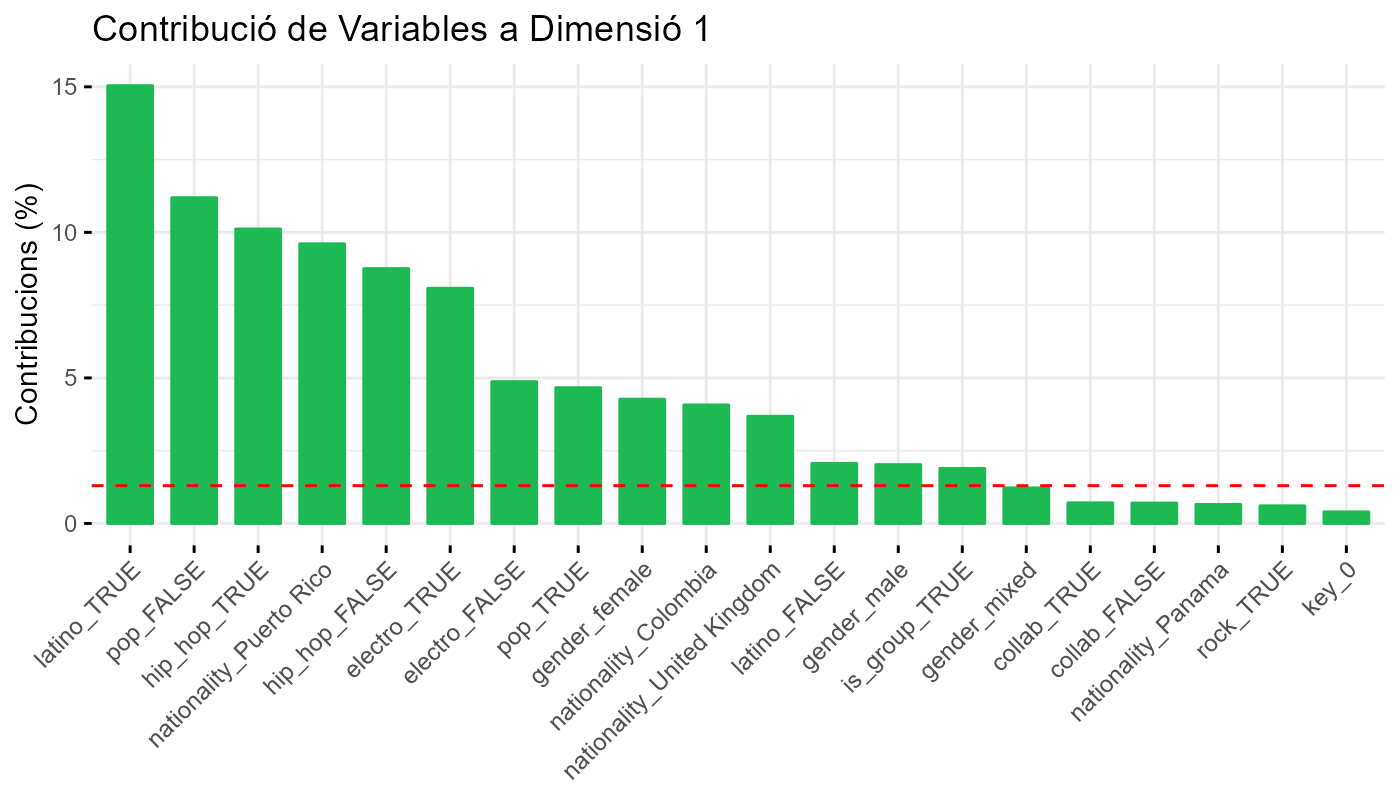
\includegraphics[width=0.95\linewidth]{Images/6_Factorial_Methods/ACM/ACM1_contribVars1.png}
    \caption{Contribució de les top 20 modalitats al primer eix}
    \label{fig:ACM1_contribVars1}
    \end{minipage}%
    \begin{minipage}{.5\textwidth}
        \centering
        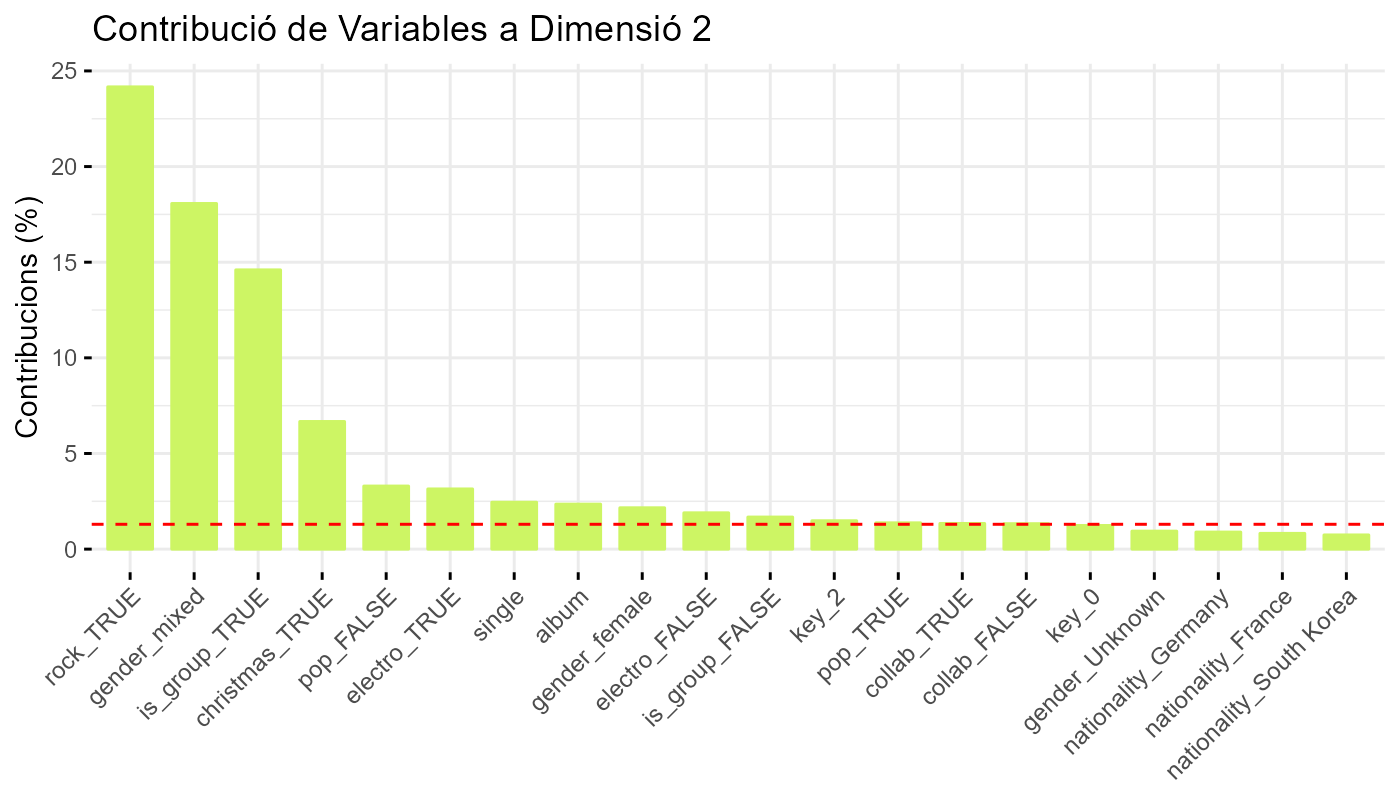
\includegraphics[width=0.95\linewidth]{Images/6_Factorial_Methods/ACM/ACM1_contribVars2.png}
    \caption{Contribució de les top 20 modalitats al segon eix}
    \label{fig:ACM1_contribVars2}
    \end{minipage}%
\end{figure}

Si observem la figura \ref{fig:ACM1_variablesCos2} i ens fixem només en les modalitats de colors no verds (aquelles que aportin més \textit{cos2}), veiem com el primer eix marca una divisió entre cançons \textit{pop} i \textit{electro} en la seva part positiva, i \textit{hip\_hop} i \textit{latino} en la part negativa de l'eix. A més, trobem les nacionalitats de Colòmbia i Puerto Rico completament relacionades amb el gènere \textit{latino} (part esquerra de l'eix), mentre que la nacionalitat de UK Unit es troba cap a la dreta, més relacionada amb \textit{pop} i \textit{electro}. També es pot veure com el gènere d'artistes femenines es troba a la dreta d'aquest primer eix, mentre que el masculí queda en la part negativa.

Per una altra banda, al segon eix (figura \ref{fig:ACM1_variablesCos2}) trobem clarament destacats els gèneres \textit{rock} i \textit{christmas} en la part positiva. \textit{is\_group\_TRUE} (encarregada d'indicar aquelles cançons compostes per grups) també es troba en la part superior de l'eix, segurament estant correlacionada amb els gèneres ja anomenats. Finalment, cal destacar que la part negativa de l'eix està bastant poc marcada, sense tenir cap modalitat amb un fort valor de \textit{cos2} que ens faciliti la seva classificació. Així i tot, cal destacar també la petita però remarcable relació d'aquest eix amb àlbums i singles, trobant-se els primers en la part positiva de l'eix, i els segons en la negativa.

\begin{figure}[H]
    \centering
    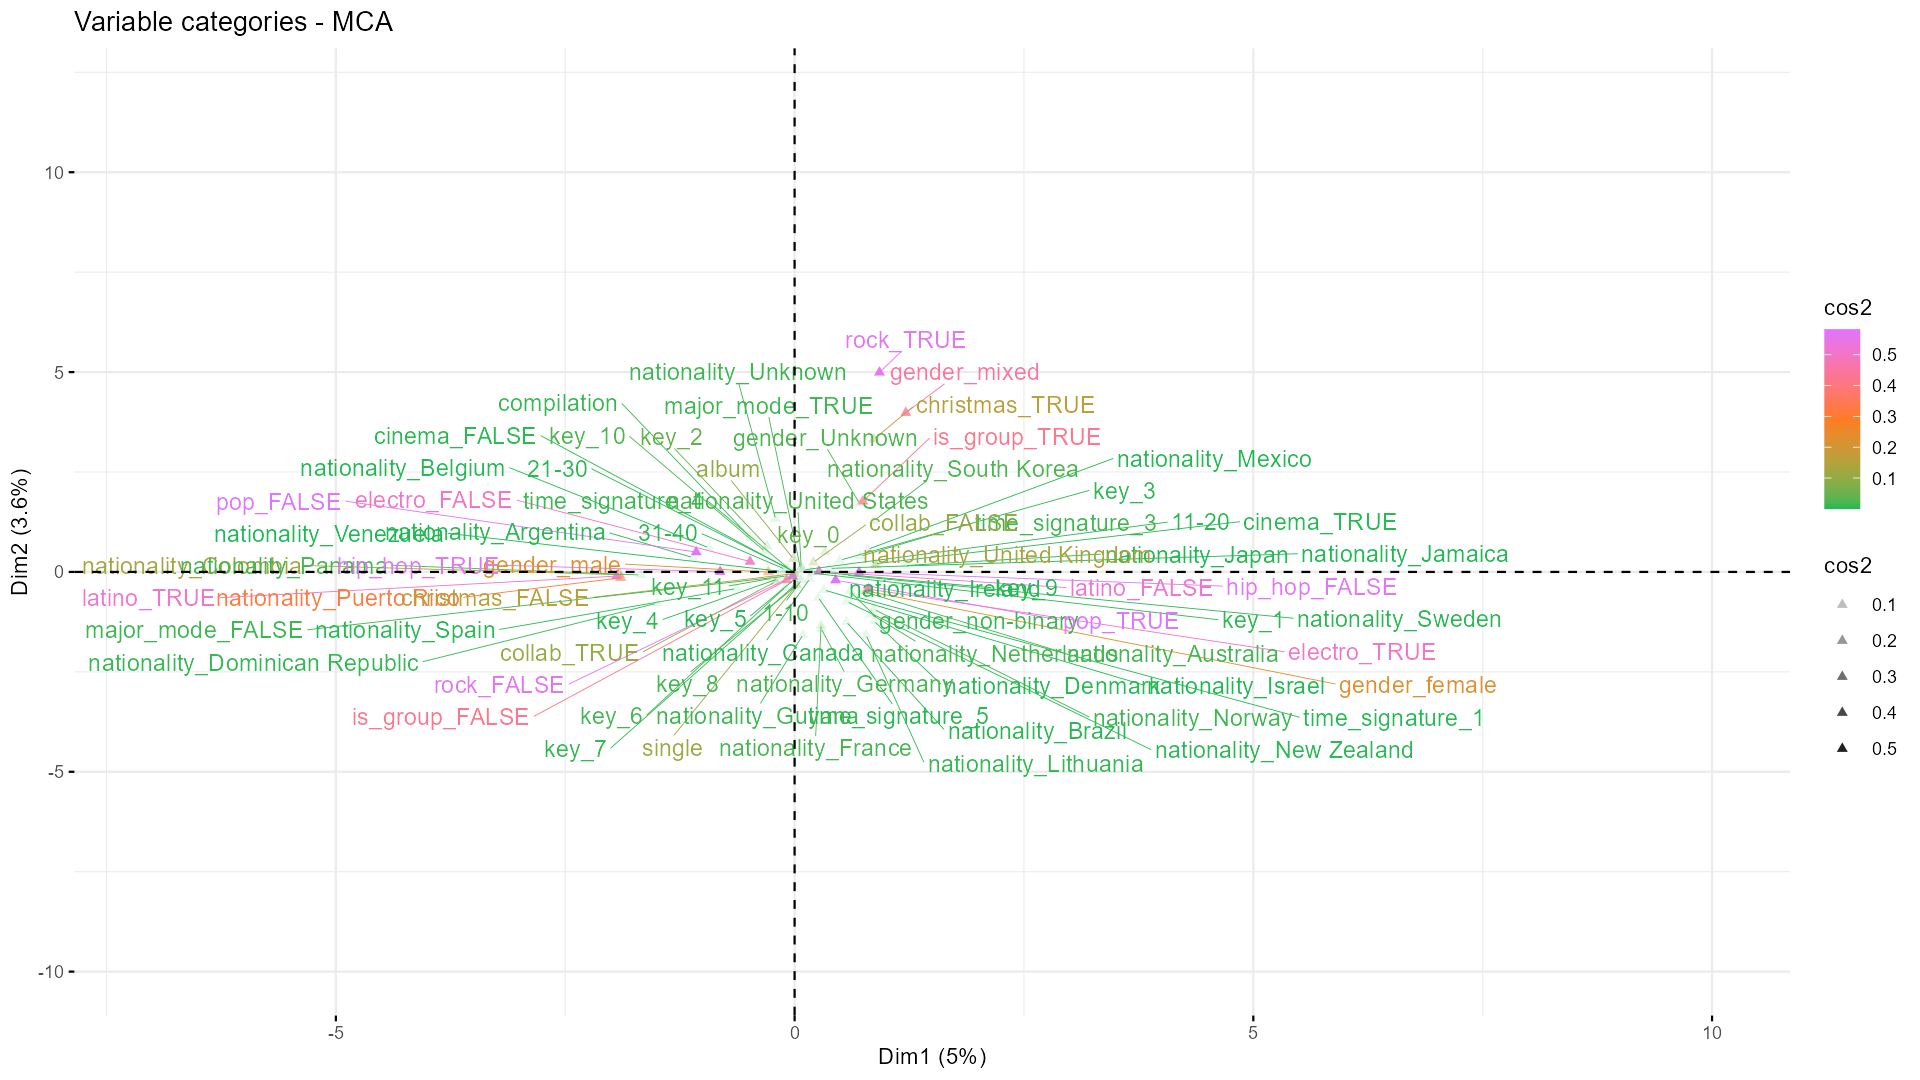
\includegraphics[width=0.8\linewidth]{Images/6_Factorial_Methods/ACM/ACM1_variablesCos2.png}
    \caption{Projecció de les modalitats utilitzades pel \textit{ACM}, acolorides segons el seu nivell de \textit{cos2}}
    \label{fig:ACM1_variablesCos2}
\end{figure}

Finalment, amb l'objectiu d'interpretar encara millor la projecció de les dades en aquests primers dos eixos, s'han creat les següents figures, que comparen la projecció de les cançons en funció d'algunes variables categòriques. En la figura \ref{fig:ACM1_indByGender}, s'observa clarament com el gènere masculí es troba cap a l'esquerra, al costat contrari que el femení. També es pot veure com el gènere \textit{mixed} (que fa referència a grups o bandes), es troba en la part positiva del primer eix, cosa completament relacionat amb la figura \ref{fig:ACM1_indByIsGroup}, on veiem com els grups també es troben en la part superior del gràfic, a diferència dels artistes que no formen part de grups. Per una altra banda, els singles també semblen trobar-se en la part superior del gràfic, tot i que sembla que es trobin sempre sobre els cúmuls de punts, dividint aquests cúmuls entre singles i àlbums (veure figura \ref{fig:ACM1_indByVarsAlbum}).


\begin{figure}[H]
    \centering
    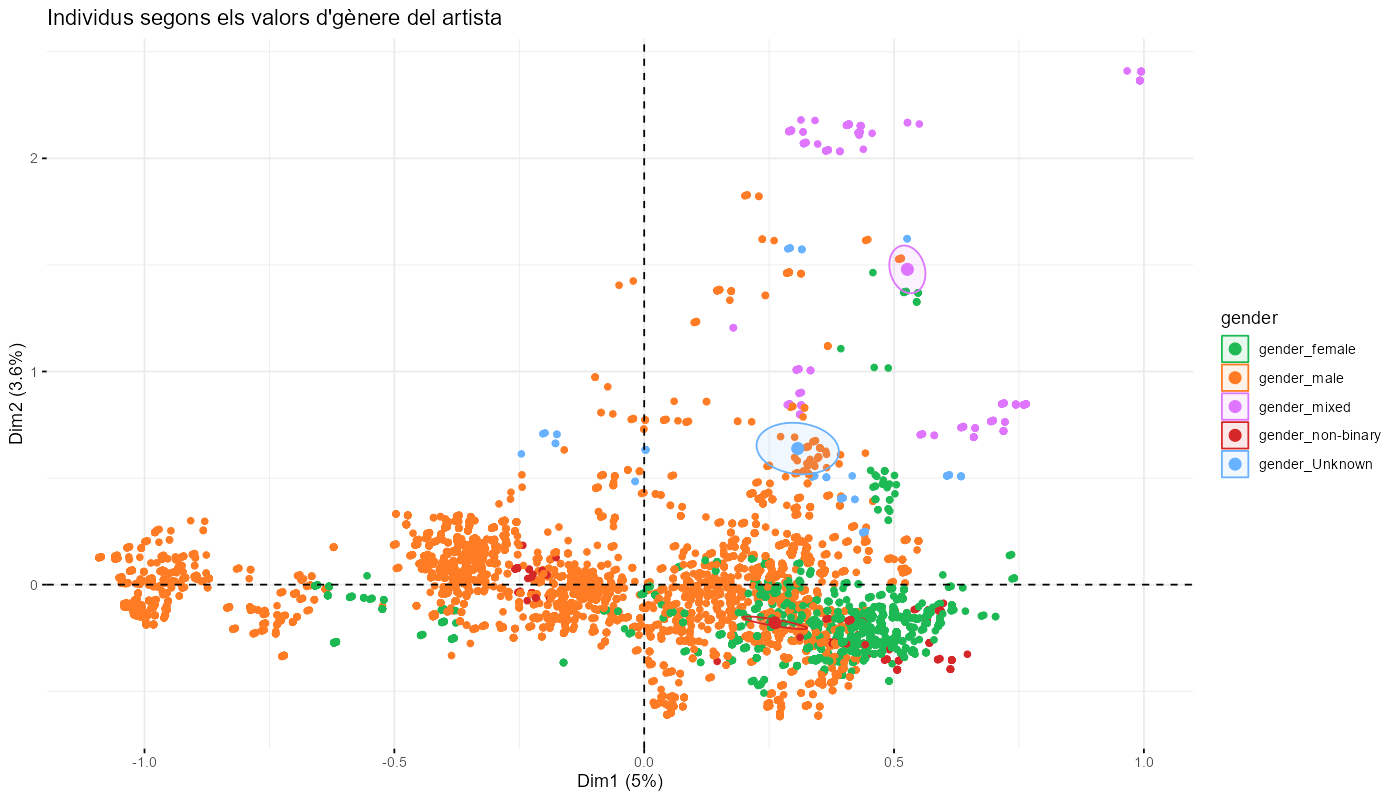
\includegraphics[width=0.7\linewidth]{Images/6_Factorial_Methods/ACM/ACM1_indByGender.png}
    \caption{Projecció dels individus del \textit{ACM} segons la variable \textit{gender}}
    \label{fig:ACM1_indByGender}
\end{figure}

\begin{figure}[H]
    \centering
    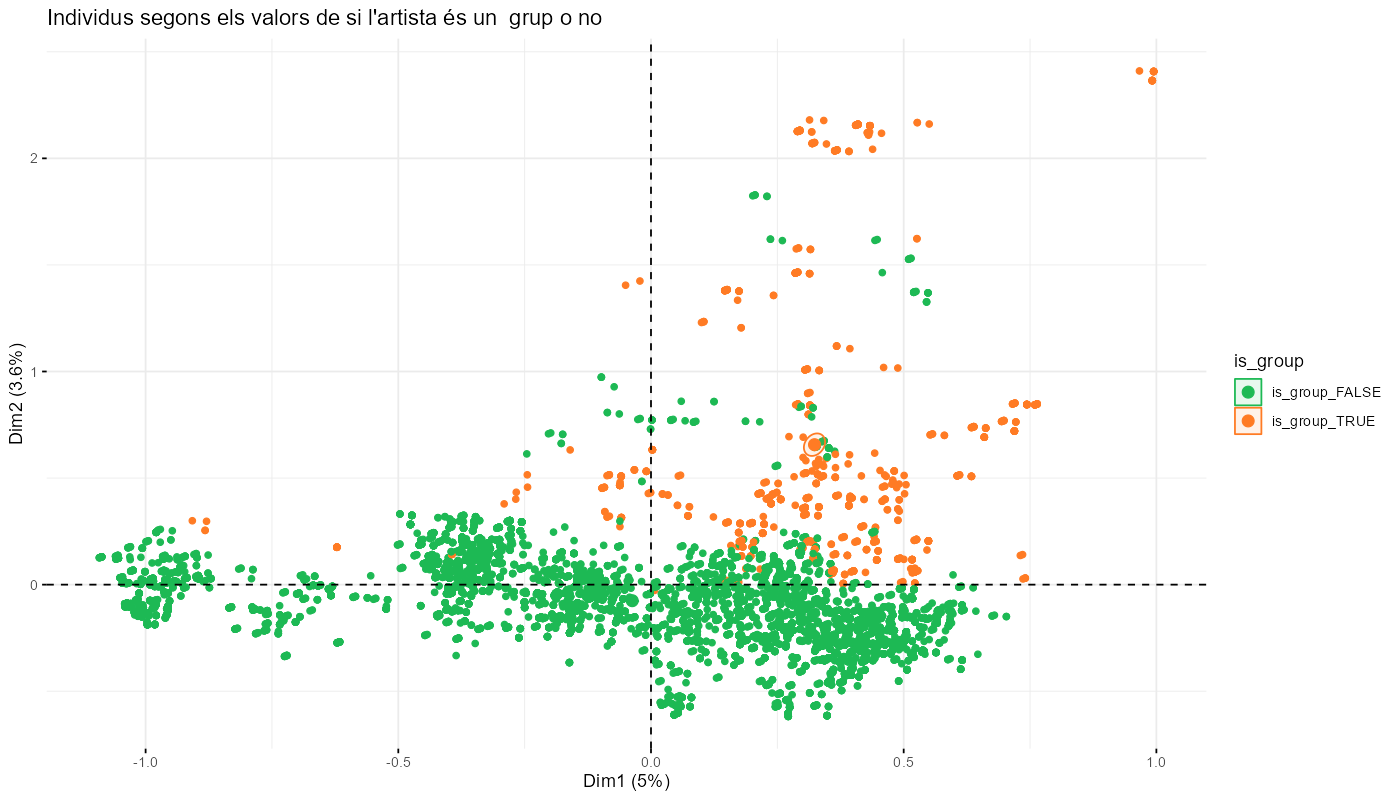
\includegraphics[width=0.7\linewidth]{Images/6_Factorial_Methods/ACM/ACM1_indByIsGroup.png}
    \caption{Projecció dels individus del \textit{ACM} segons la variable \textit{IsGroup}}
    \label{fig:ACM1_indByIsGroup}
\end{figure}

\begin{figure}[H]
    \centering
    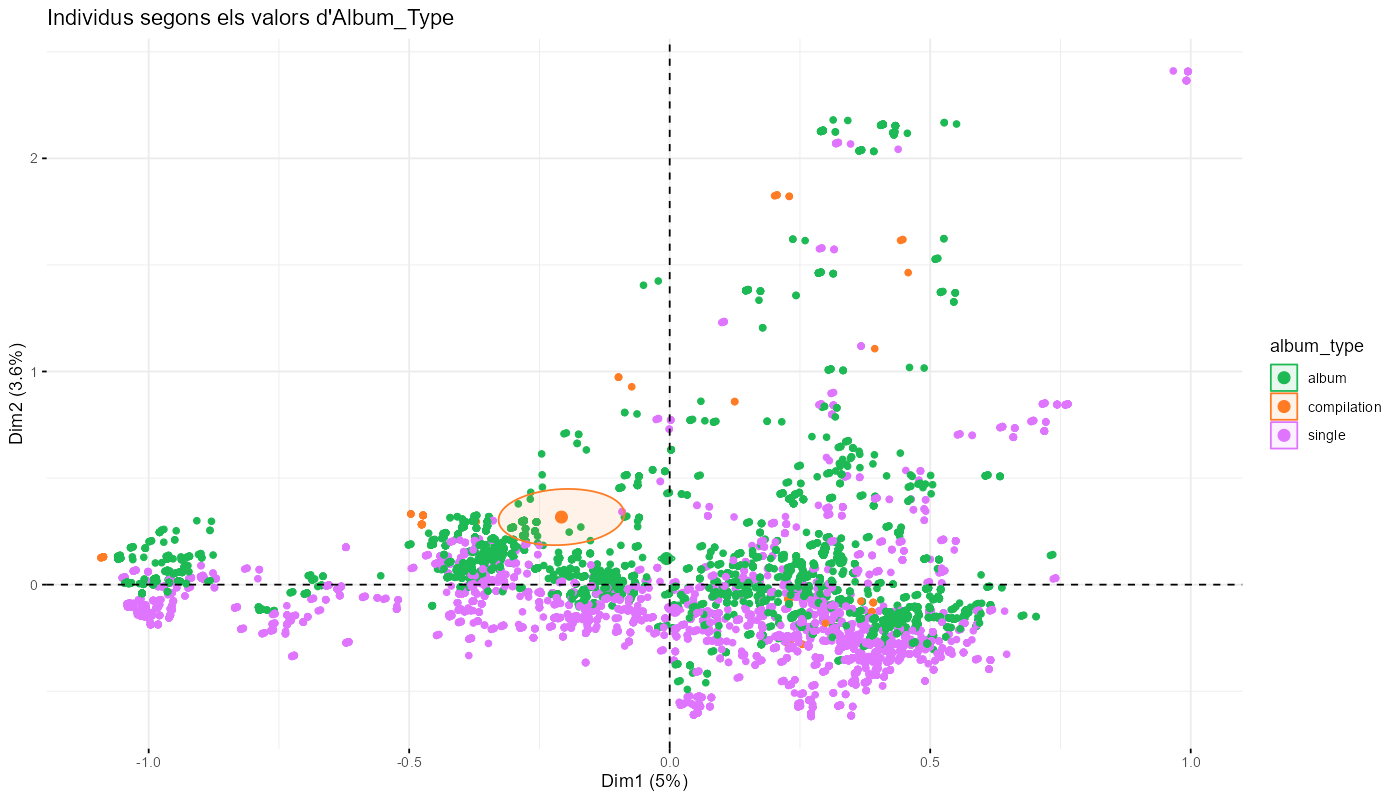
\includegraphics[width=0.7\linewidth]{Images/6_Factorial_Methods/ACM/ACM1_indByVarsAlbum.png}
    \caption{Projecció dels individus del \textit{ACM} segons la variable \textit{Album}}
    \label{fig:ACM1_indByVarsAlbum}
\end{figure}

En el que als gèneres musicals respecta, \textit{christmas} es concentra en la part superior de la gràfica (figura \ref{fig:ACM1_indByVarsChristmas}), estant relacionada clarament amb rock (figura \ref{fig:ACM1_indByVarsRock}). Les variables \textit{hip\_hop} i \textit{pop}, com era d'esperar, s'enfronten en el primer eix, quedant \textit{pop} a la dreta i \textit{hip\_hop} a l'esquerra de l'eix. La relació entre \textit{Electro} i \textit{hip\_hop} no és tan marcada com la de \textit{pop}, però si és cert que té una relació inversa amb \textit{hip\_hop} (figura \ref{fig:ACM1_indByElectro}). Finalment, cal destacar com les cançons que pertanyen al gènere \textit{latino} es troben completament aïllades cap a l'esquerra del gràfic, com es pot observar a la figura \ref{fig:ACM1_indByVarsLatino}.

\begin{figure}[H]
    \centering
    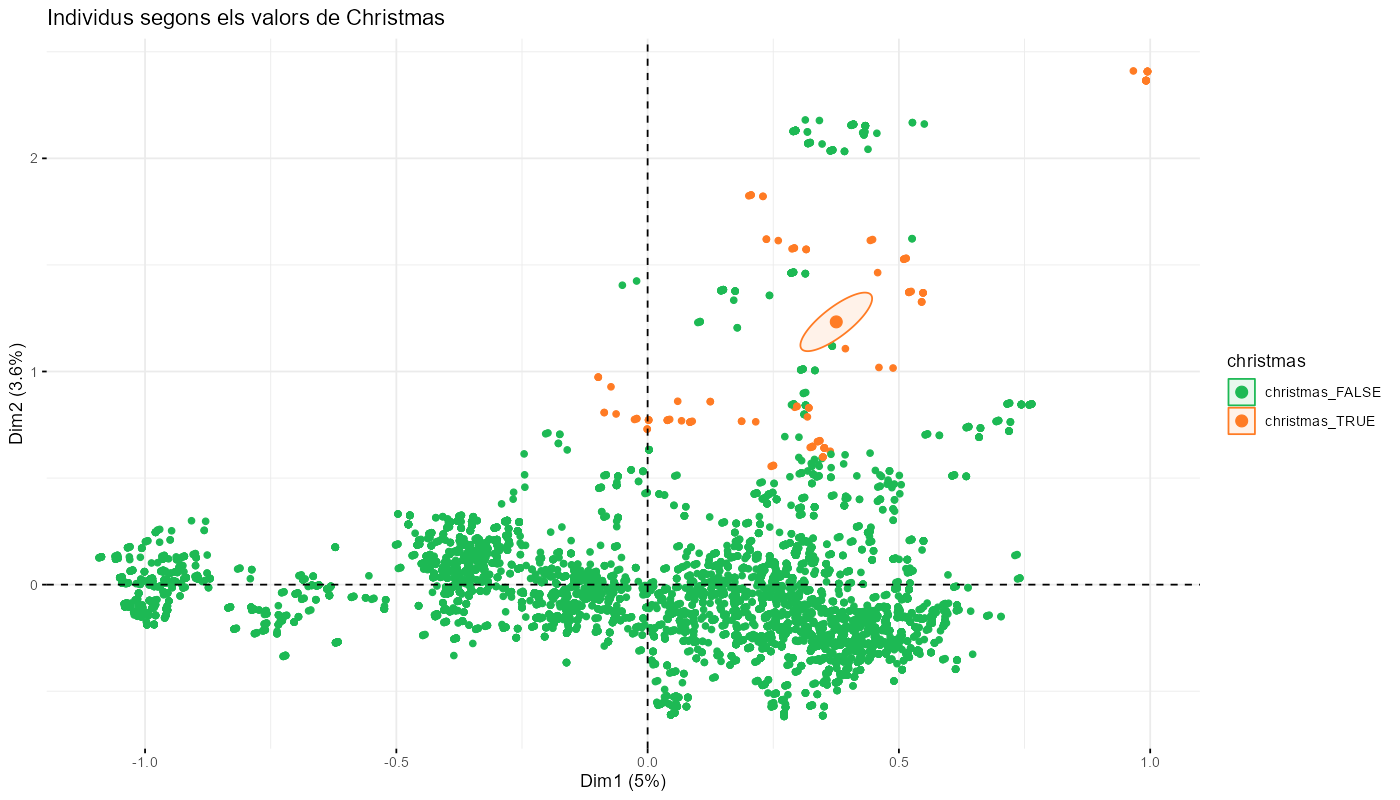
\includegraphics[width=0.7\linewidth]{Images/6_Factorial_Methods/ACM/ACM1_indByVarsChristmas.png}
    \caption{Projecció dels individus del \textit{ACM} segons la variable \textit{christmas}}
    \label{fig:ACM1_indByVarsChristmas}
\end{figure}

\begin{figure}[H]
    \centering
    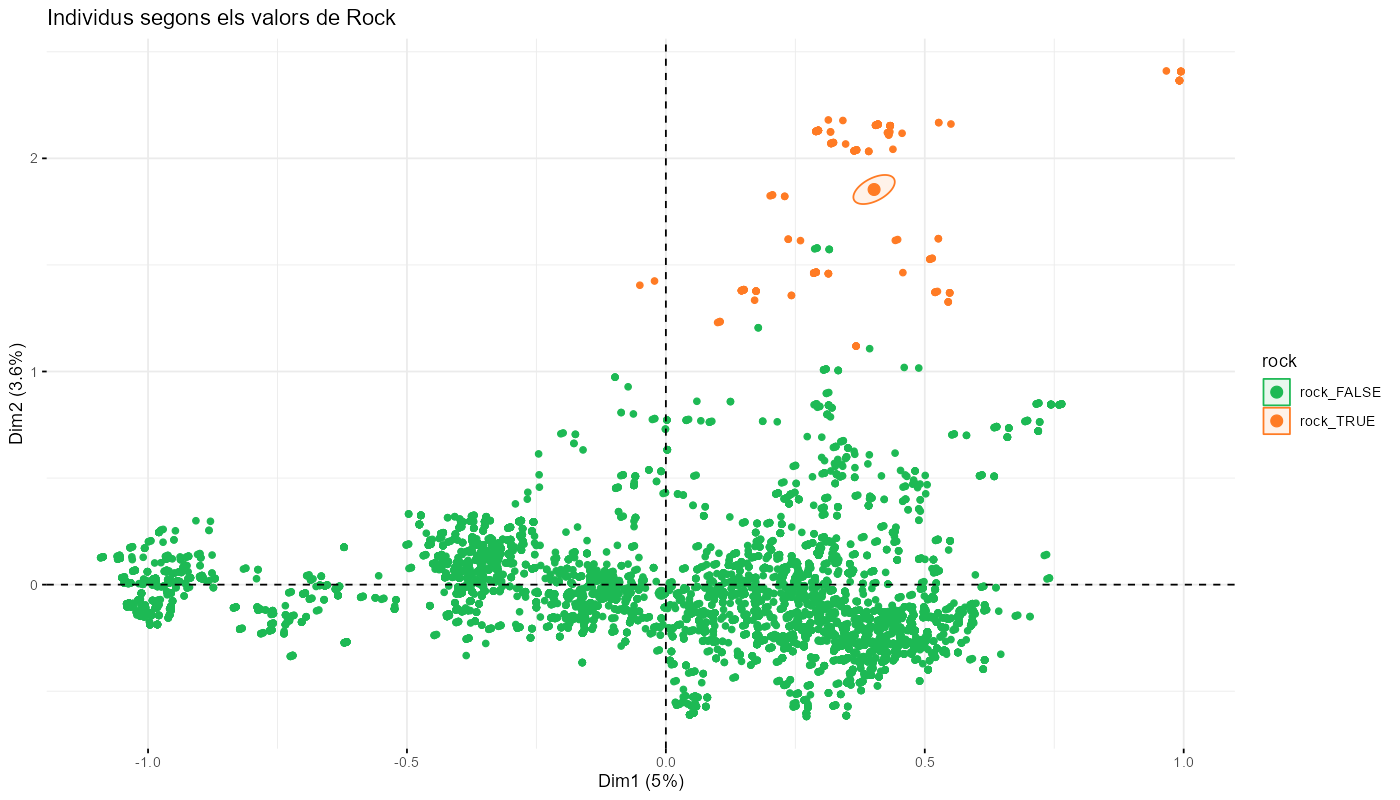
\includegraphics[width=0.7\linewidth]{Images/6_Factorial_Methods/ACM/ACM1_indByVarsRock.png}
    \caption{Projecció dels individus del \textit{ACM} segons la variable \textit{rock}}
    \label{fig:ACM1_indByVarsRock}
\end{figure}

\begin{figure}[H]
    \centering
    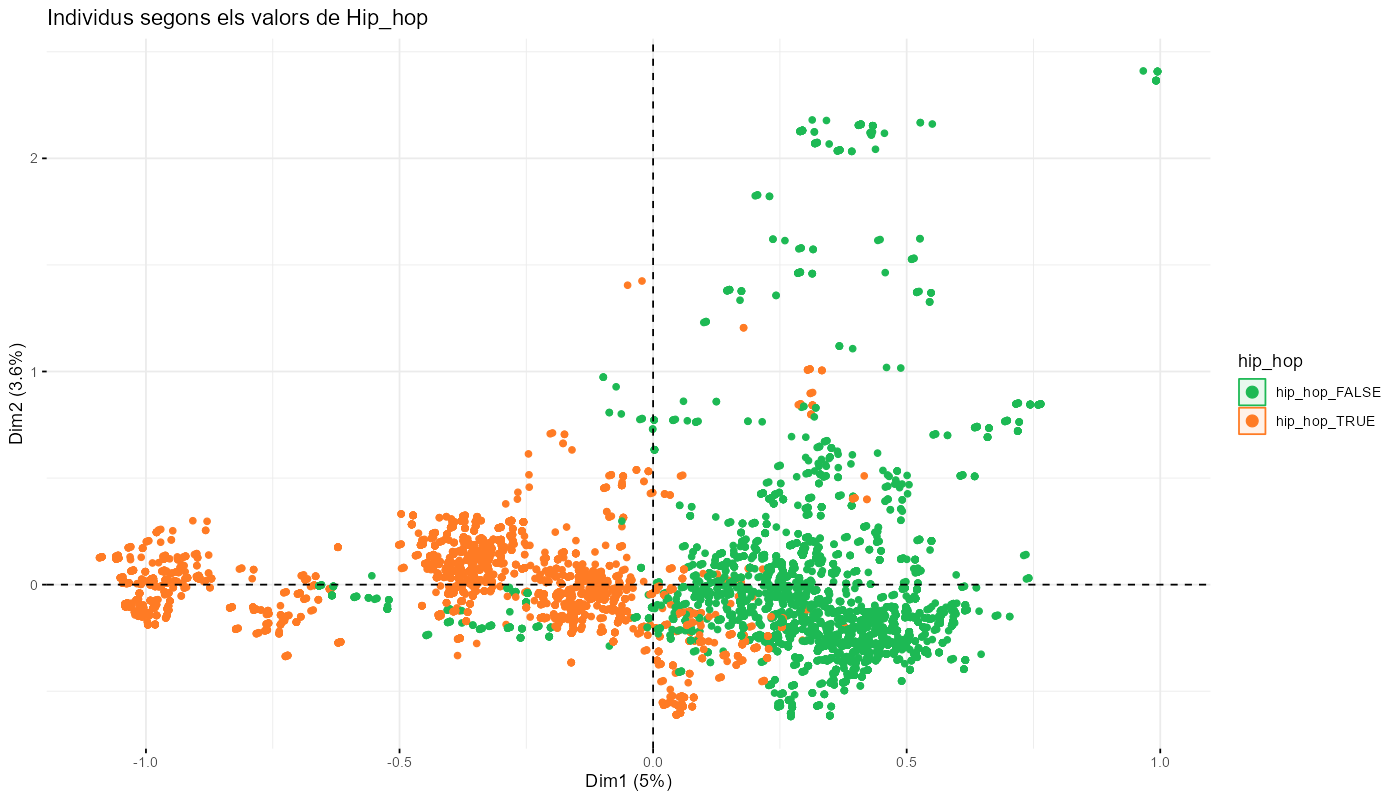
\includegraphics[width=0.7\linewidth]{Images/6_Factorial_Methods/ACM/ACM1_indByVarsHipHop.png}
    \caption{Projecció dels individus del \textit{ACM} segons la variable \textit{hip\_hop}}
    \label{fig:ACM1_indByVarsHipHop}
\end{figure}

\begin{figure}[H]
    \centering
    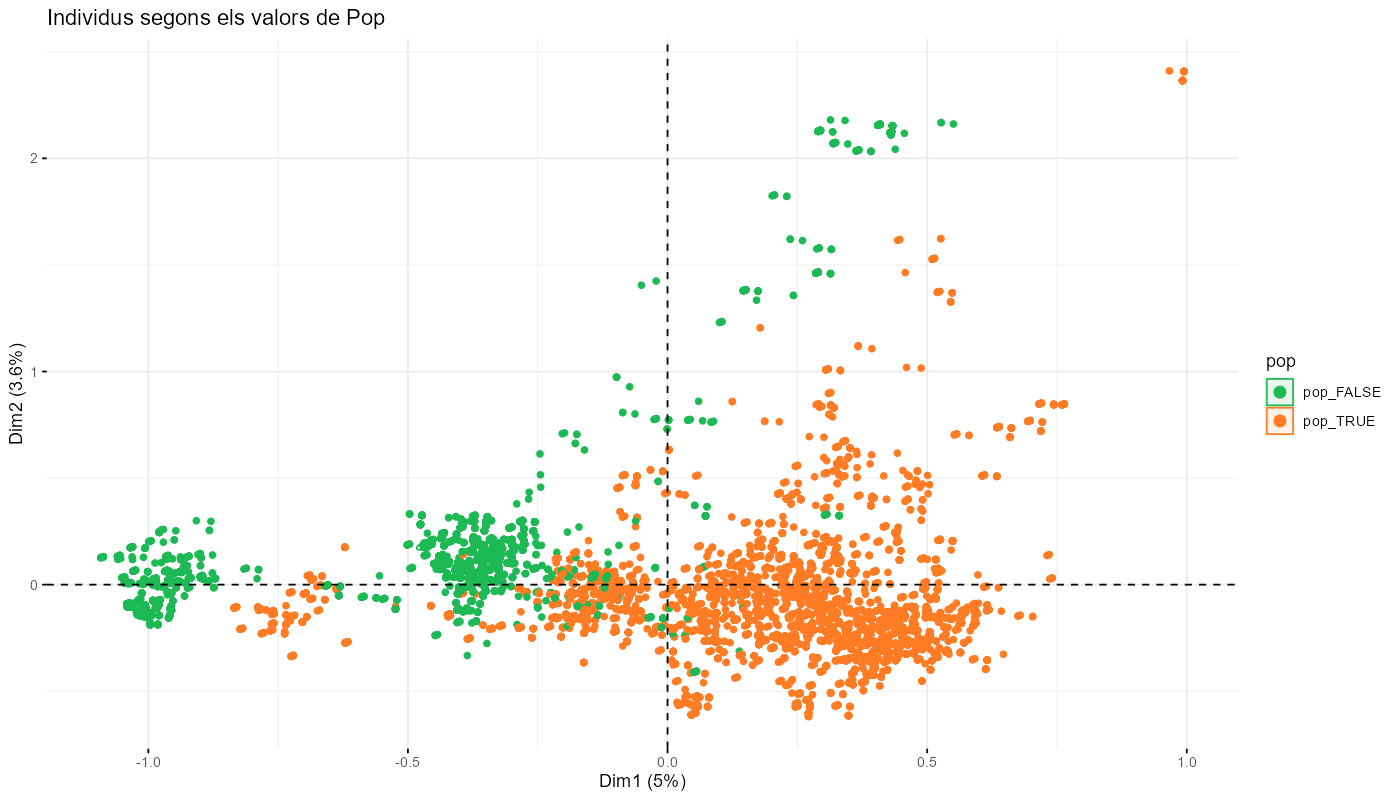
\includegraphics[width=0.7\linewidth]{Images/6_Factorial_Methods/ACM/ACM1_indByVarsPop.png}
    \caption{Projecció dels individus del \textit{ACM} segons la variable \textit{pop}}
    \label{fig:ACM1_indByVarsPop}
\end{figure}

\begin{figure}[H]
    \centering
    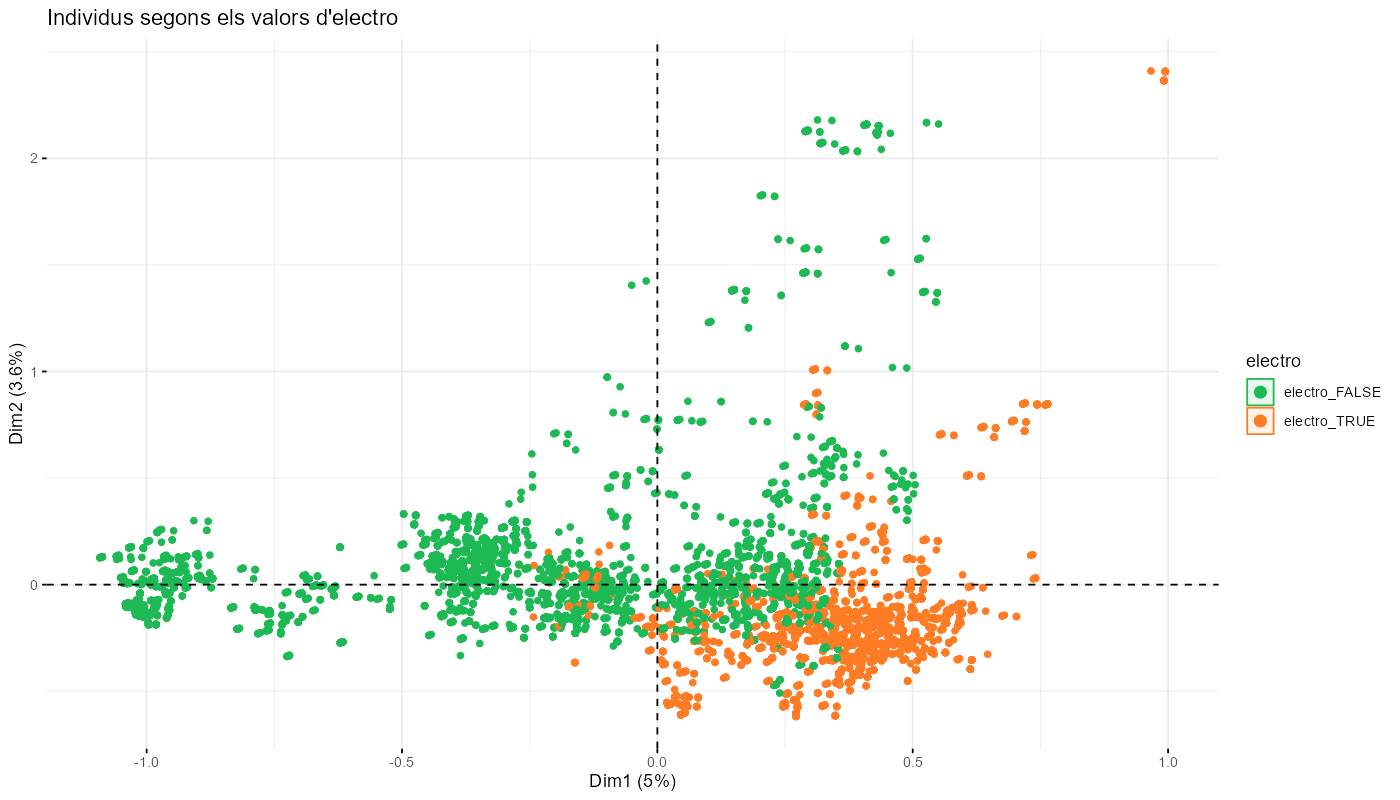
\includegraphics[width=0.7\linewidth]{Images/6_Factorial_Methods/ACM/ACM1_indByElectro.png}
    \caption{Projecció dels individus del \textit{ACM} segons la variable \textit{electro}}
    \label{fig:ACM1_indByElectro}
\end{figure}

\begin{figure}[H]
    \centering
    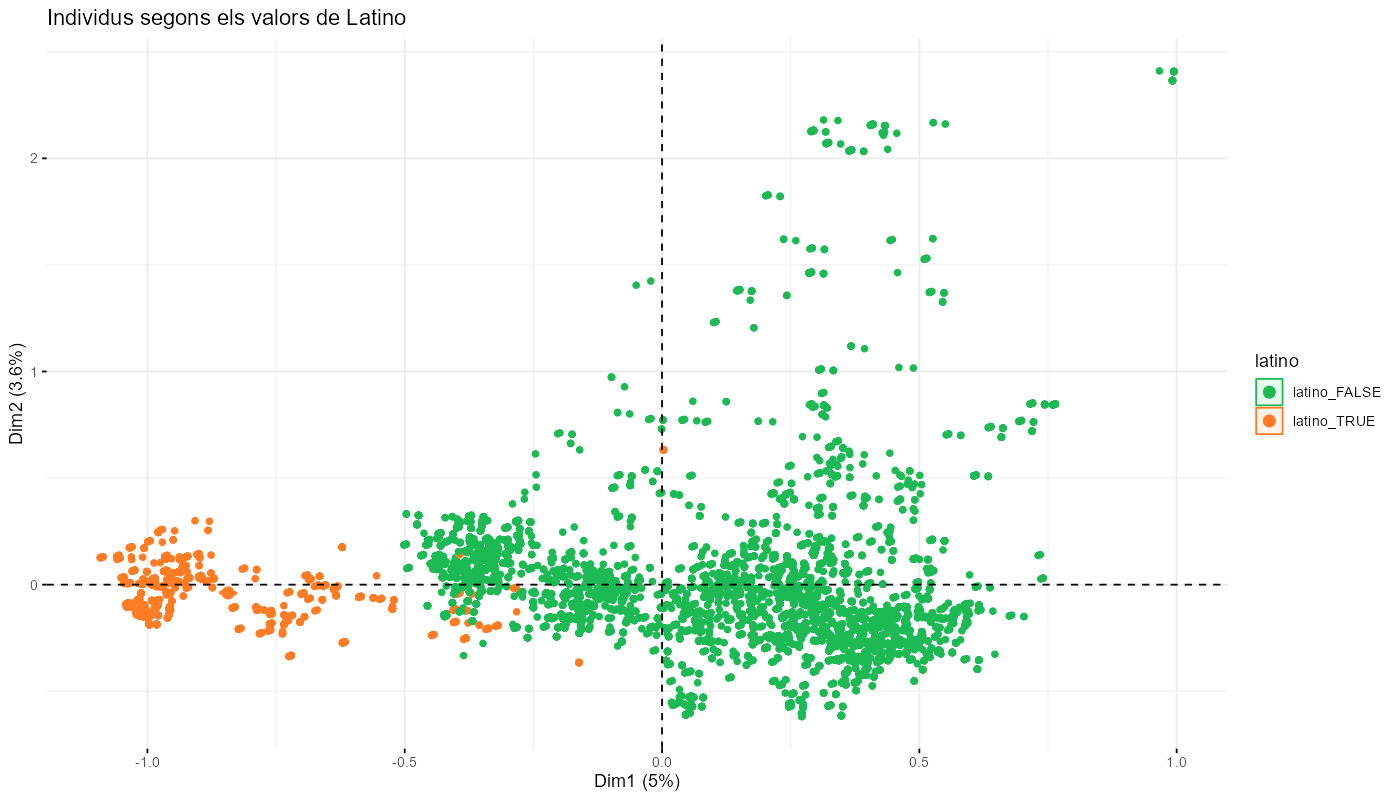
\includegraphics[width=0.7\linewidth]{Images/6_Factorial_Methods/ACM/ACM1_indByVarsLatino.png}
    \caption{Projecció dels individus del \textit{ACM} segons la variable \textit{latino}}
    \label{fig:ACM1_indByVarsLatino}
\end{figure}

\subsubsection{Interpretació final dels eixos}

En conclusió, donades les interpretacions fetes a la secció prèvia, podem extraure els següents significats pels eixos del \textit{ACM} que s'utilitzarà per entrenar la xarxa neuronal:

\begin{itemize}
    \item Eix 1: \begin{itemize}
        \item \textbf{Part Positiva:} \textit{pop}, \textit{electro}, artistes femenines i nacionalitat de Gran Bretanya.
        \item \textbf{Part Negativa:}\textit{ hip\_hop}, \textit{latino}, artistes masculins i nacionalitats de Colòmbia i Puerto Rico.
    \end{itemize}
    \item Eix 2: \begin{itemize}
        \item \textbf{Part Positiva:} \textit{Christmas}, \textit{rock}, àlbums i bandes.
        \item \textbf{Part Negativa:} singles i artistes individuals.
    \end{itemize}
\end{itemize}

En general, cal destacar que tot i que aquests resultats semblin prou lògics, l'explicabilitat dels dos primers eixos encara és molt baixa (inferior al 10\%), així que les conclusions extradides no tindrien per què ser certes. Així i tot, cal remarcar que l'objectiu d'aquest \textit{ACM} no era trobar grans conclusions, sinó projectar les nostres variables en dimensions que maximitzin la variància explicada, amb l'objectiu d'entrenar la xarxa neuronal amb millor rendiment.   

\subsection{Anàlisi de Components Principals}
A més de l'Anàlisi de Correspondències Múltiples per les variables categòriques, també s'ha realitzat un Anàlisi de Components Principals per les variables numèriques que la base de dades. Això ha permès fer una reducció de dimensionalitat i eliminar la correlació entre les variables del dataset (ja que tots els components principals són ortogonals).

Per tal de realitzar aquest anàlisi, no s'han considerat totes les variables de la base de dades original, ja que n'hi ha que no aportaven gran informació o que eren molt similars. Per tant, tal i com es va fer la prèvia assignatura (Modelització Estadística),  no s'han considerat les variables album\_popularity i artist\_followers, ja que sempre tenen valors molt similars a la variable track\_popularity; és a dir, estan molt correlacionades i, si s'afegissin les 3, els primers components representarien principalment la correlació entre aquestes variables, però podria haver altres patrons o estructures en la base de dades que no es veurien representades en els components.

Per altra banda, no s'han considerat certes variables categòriques amb moltes classes a l'hora de projectar els seus centroides en els diferents components, ja que hi hauria masses centroides i no es podrien interpretar correctament els resultats. Algunes d'aquestes variables són track\_name, artist\_name, album\_label, lyrics, city, etc.

L'objectiu final és obtenir els primers \textit{N} components que representin el 80\% de la variància de les dades originals, per tal d'eliminar soroll i reduir bastant la dimensionalitat. Posteriorment, s'entrenarà un model amb aquestes dades (i amb les de l'ACM), però abans d'això s'interpretaran els diferents components per tal d'entendre què representa cada un d'ells.

Una vegada executat l'ACP, es pot veure en la figura \ref{fig:6_FM:variancia_per_components} es pot veure el percentatge de variància explicada per cada un dels components trobats. Es pot veure que el primer component no arriba ni tal sols al 20\% de la variància explicada, mentre que el segon component només n'explica aproximadament un 10\%. Això vol dir que en els gràfics bidimensionals que es facin hi haurà poca variància representada, de manera que no es poden prendre els resultats com a una representació totalment certa de la base de dades original.

\begin{figure}[H]
    \centering
    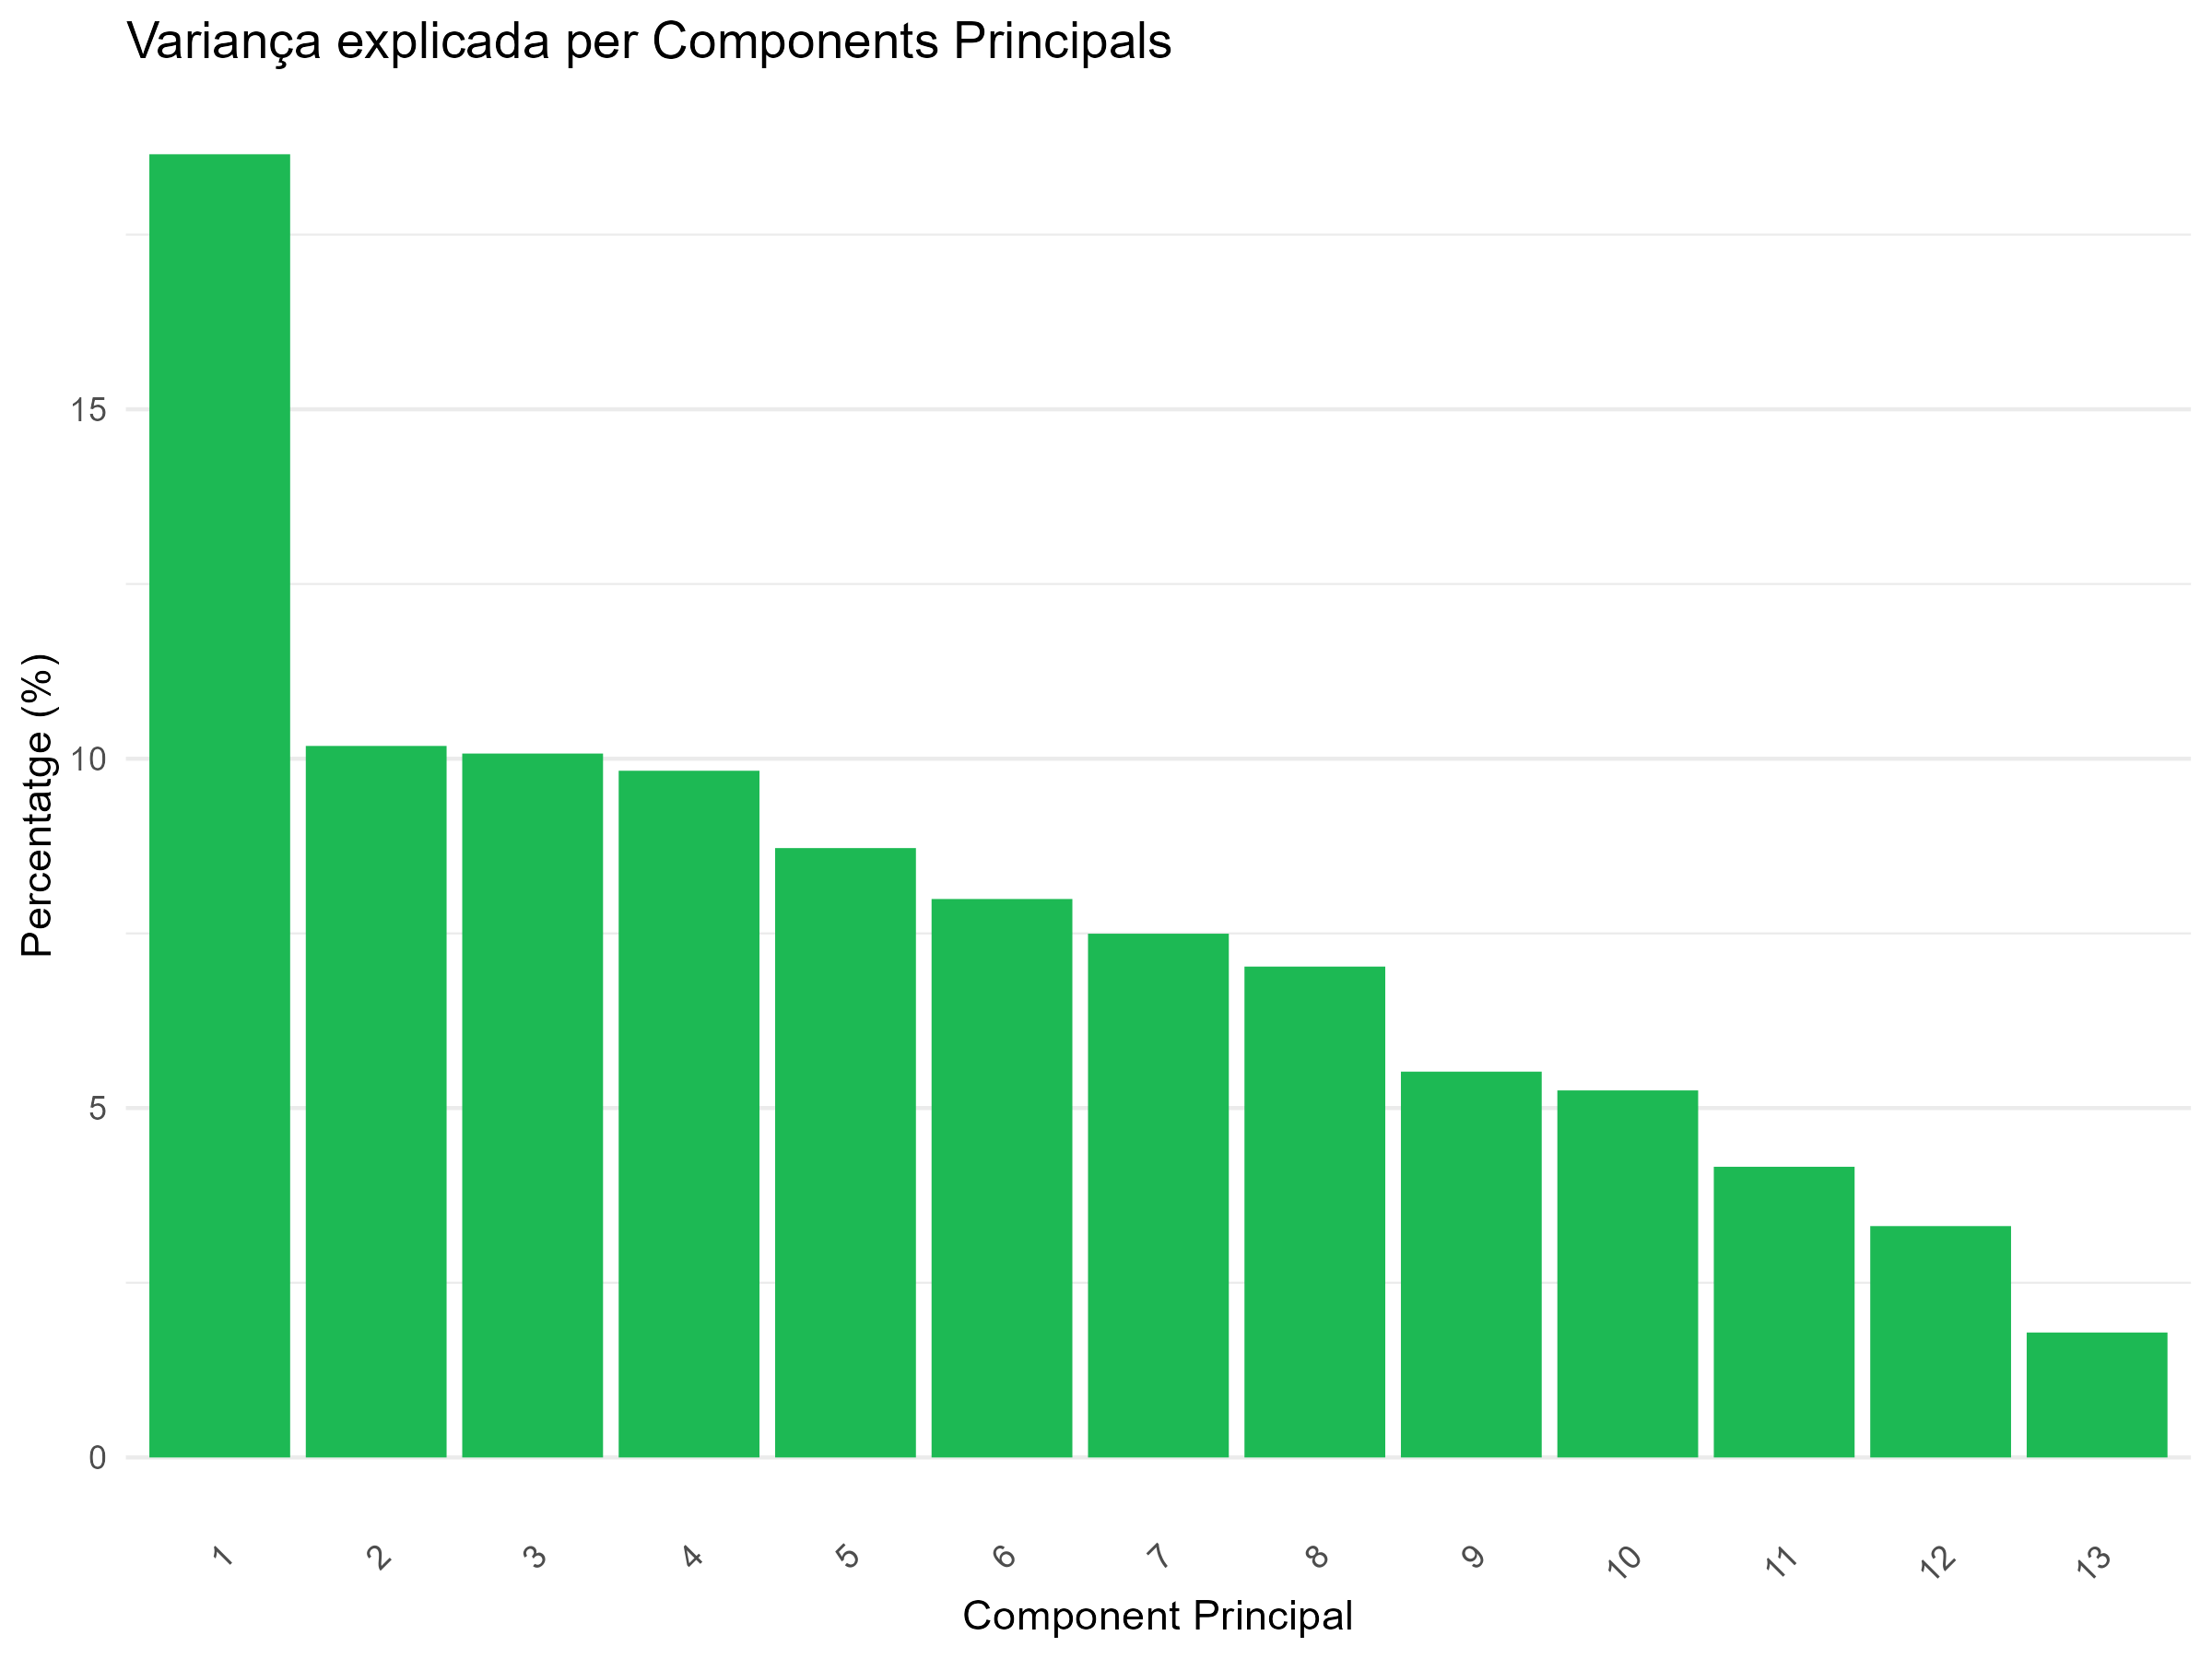
\includegraphics[width=0.8\linewidth]{Images/6_Factorial_Methods/ACP/Percentatge_varianca_per_component.png}
    \caption{Percentatge de variància explicada per cada un dels components principals}
    \label{fig:6_FM:variancia_per_components}
\end{figure}

Si es sumen aquests percentatges, es pot veure en la figura \ref{fig:6_FM:variancia_acumulada} que el nombre de components necessaris per representar un 80\% de la variància és \textit{N = 9}.

\begin{figure}[H]
    \centering
    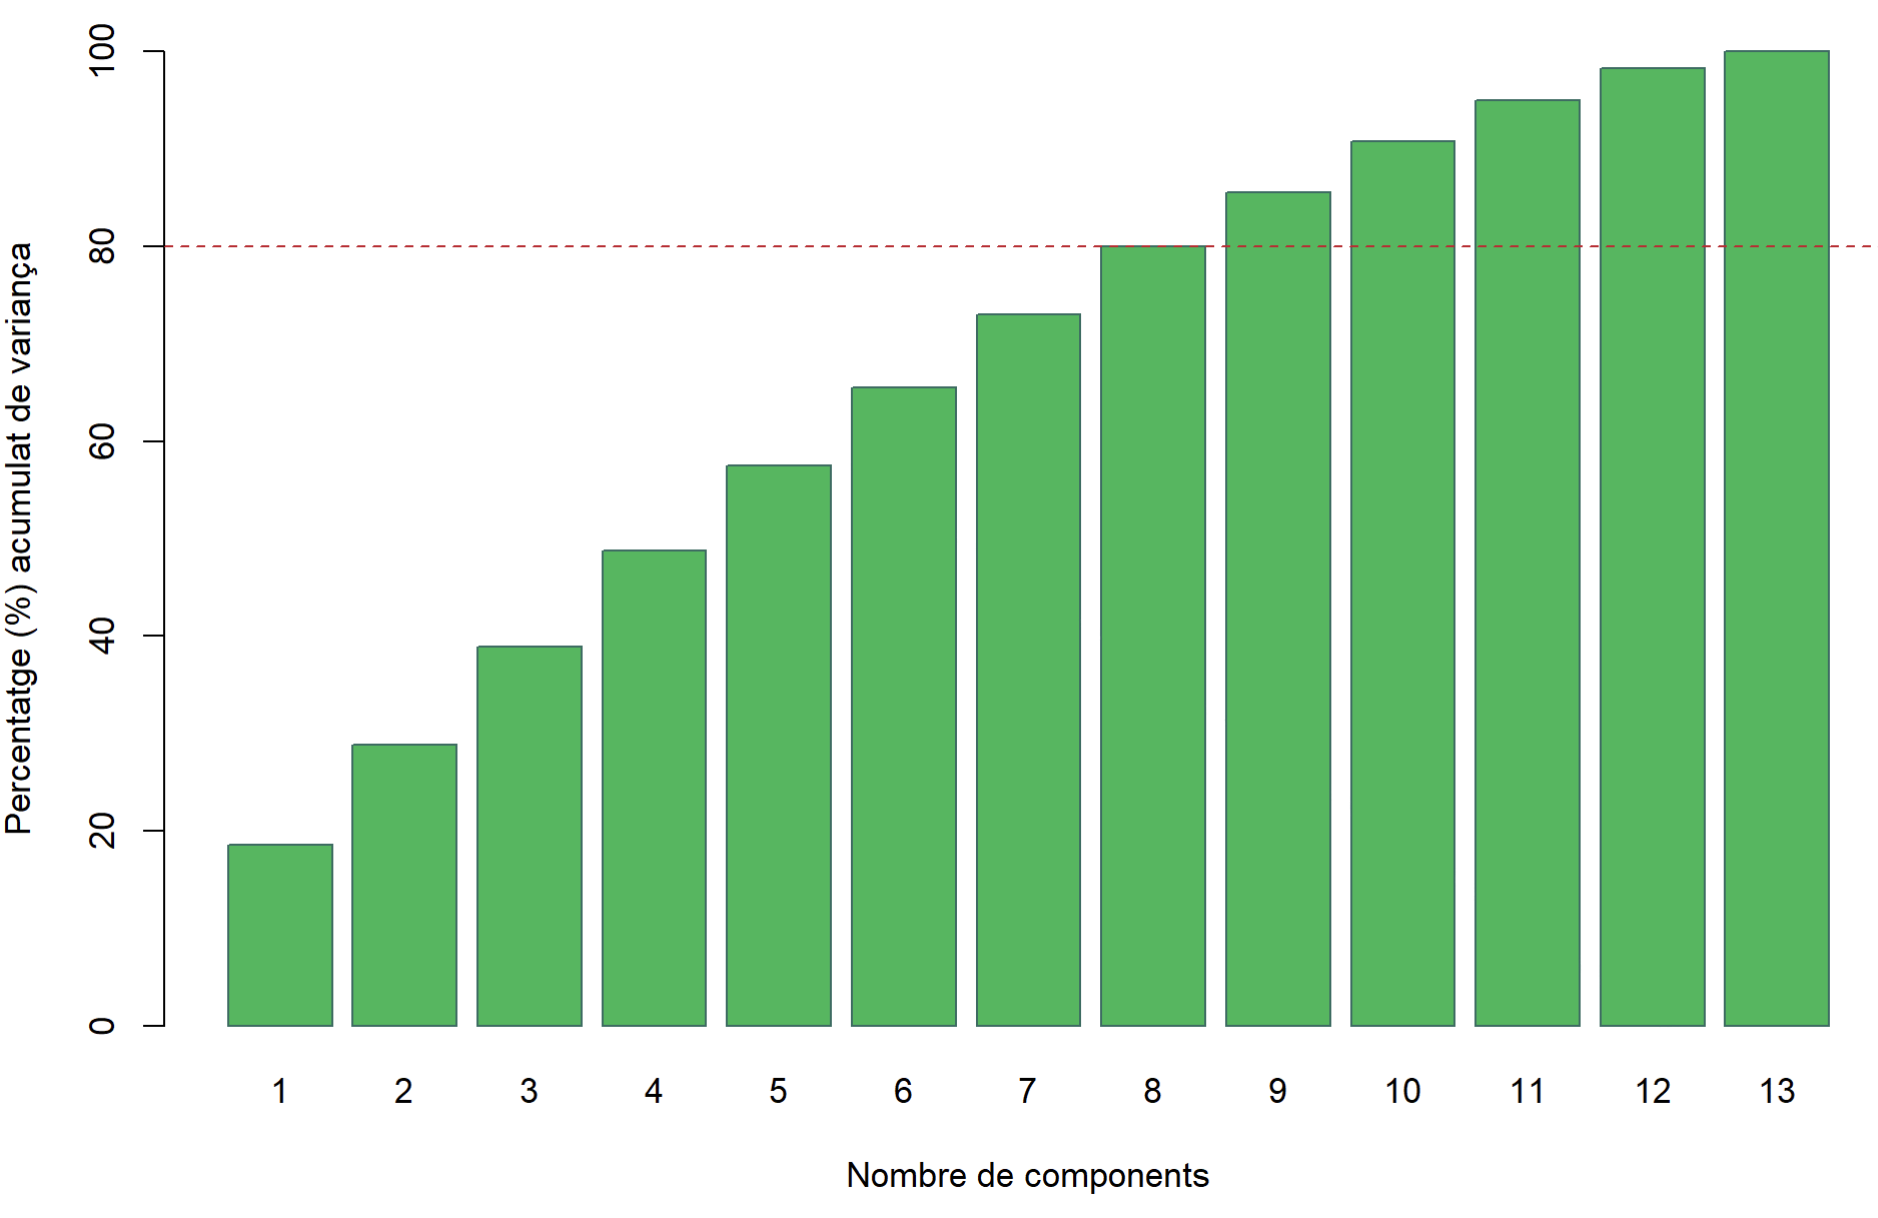
\includegraphics[width=0.8\linewidth]{Images/6_Factorial_Methods/ACP/Variancia_acumulada.png}
    \caption{Percentatge de variància acumulada en funció del nombre de components}
    \label{fig:6_FM:variancia_acumulada}
\end{figure}

\subsubsection{Variables numèriques i interpretació de components}

Seguidament, s'han projectat les variables numèriques a sobre dels diferents components per poder interpretar-los i etiquetar-los. S'ha de tenir en compte que molts d'aquests components expliquen un percentatge de variància molt baix de la base de dades, de manera que és difícil trobar interpretacions clares o representatives que permetin etiquetar-los.

En la figura \ref{fig:6_FM:ACP_C12} es poden veure els components 1 i 2, que junts representen pràcticament un 30\% de la variància. Es pot observar que el primer component està clarament marcat per una alta correlació negativa amb les variables energy, loudness i valence, mentre que té una alta correlació positiva amb la variable acousticness. Per tant, el primer component està relacionat amb la ``potència'' o ``energia'' de les cançons. Per altra banda, el segon component té principalment una alta correlació positiva amb tempo i artist\_popularity; i una correlació negativa amb valence, danceability i acousticness. Per tant, es podria dir que aquest component representa l'emoció de la cançó i el tipus d'artista.

\begin{figure}[H]
    \centering
    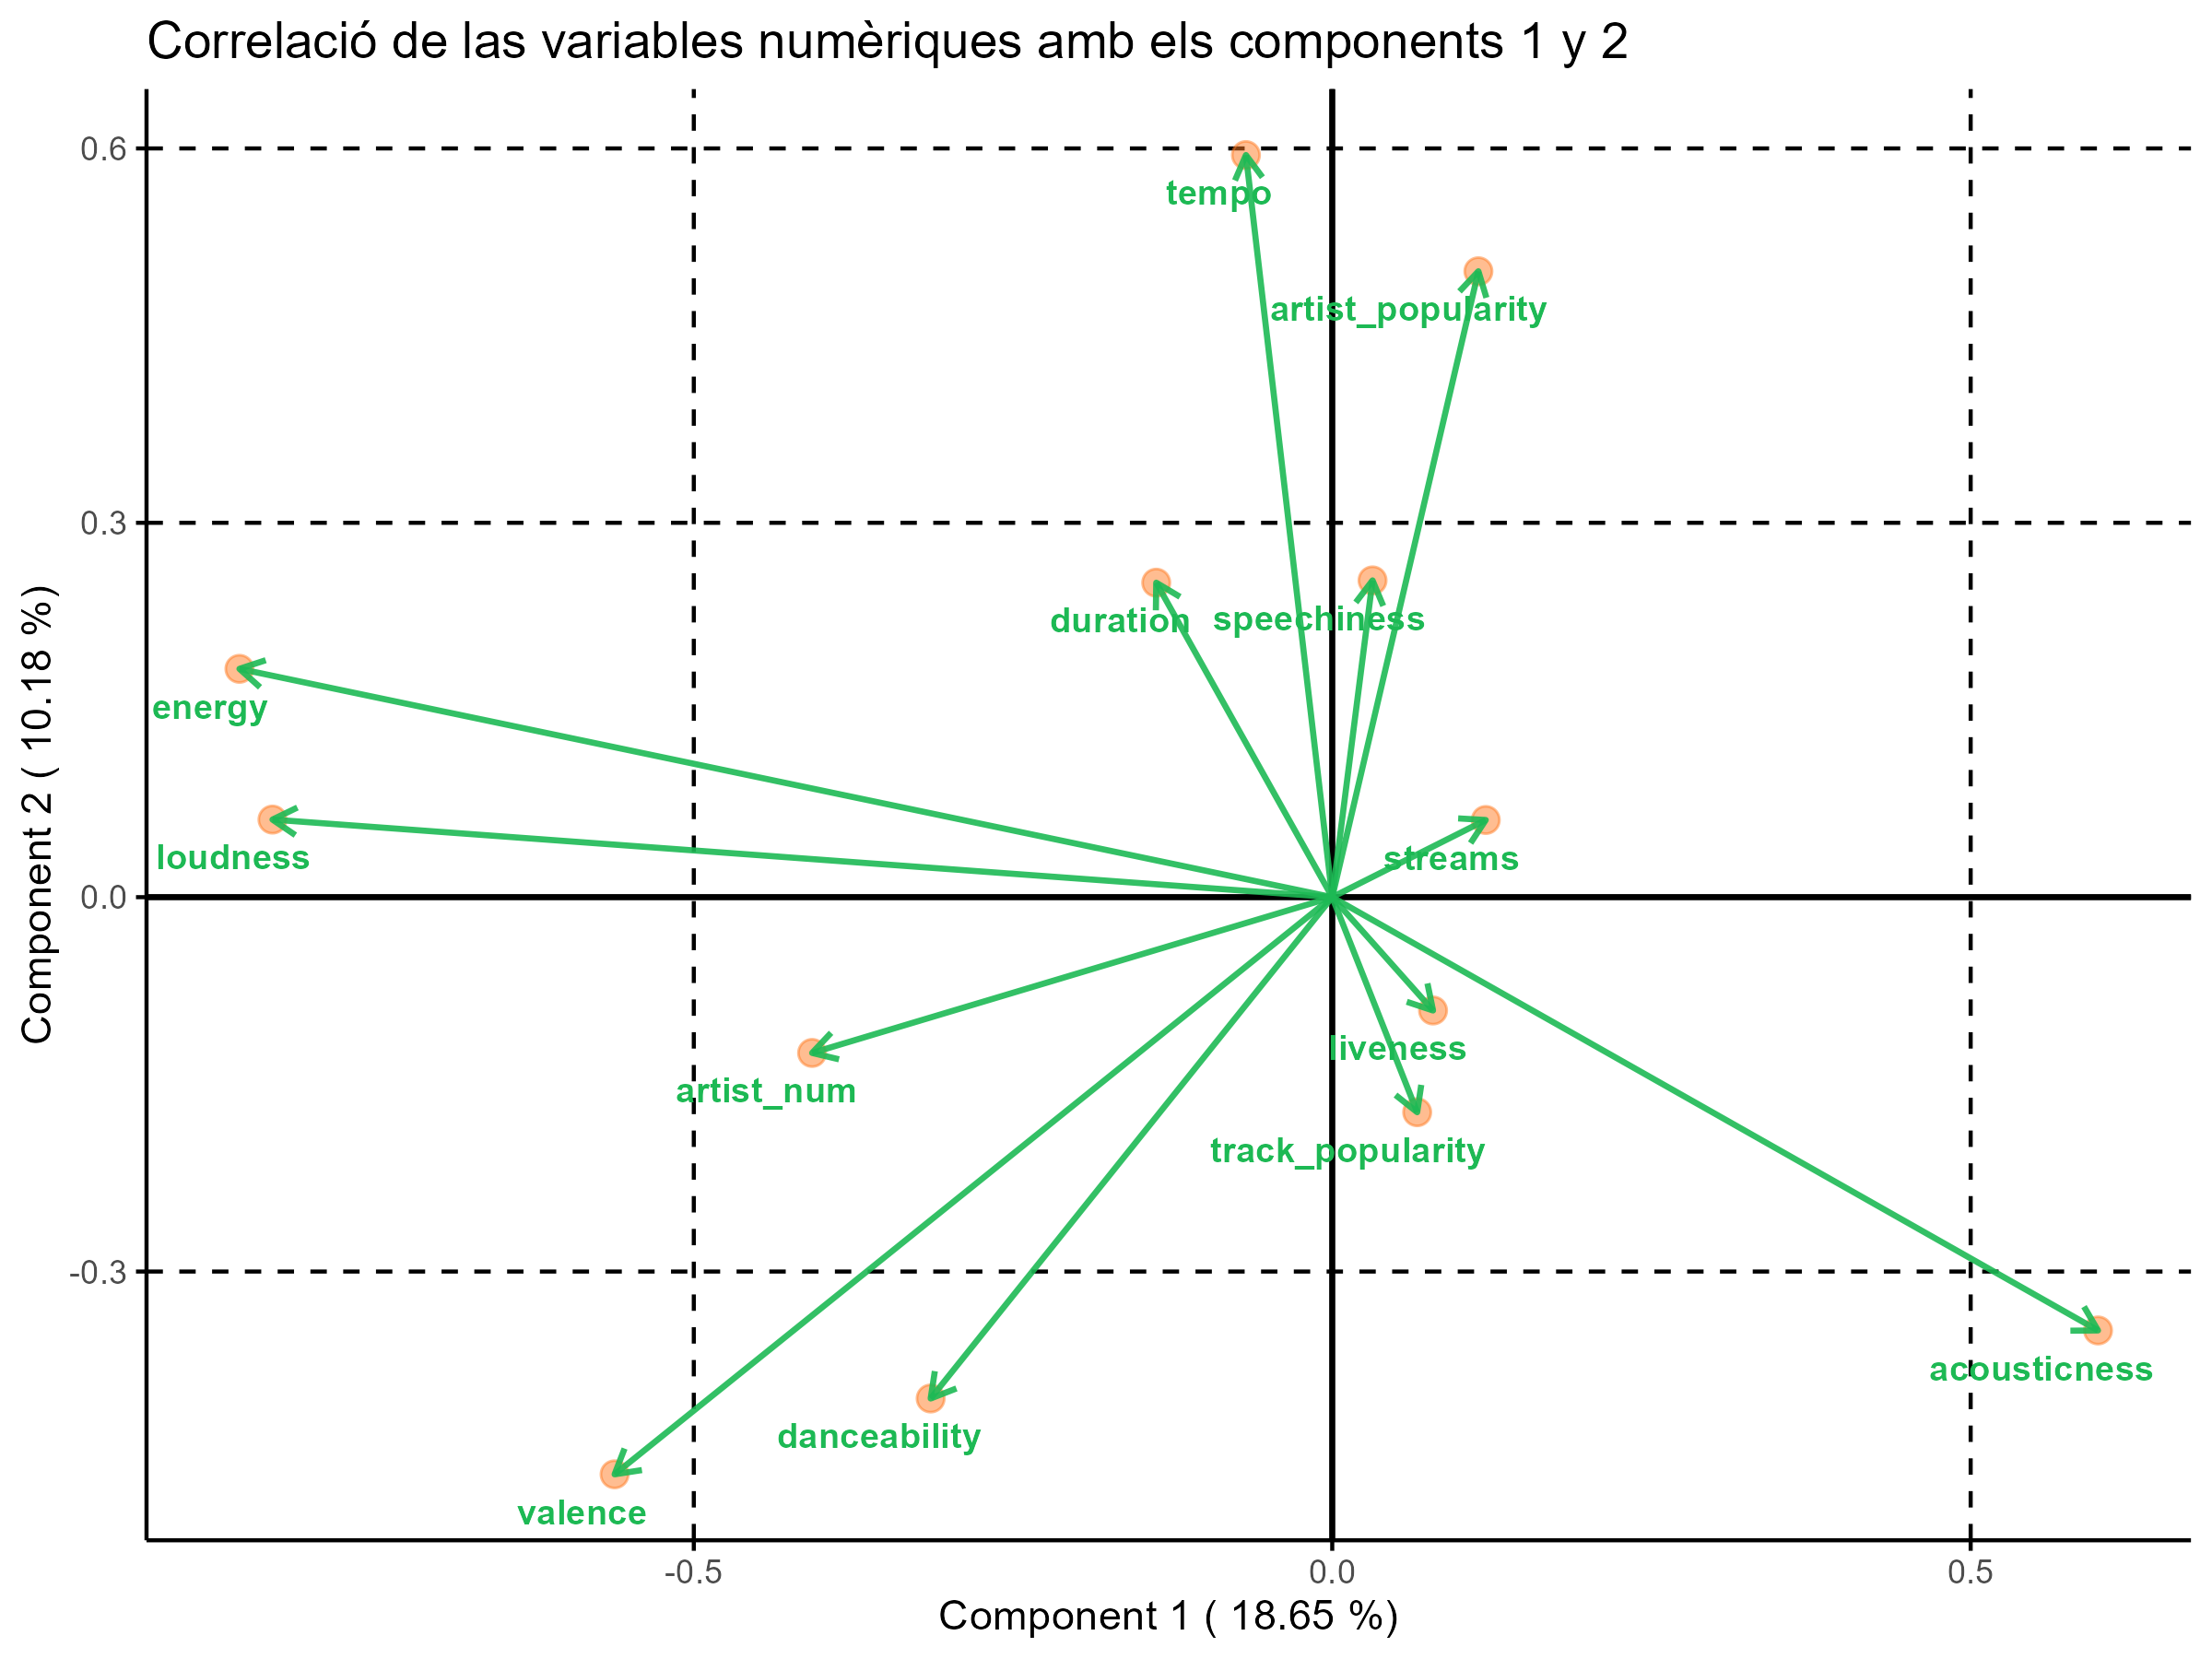
\includegraphics[width=0.8\linewidth]{Images/6_Factorial_Methods/ACP/Num_C1_C2.png}
    \caption{Variables numèriques projectades sobre els components 1 i 2}
    \label{fig:6_FM:ACP_C12}
\end{figure}

Pel que fa als components 3 i 4, en la figura \ref{fig:6_FM:ACP_C34} s'hi pot veure la seva projecció de les variables numèriques. El tercer component està altament correlacionat negativament amb les variables duration i artist\_num. Generalment, les cançons amb més artistes tendeixen a tenir una duració més llarga, ja que ha de donar temps a que tots els artistes puguin cantar. Per tant, el tercer component es pot dir que representa la durada de les cançons. Pel que fa al quart component, té una alta correlació negativa amb les variables speechiness i danceability, de manera que es pot dir que representa com de ballable és la lírica de les cançons.

\begin{figure}[H]
    \centering
    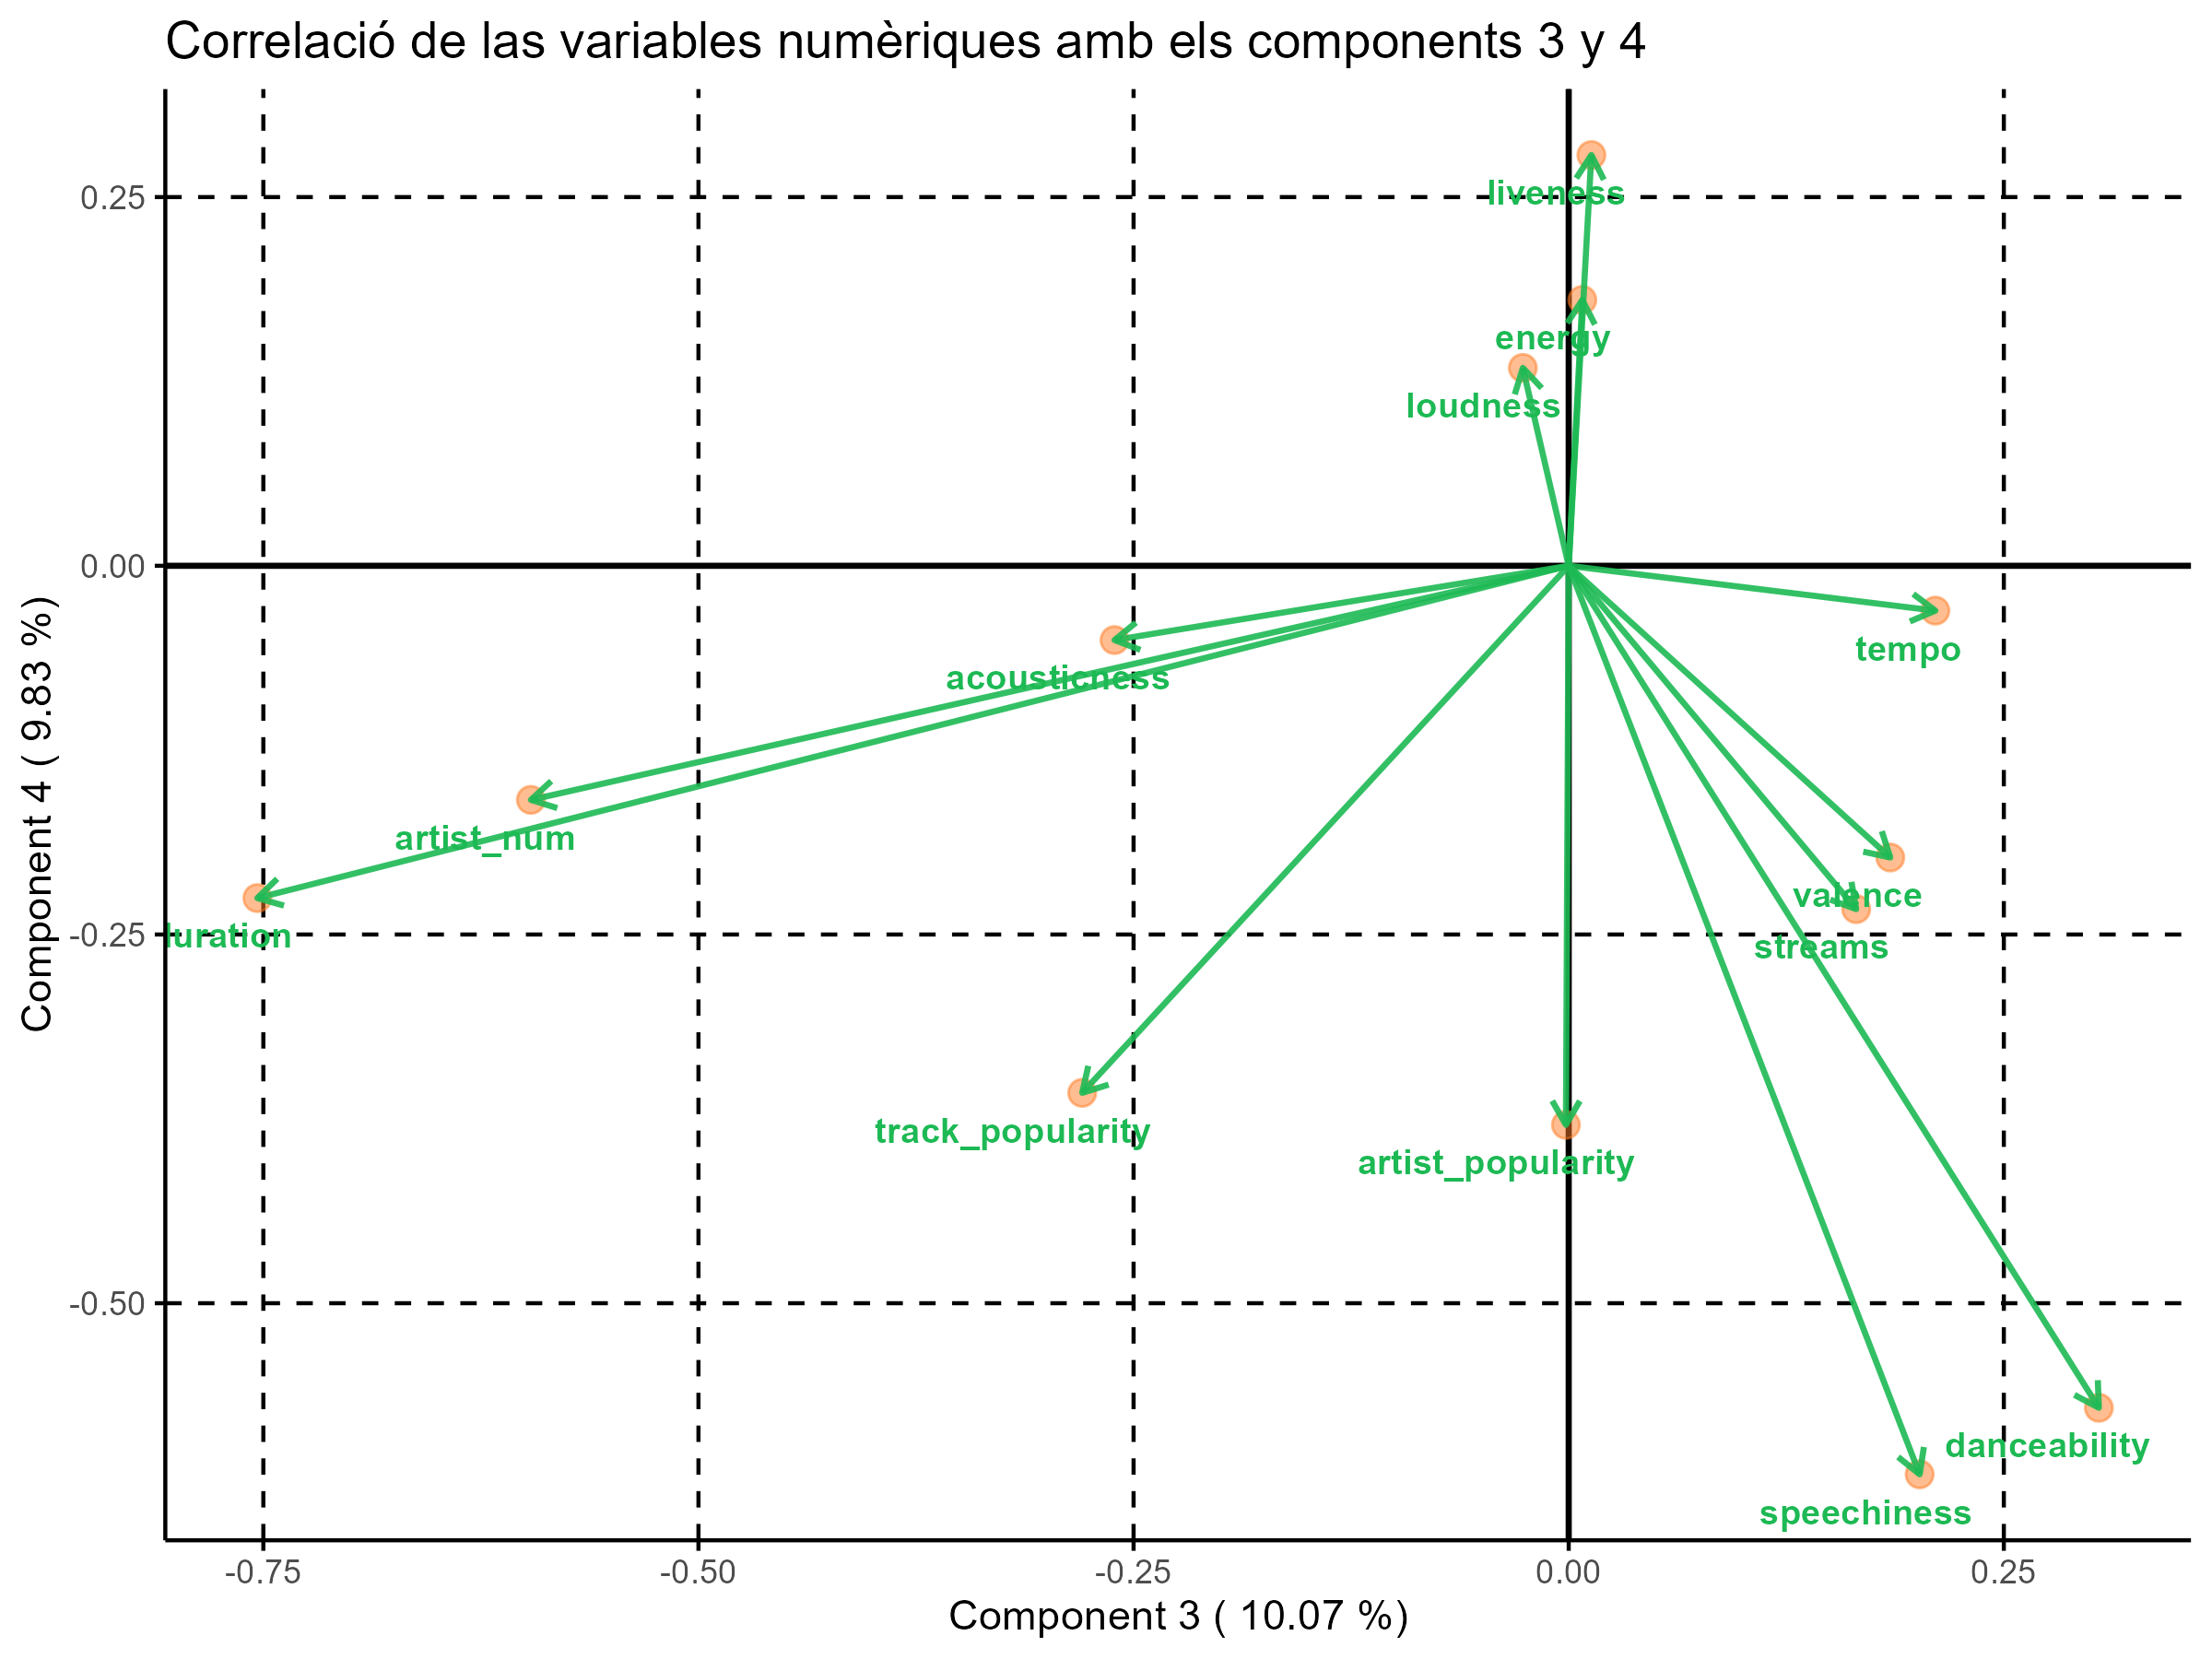
\includegraphics[width=0.8\linewidth]{Images/6_Factorial_Methods/ACP/Num_C3_C4.png}
    \caption{Variables numèriques projectades sobre els components 3 i 4}
    \label{fig:6_FM:ACP_C34}
\end{figure}

En la figura \ref{fig:6_FM:ACP_C56} es pot veure la projecció de les variables numèriques en els components 5 i 6. En el cinquè component, les variables artist\_popularity i streams tenen una forta correlació negativa, mentre que les variables speechiness i tempo hi tenen una correlació negativa. Això ens indica que el component 5 representa l'èxit de les cançons dels artistes depenent del seu gènere musical (ja que el gènere marca molt l'speechiness i el tempo de la cançó). Per altra banda, el component 6 està clarament correlacionat negativament amb la variable liveness, i també una mica amb streams, de manera que està relacionat amb el fet de que les cançons hagin estat gravades en grans concerts en directe.

\begin{figure}[H]
    \centering
    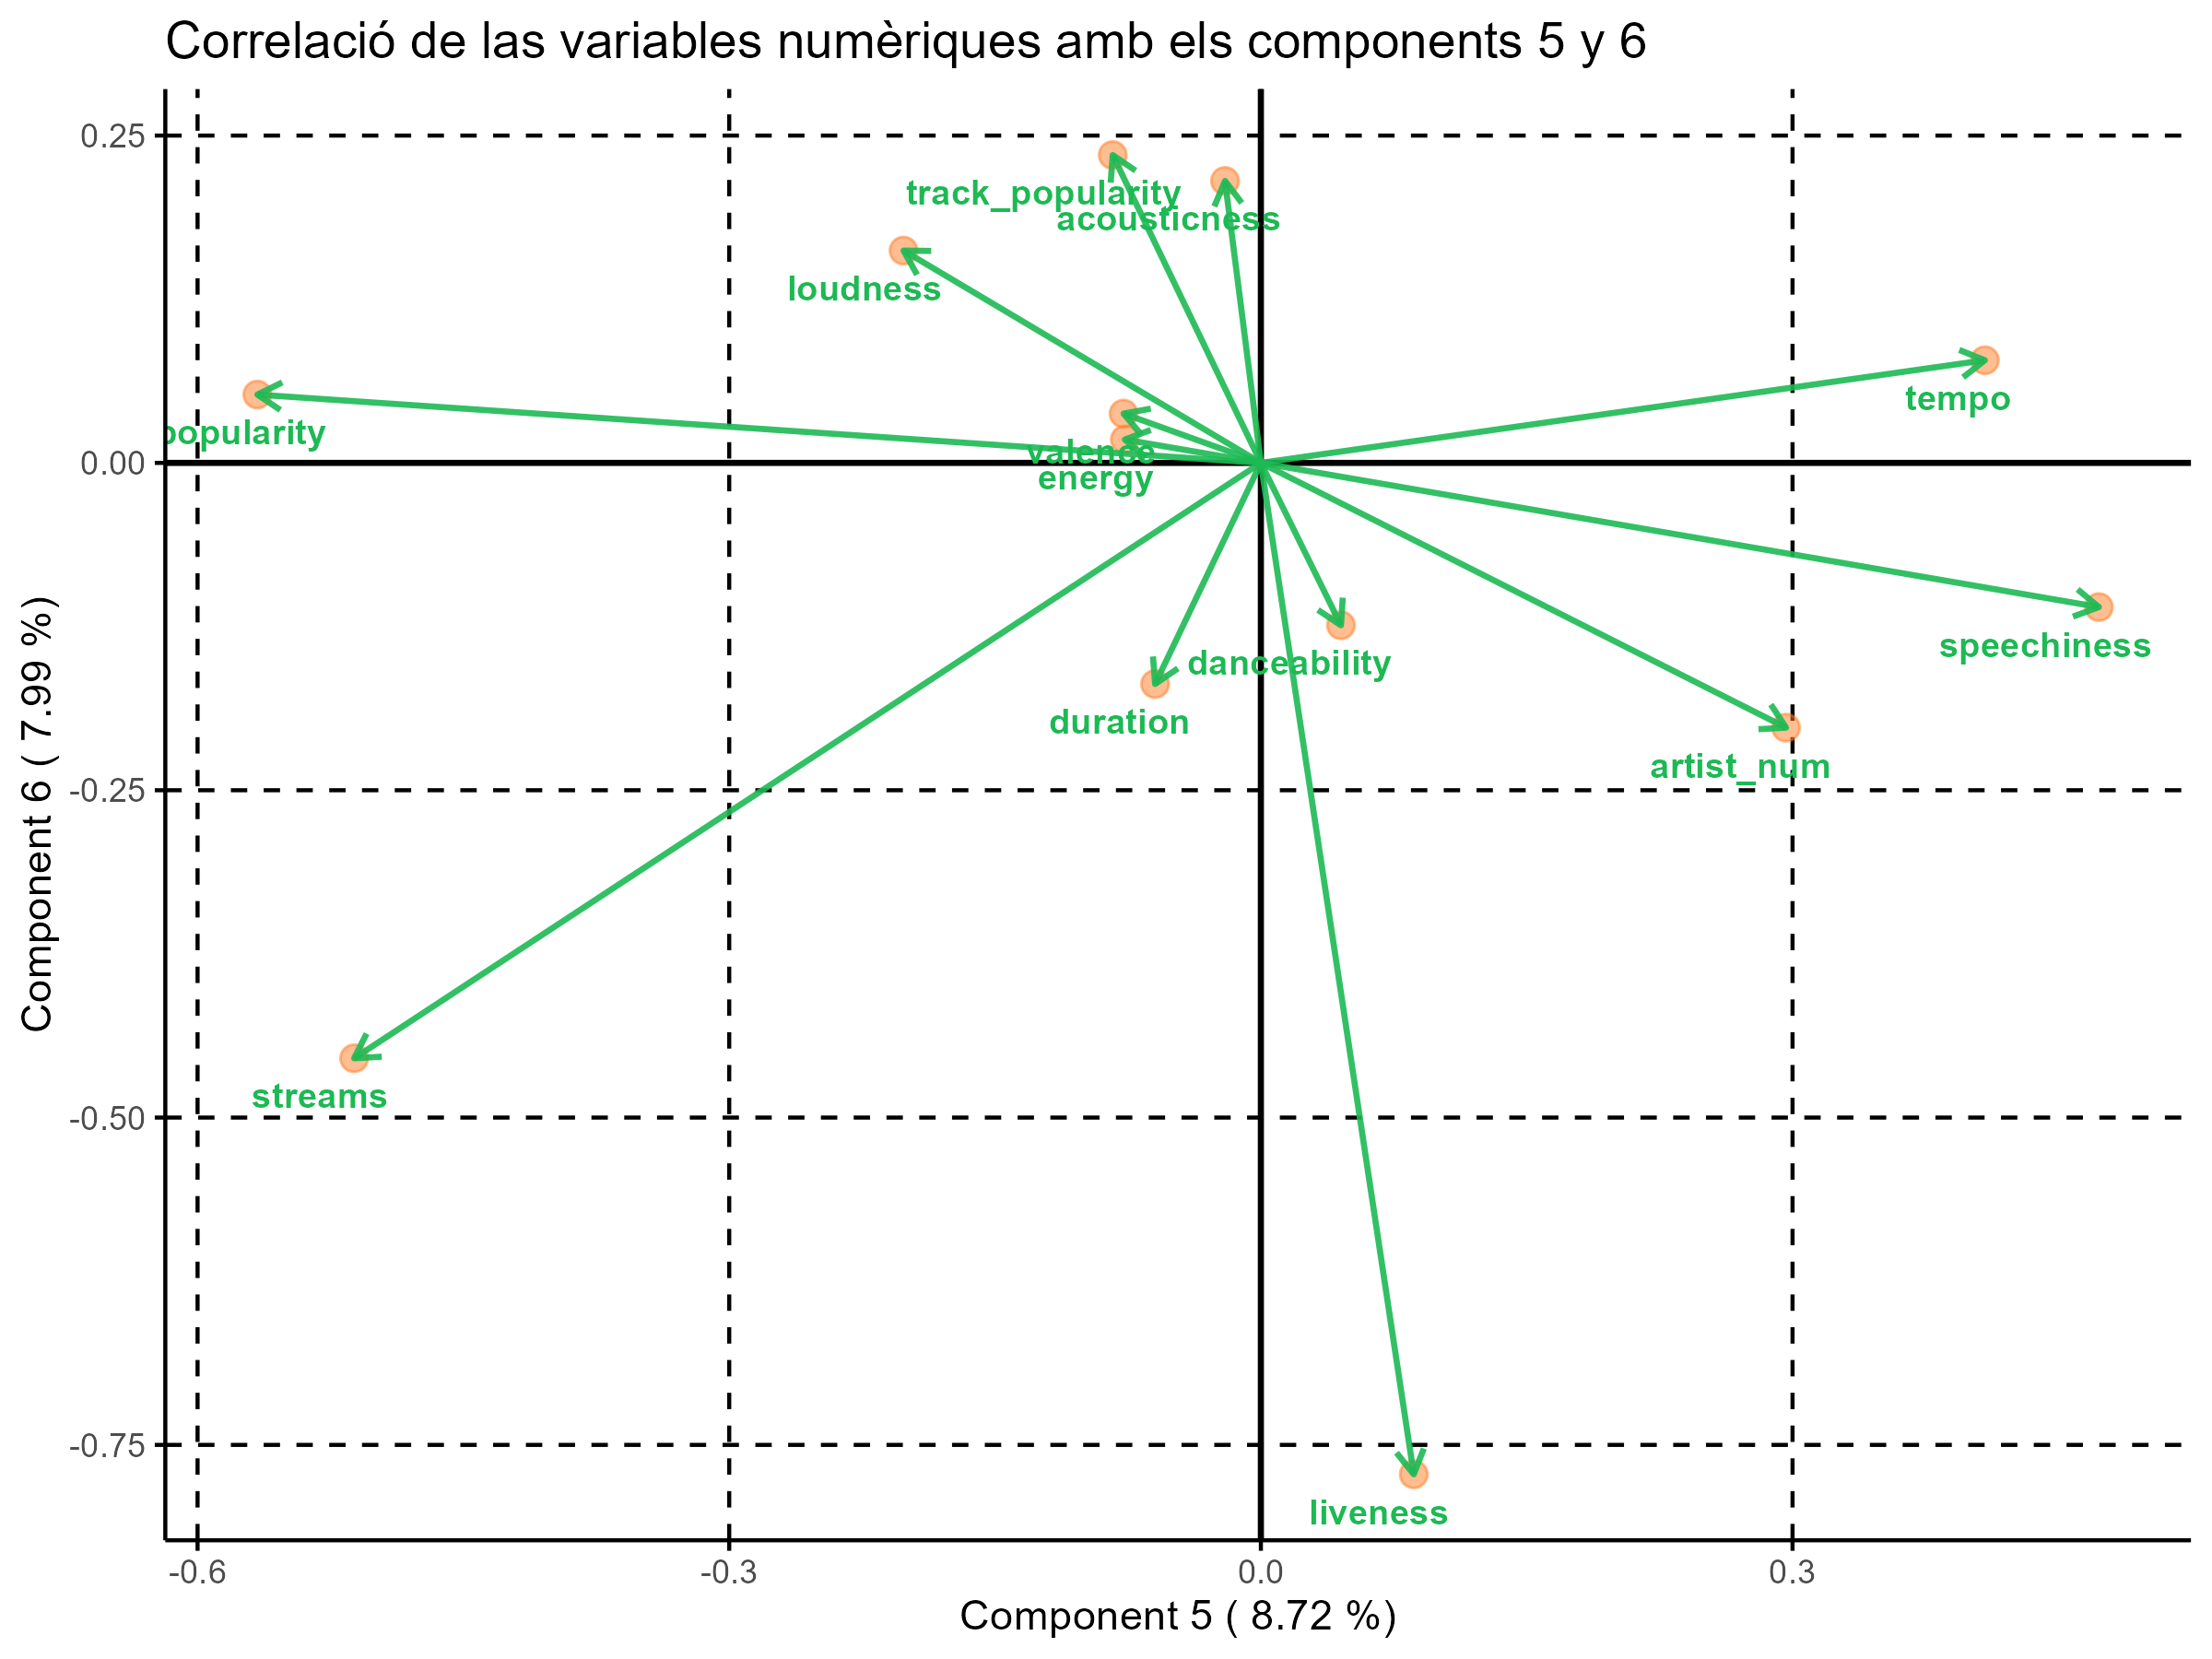
\includegraphics[width=0.8\linewidth]{Images/6_Factorial_Methods/ACP/Num_C5_C6.png}
    \caption{Variables numèriques projectades sobre els components 5 i 6}
    \label{fig:6_FM:ACP_C56}
\end{figure}

En la figura \ref{fig:6_FM:ACP_C78} es poden veure les variables numèriques projectades sobre els components 7 i 8. Clarament, el component y té una altra correlació amb la variable track\_popularity, de manera que representa la popularitat de la cançó al final del registre de la base de dades (ja que les dades de track\_popularity en la base de dades d'aquest projecte han estat mesurades en la última setmana del seu registre). No obstant, el component 8 té una forta correlació negativa amb les variables streams i tempo, de manera que pot representar l'èxit que ha tingut una cançó depenent del seu ritme (similar al component 5).

\begin{figure}[H]
    \centering
    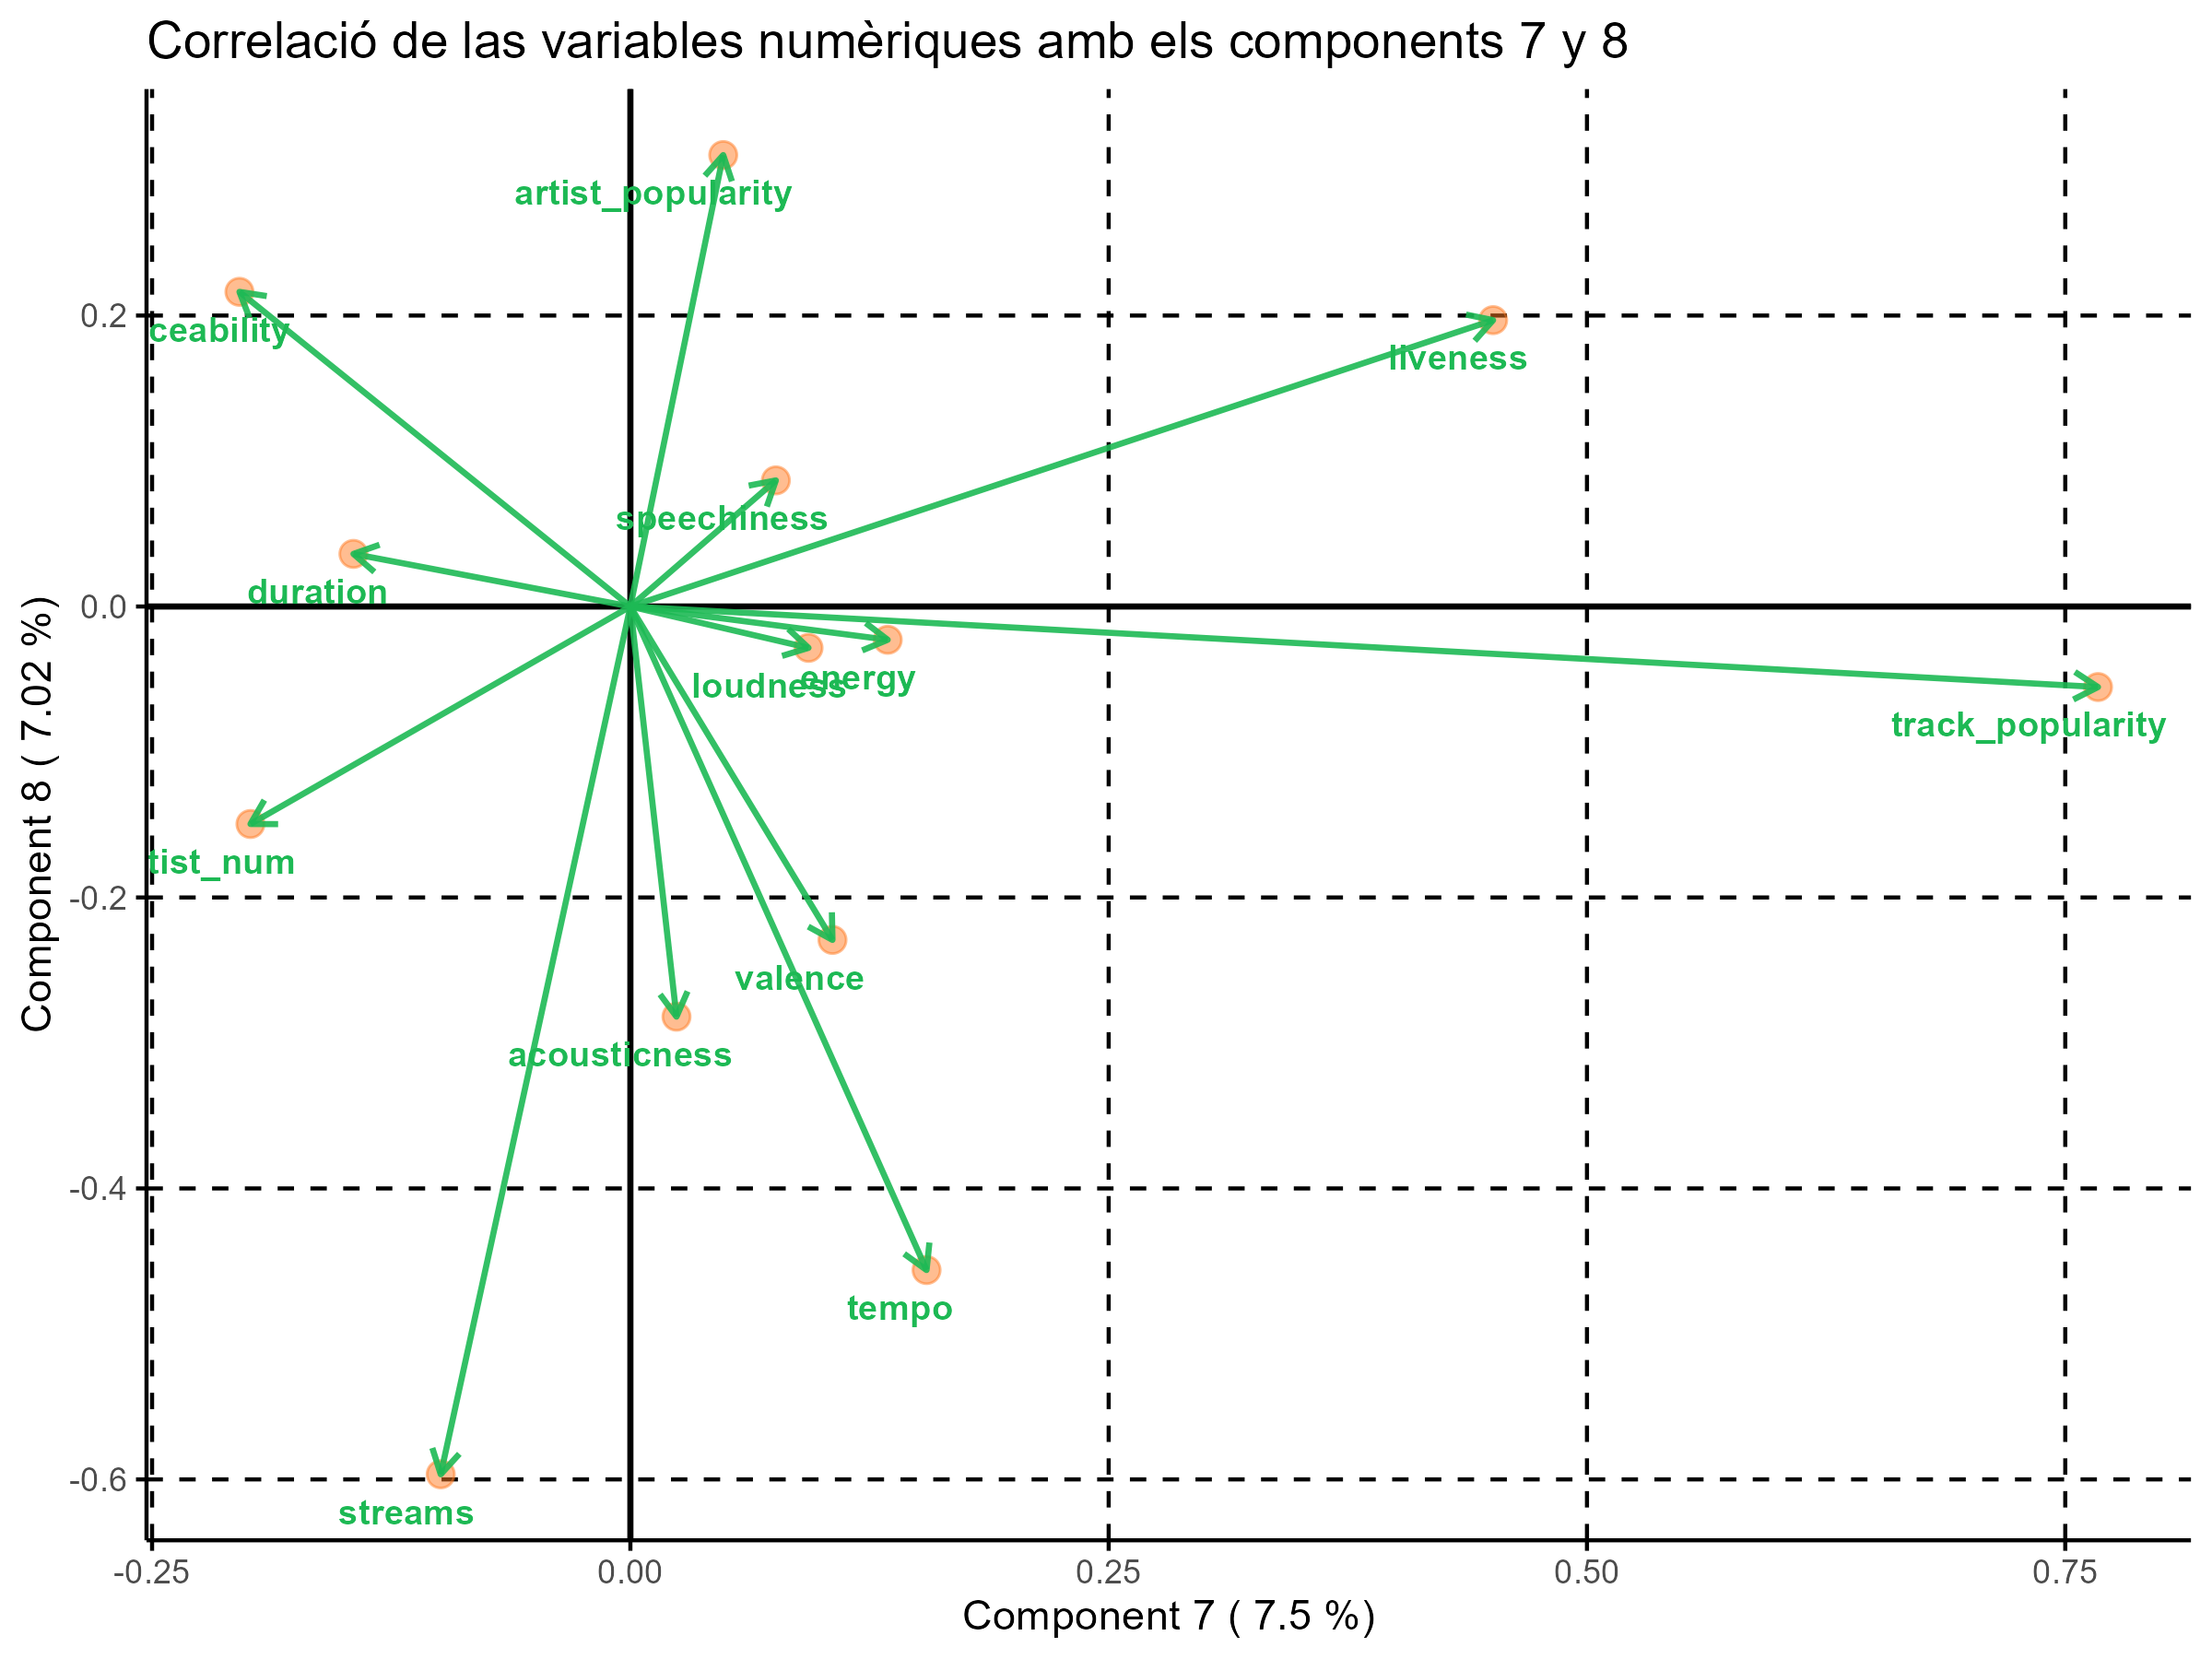
\includegraphics[width=0.8\linewidth]{Images/6_Factorial_Methods/ACP/Num_C7_C8.png}
    \caption{Variables numèriques projectades sobre els components 7 i 8}
    \label{fig:6_FM:ACP_C78}
\end{figure}

Finalment, en la figura \ref{fig:6_FM:ACP_C19} es poden veure les projeccions de les variables numèriques a sobre dels components 1 i 9. El primer component ja ha estat analitzat, però el component 9 ens indica una certa correlació positiva amb les variables acousticness i valence, de manera que es pot dir que representa característiques sobre la musicalitat de les cançons.

\begin{figure}[H]
    \centering
    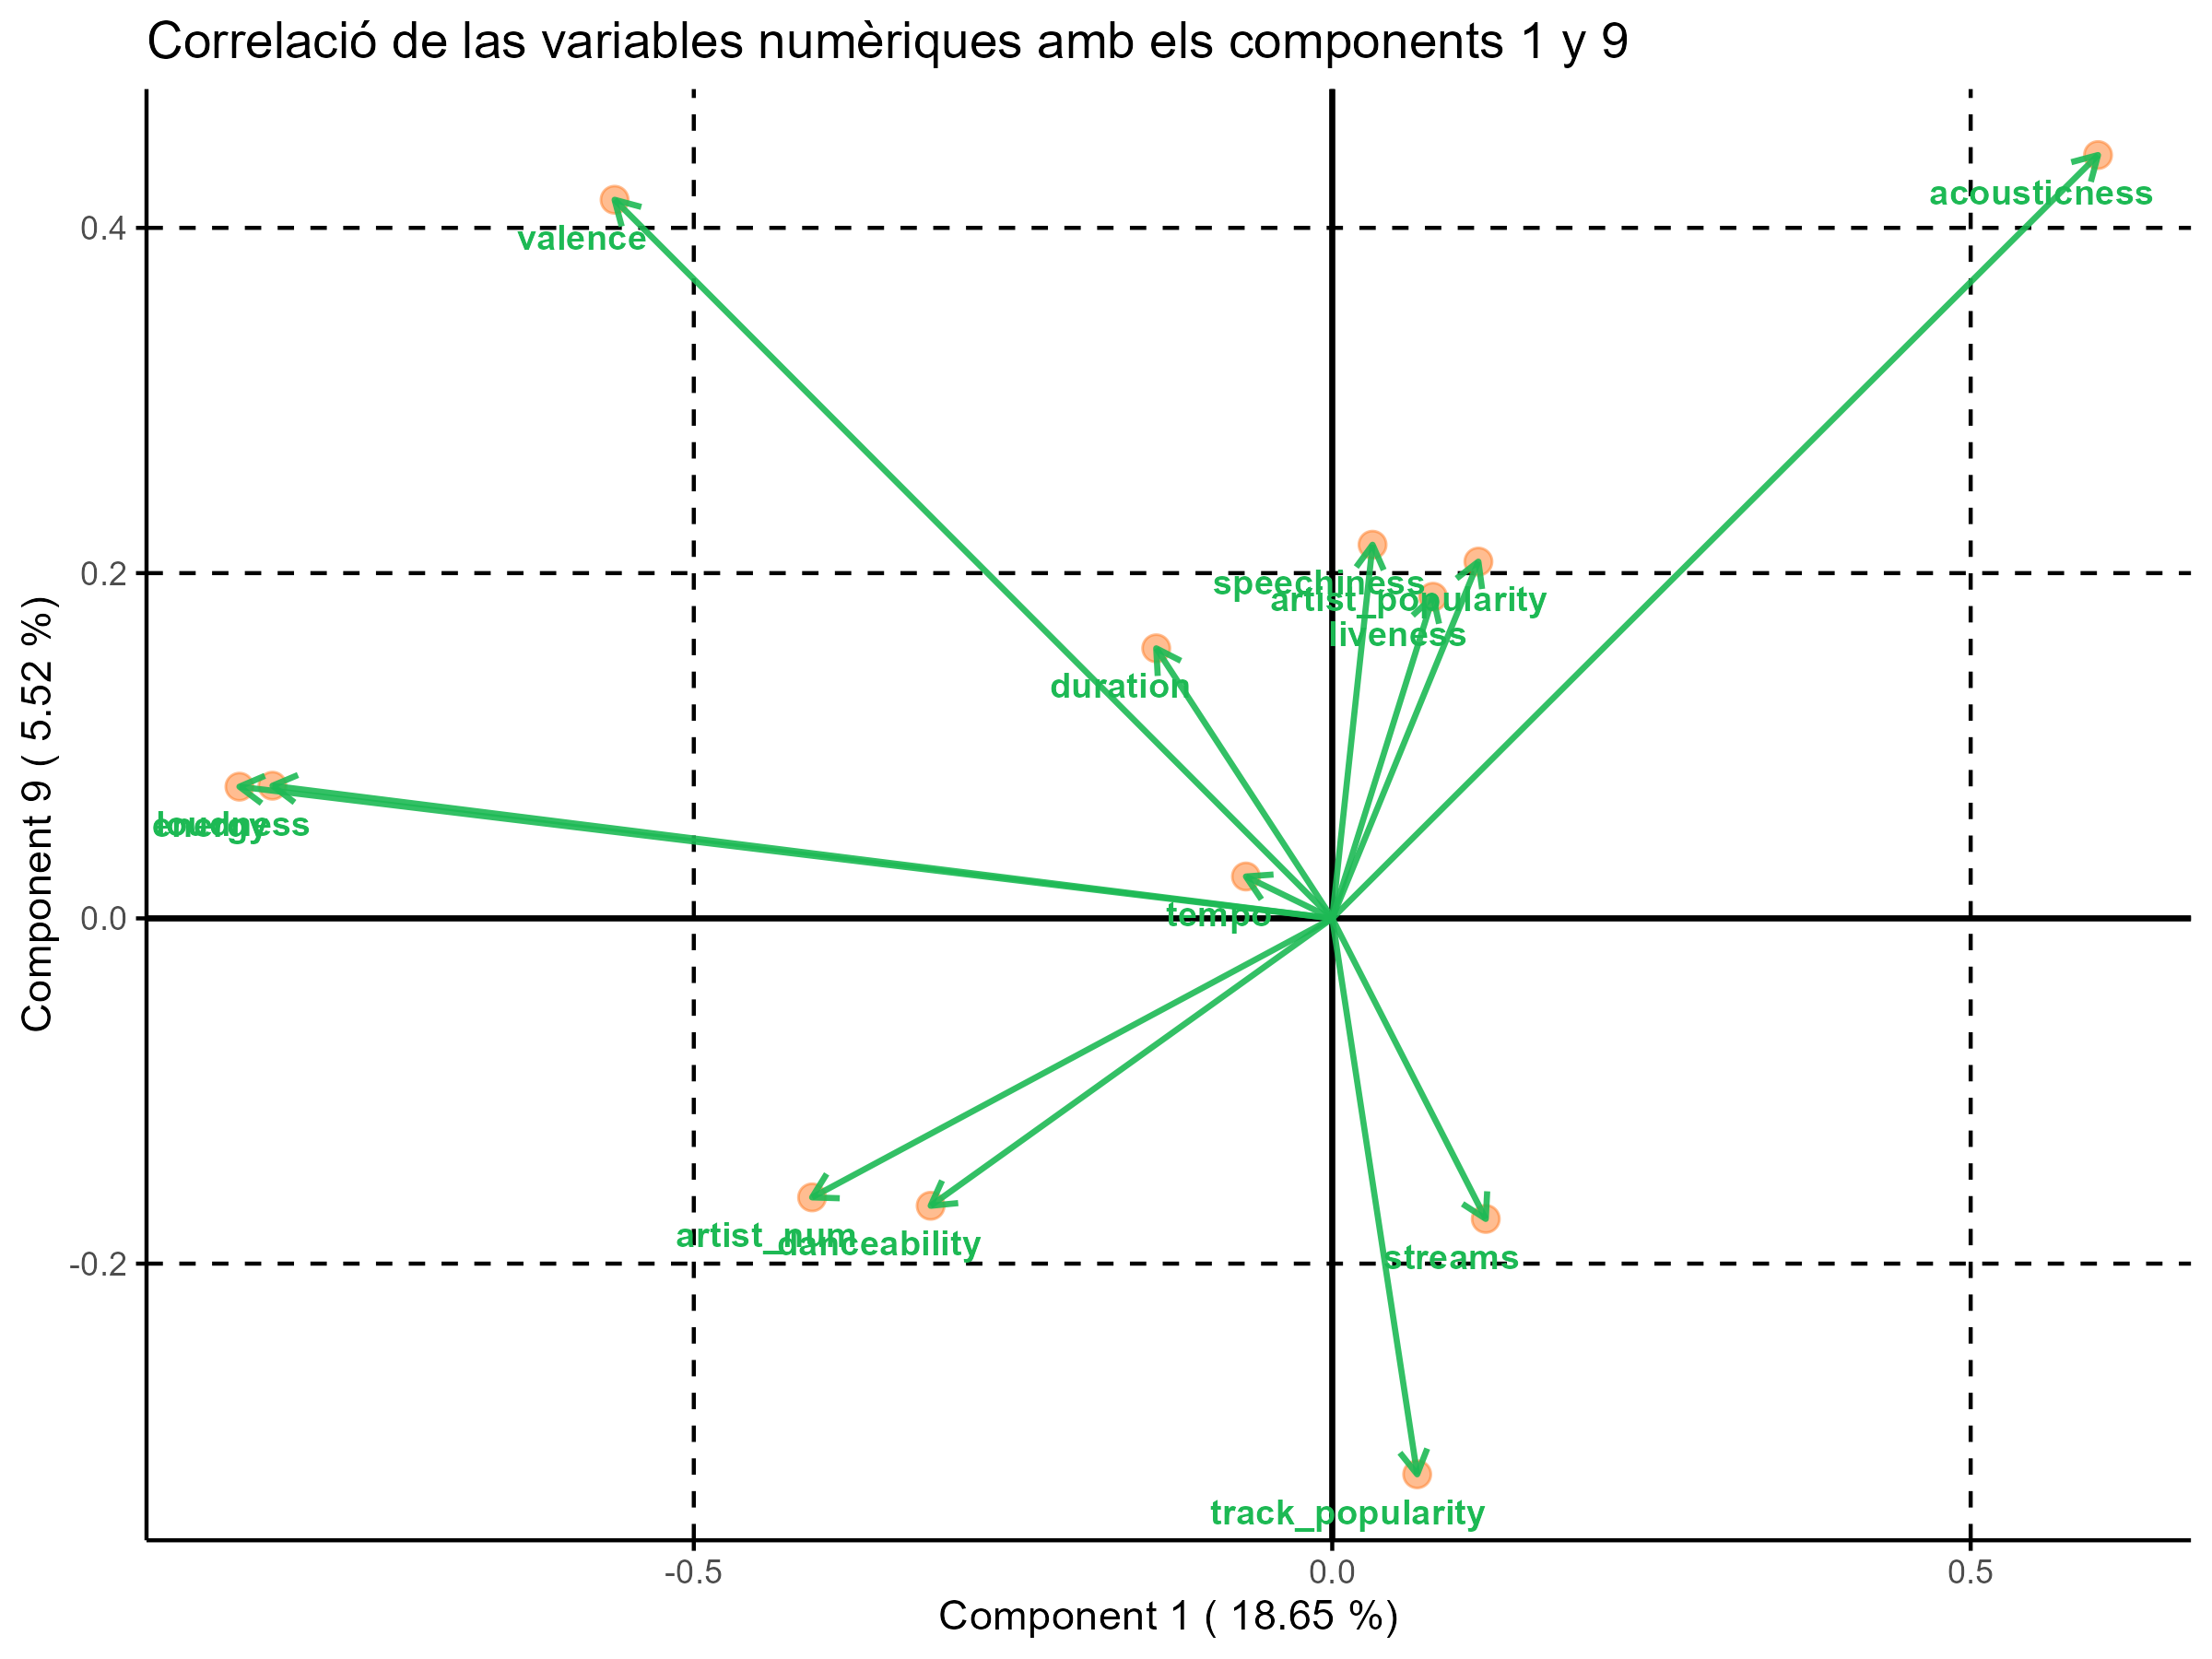
\includegraphics[width=0.8\linewidth]{Images/6_Factorial_Methods/ACP/Num_C1_C9.png}
    \caption{Variables numèriques projectades sobre els components 1 i 9}
    \label{fig:6_FM:ACP_C19}
\end{figure}

\subsubsection{Variables categòriques}
Una vegada ja s'han analitzat les variables numèriques amb els diferents components, s'han projectat els centroides de les diferents classes de cada variable categòrica en els components 1 i 2 (els que expliquen major percentatge de variància) per tal de comparar-los amb els components i extreure conclusions sobre la base de dades. En la figura \ref{fig:6_FM:ACP_all_cat} es poden veure tots aquests centroides projectats per les variables que han mostrat ser més rellevants (collab, latino, christmas, nationality i time\_signature). No obstant, a continuació s'analitzaran variable per variable.

\begin{figure}[H]
    \centering
    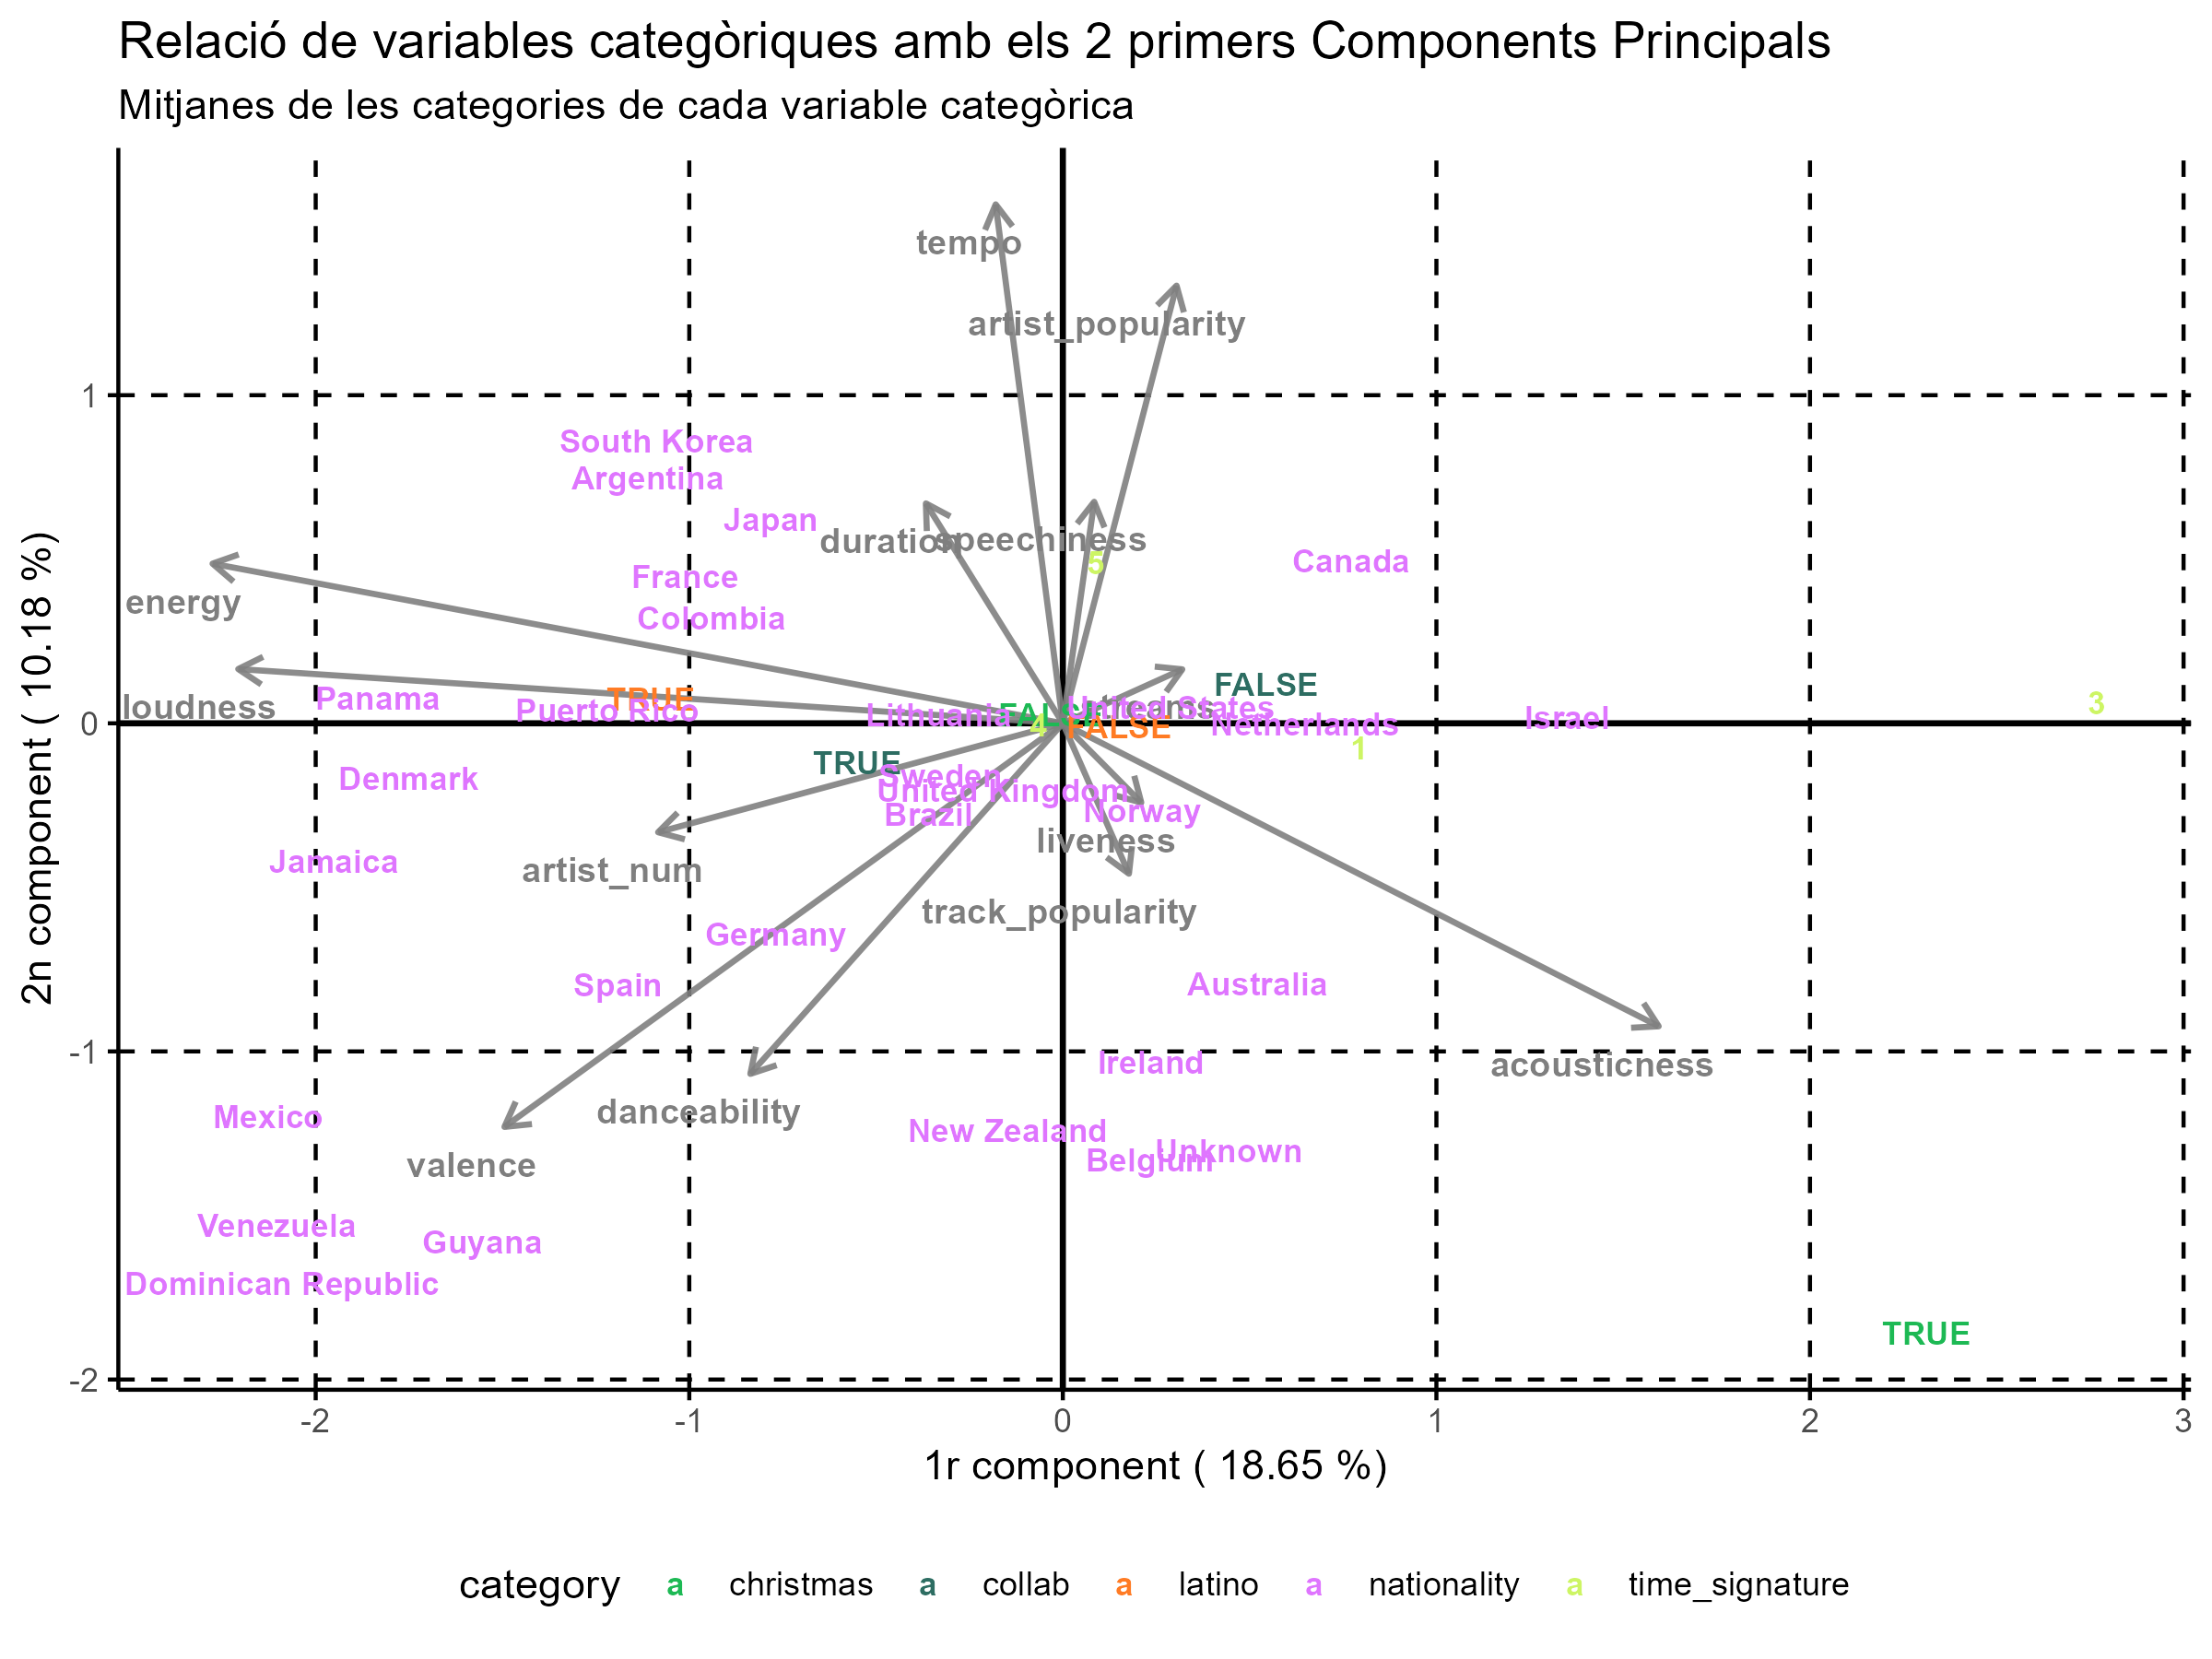
\includegraphics[width=0.8\linewidth]{Images/6_Factorial_Methods/ACP/All_Cat_C1_C2_nationality.png}
    \caption{Centroides de les classes de les 5 variables categòriques que permeten extreure millors conclusions projectades sobre els components 1 i 2}
    \label{fig:6_FM:ACP_all_cat}
\end{figure}

En la figura \ref{fig:6_FM:ACP_collab} es pot veure com el centroide de la classe TRUE es troba separat del de la classe FALSE. Observant les variables numèriques i els eixos es pot concloure que les cançons amb colaboracions de diferents artistes acostumen a tenir una major danceability i valence.

\begin{figure}[H]
    \centering
    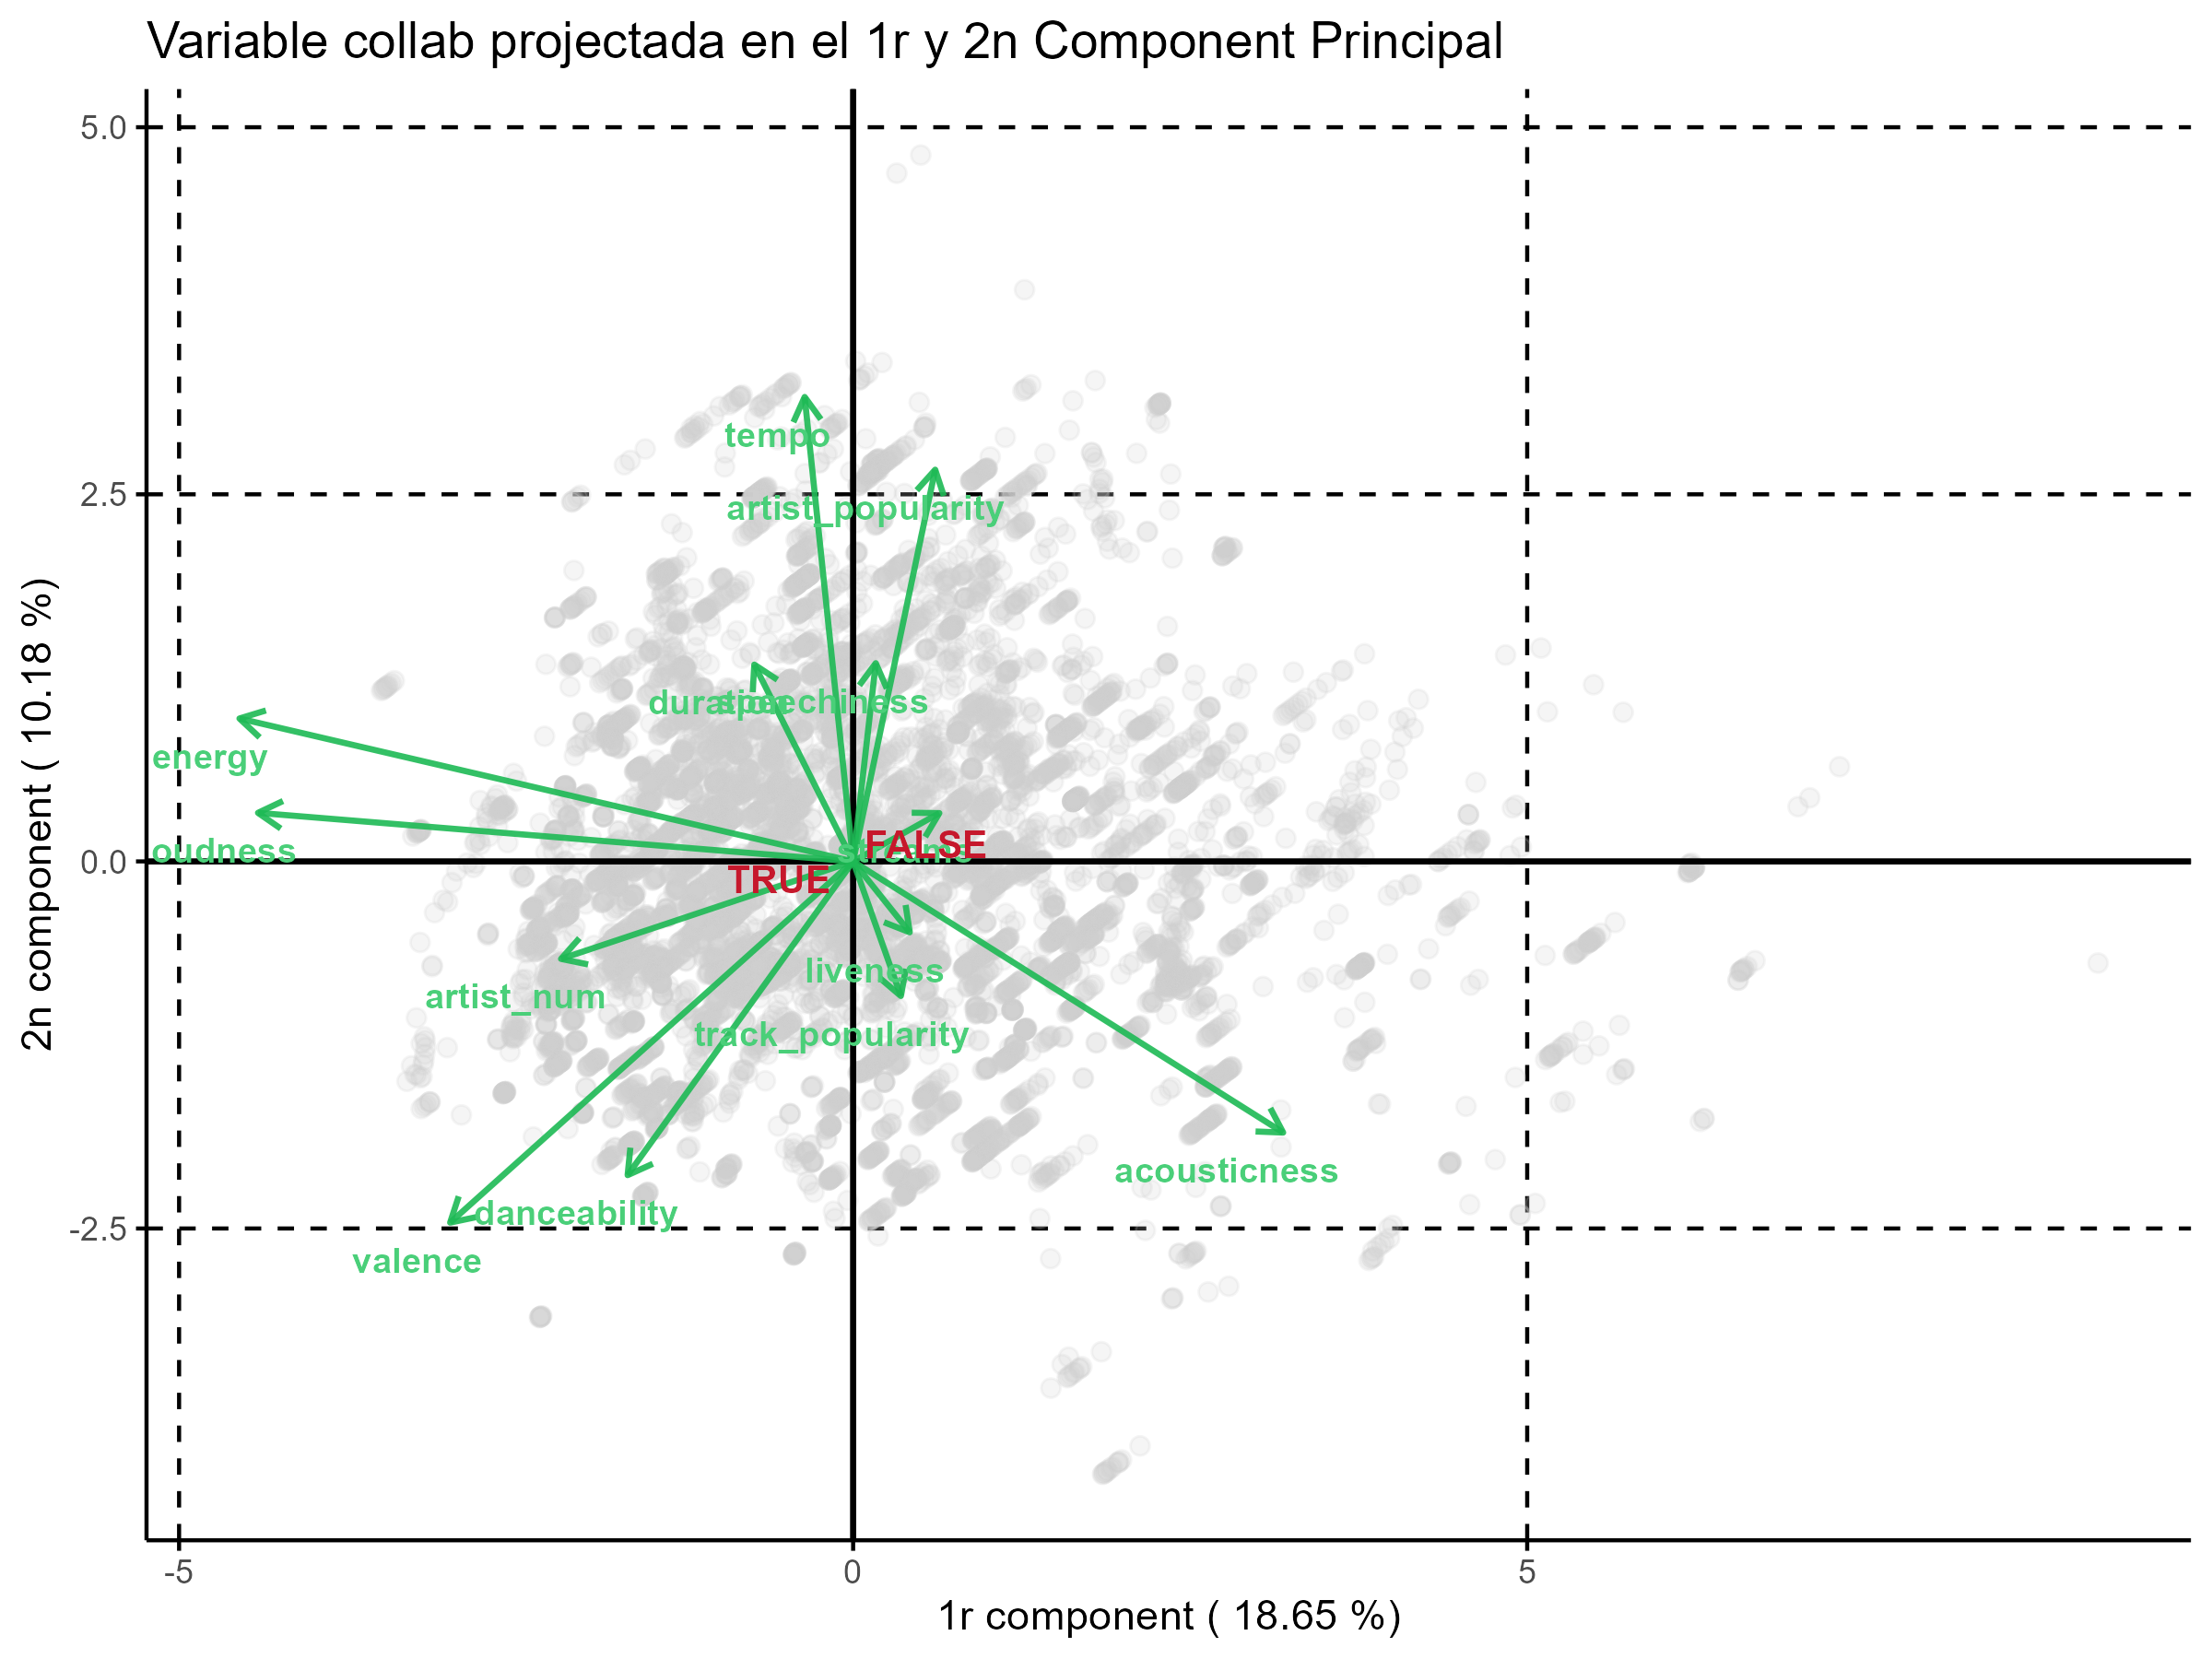
\includegraphics[width=0.6\linewidth]{Images/6_Factorial_Methods/ACP/Cat_C1_C2_collab.png}
    \caption{Centroides de les classes de la variable collab projectats en els components 1 i 2}
    \label{fig:6_FM:ACP_collab}
\end{figure}

Pel que fa a la variable latino, la projecció dels seus centroides es pot veure en la figura \ref{fig:6_FM:ACP_latino}. Està clar que les cançons d'aquest gènere tenen una major energy i loudness, de manera que tenen més ``potència''.

\begin{figure}[H]
    \centering
    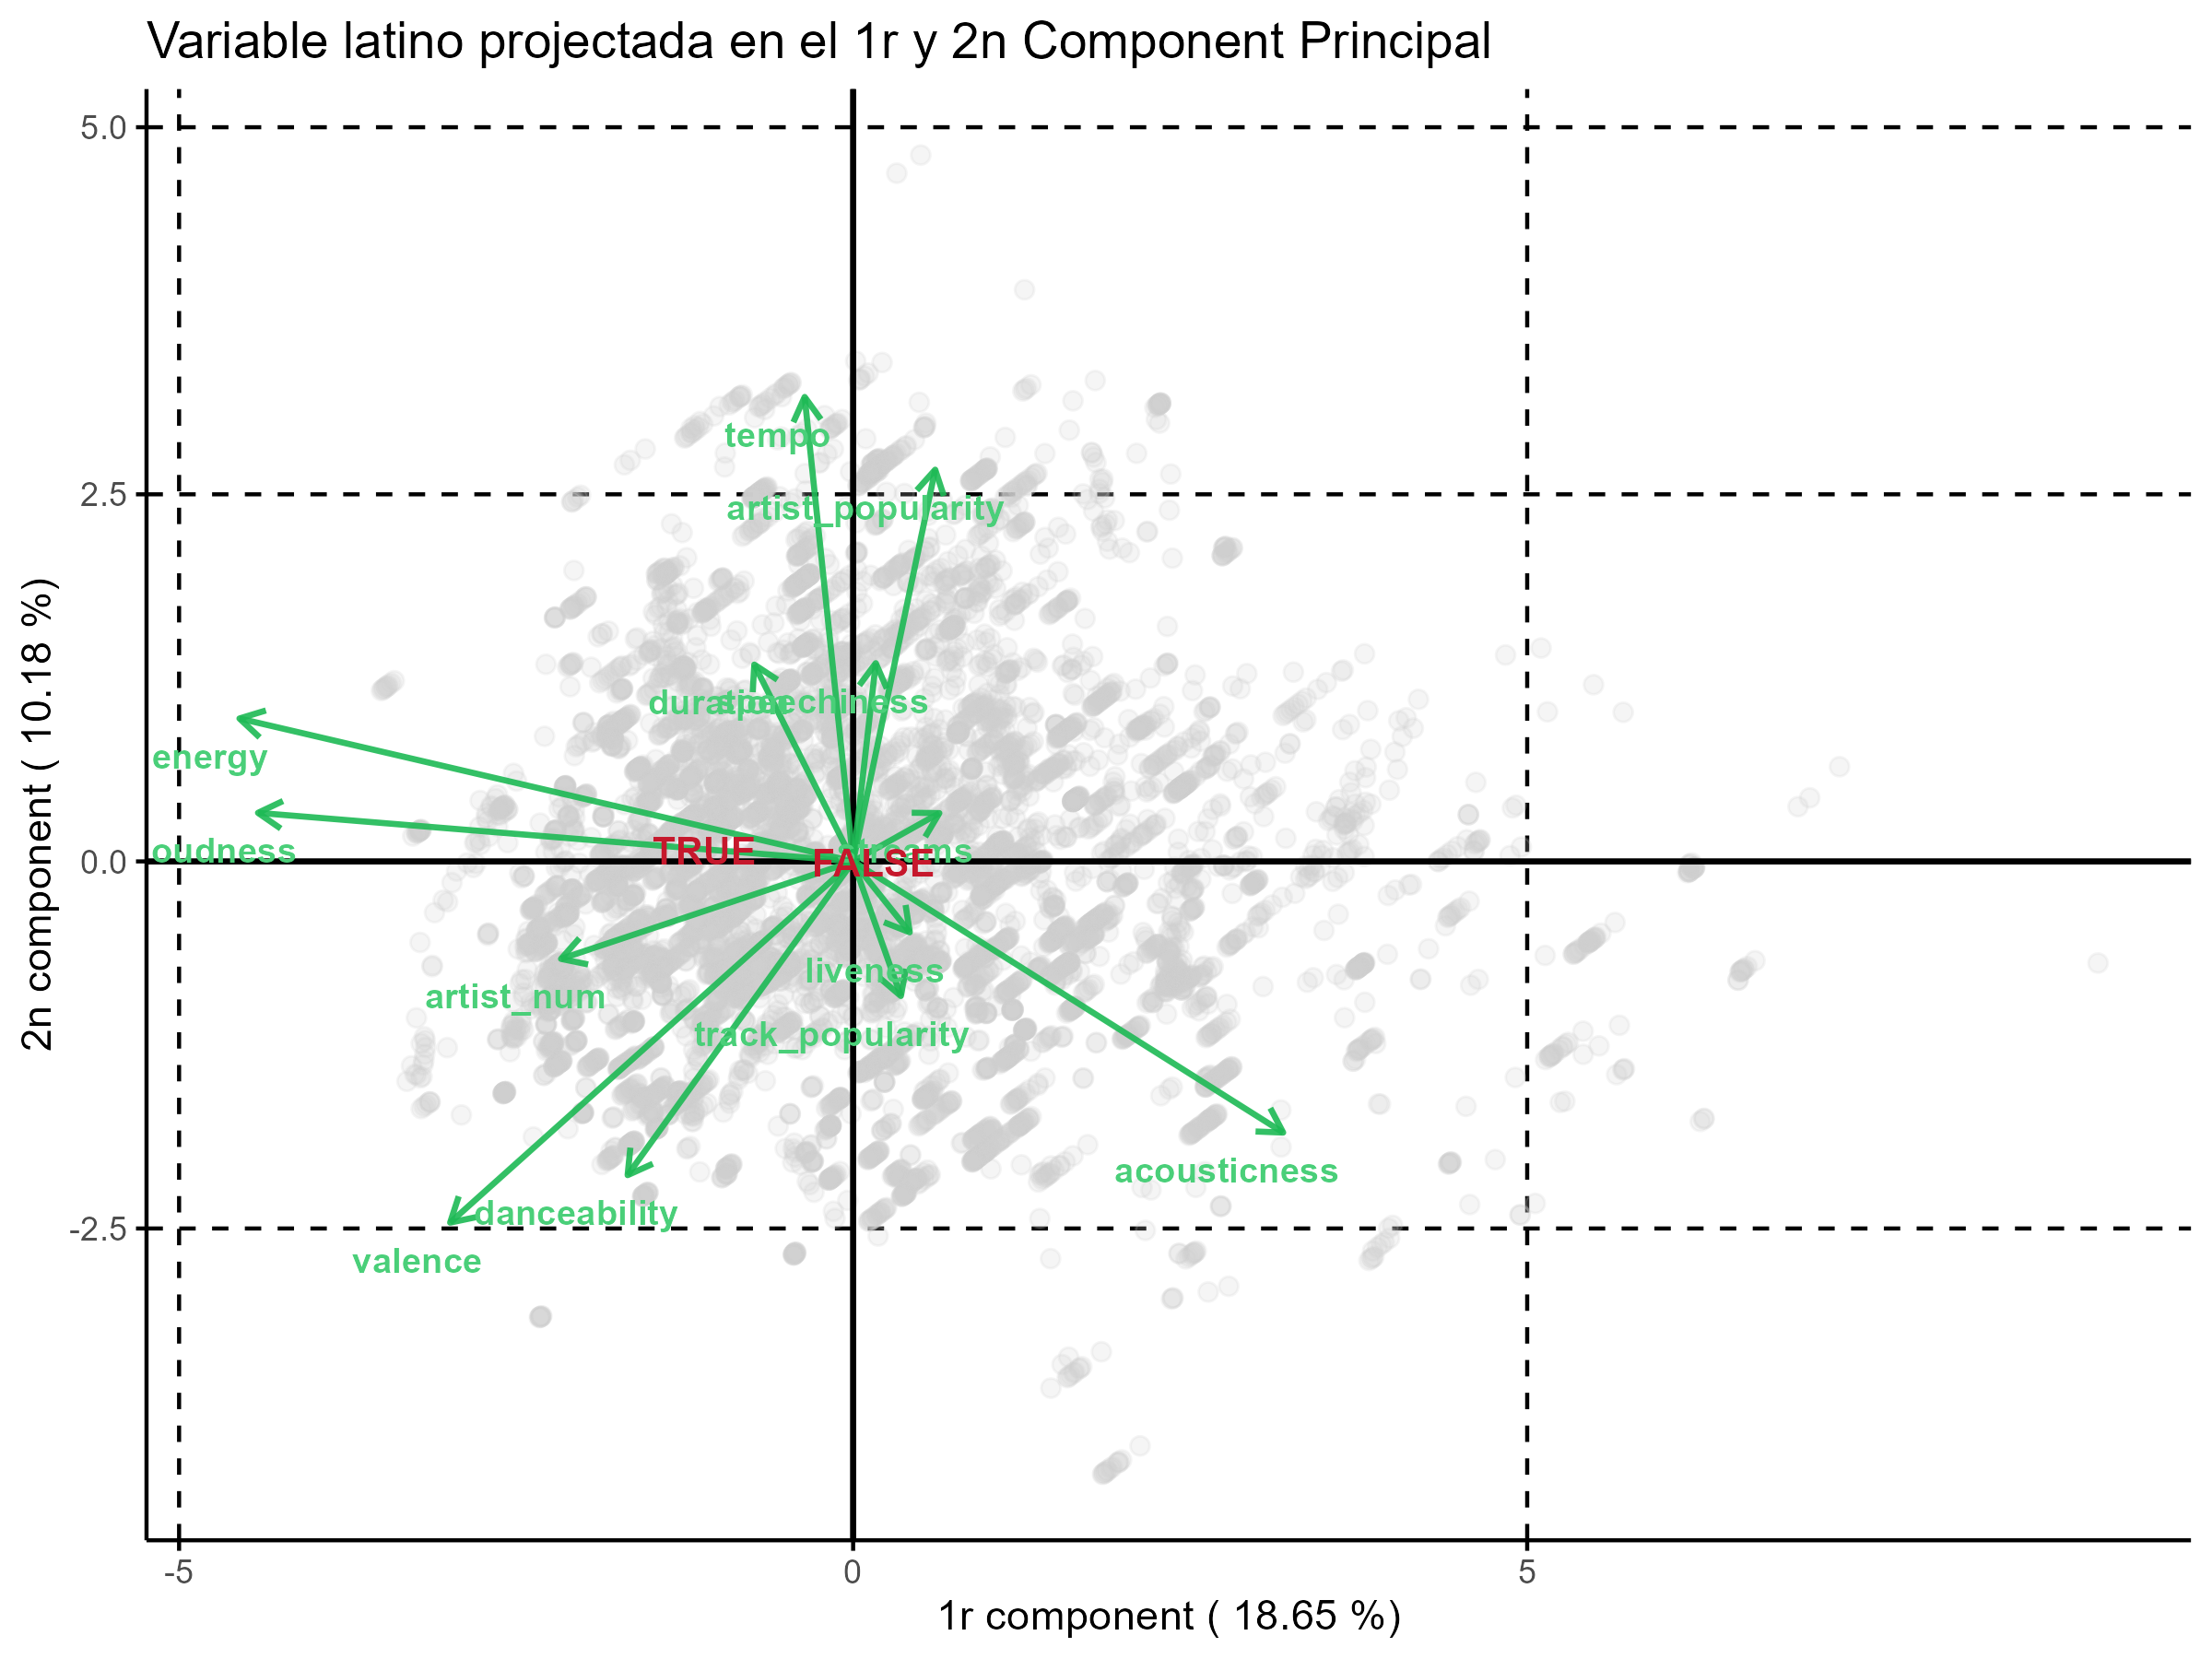
\includegraphics[width=0.6\linewidth]{Images/6_Factorial_Methods/ACP/Cat_C1_C2_latino.png}
    \caption{Centroides de les classes de la variable latino projectats en els components 1 i 2}
    \label{fig:6_FM:ACP_latino}
\end{figure}

La variable christmas es pot observar en la figura \ref{fig:6_FM:ACP_christmas} i mostra de forma evident com les cançons de nadal tenen una alta correlació amb acousticness, de manera que acostumen a tenir menys lletra i més música amb instruments i sense tants elements electrònics.

\begin{figure}[H]
    \centering
    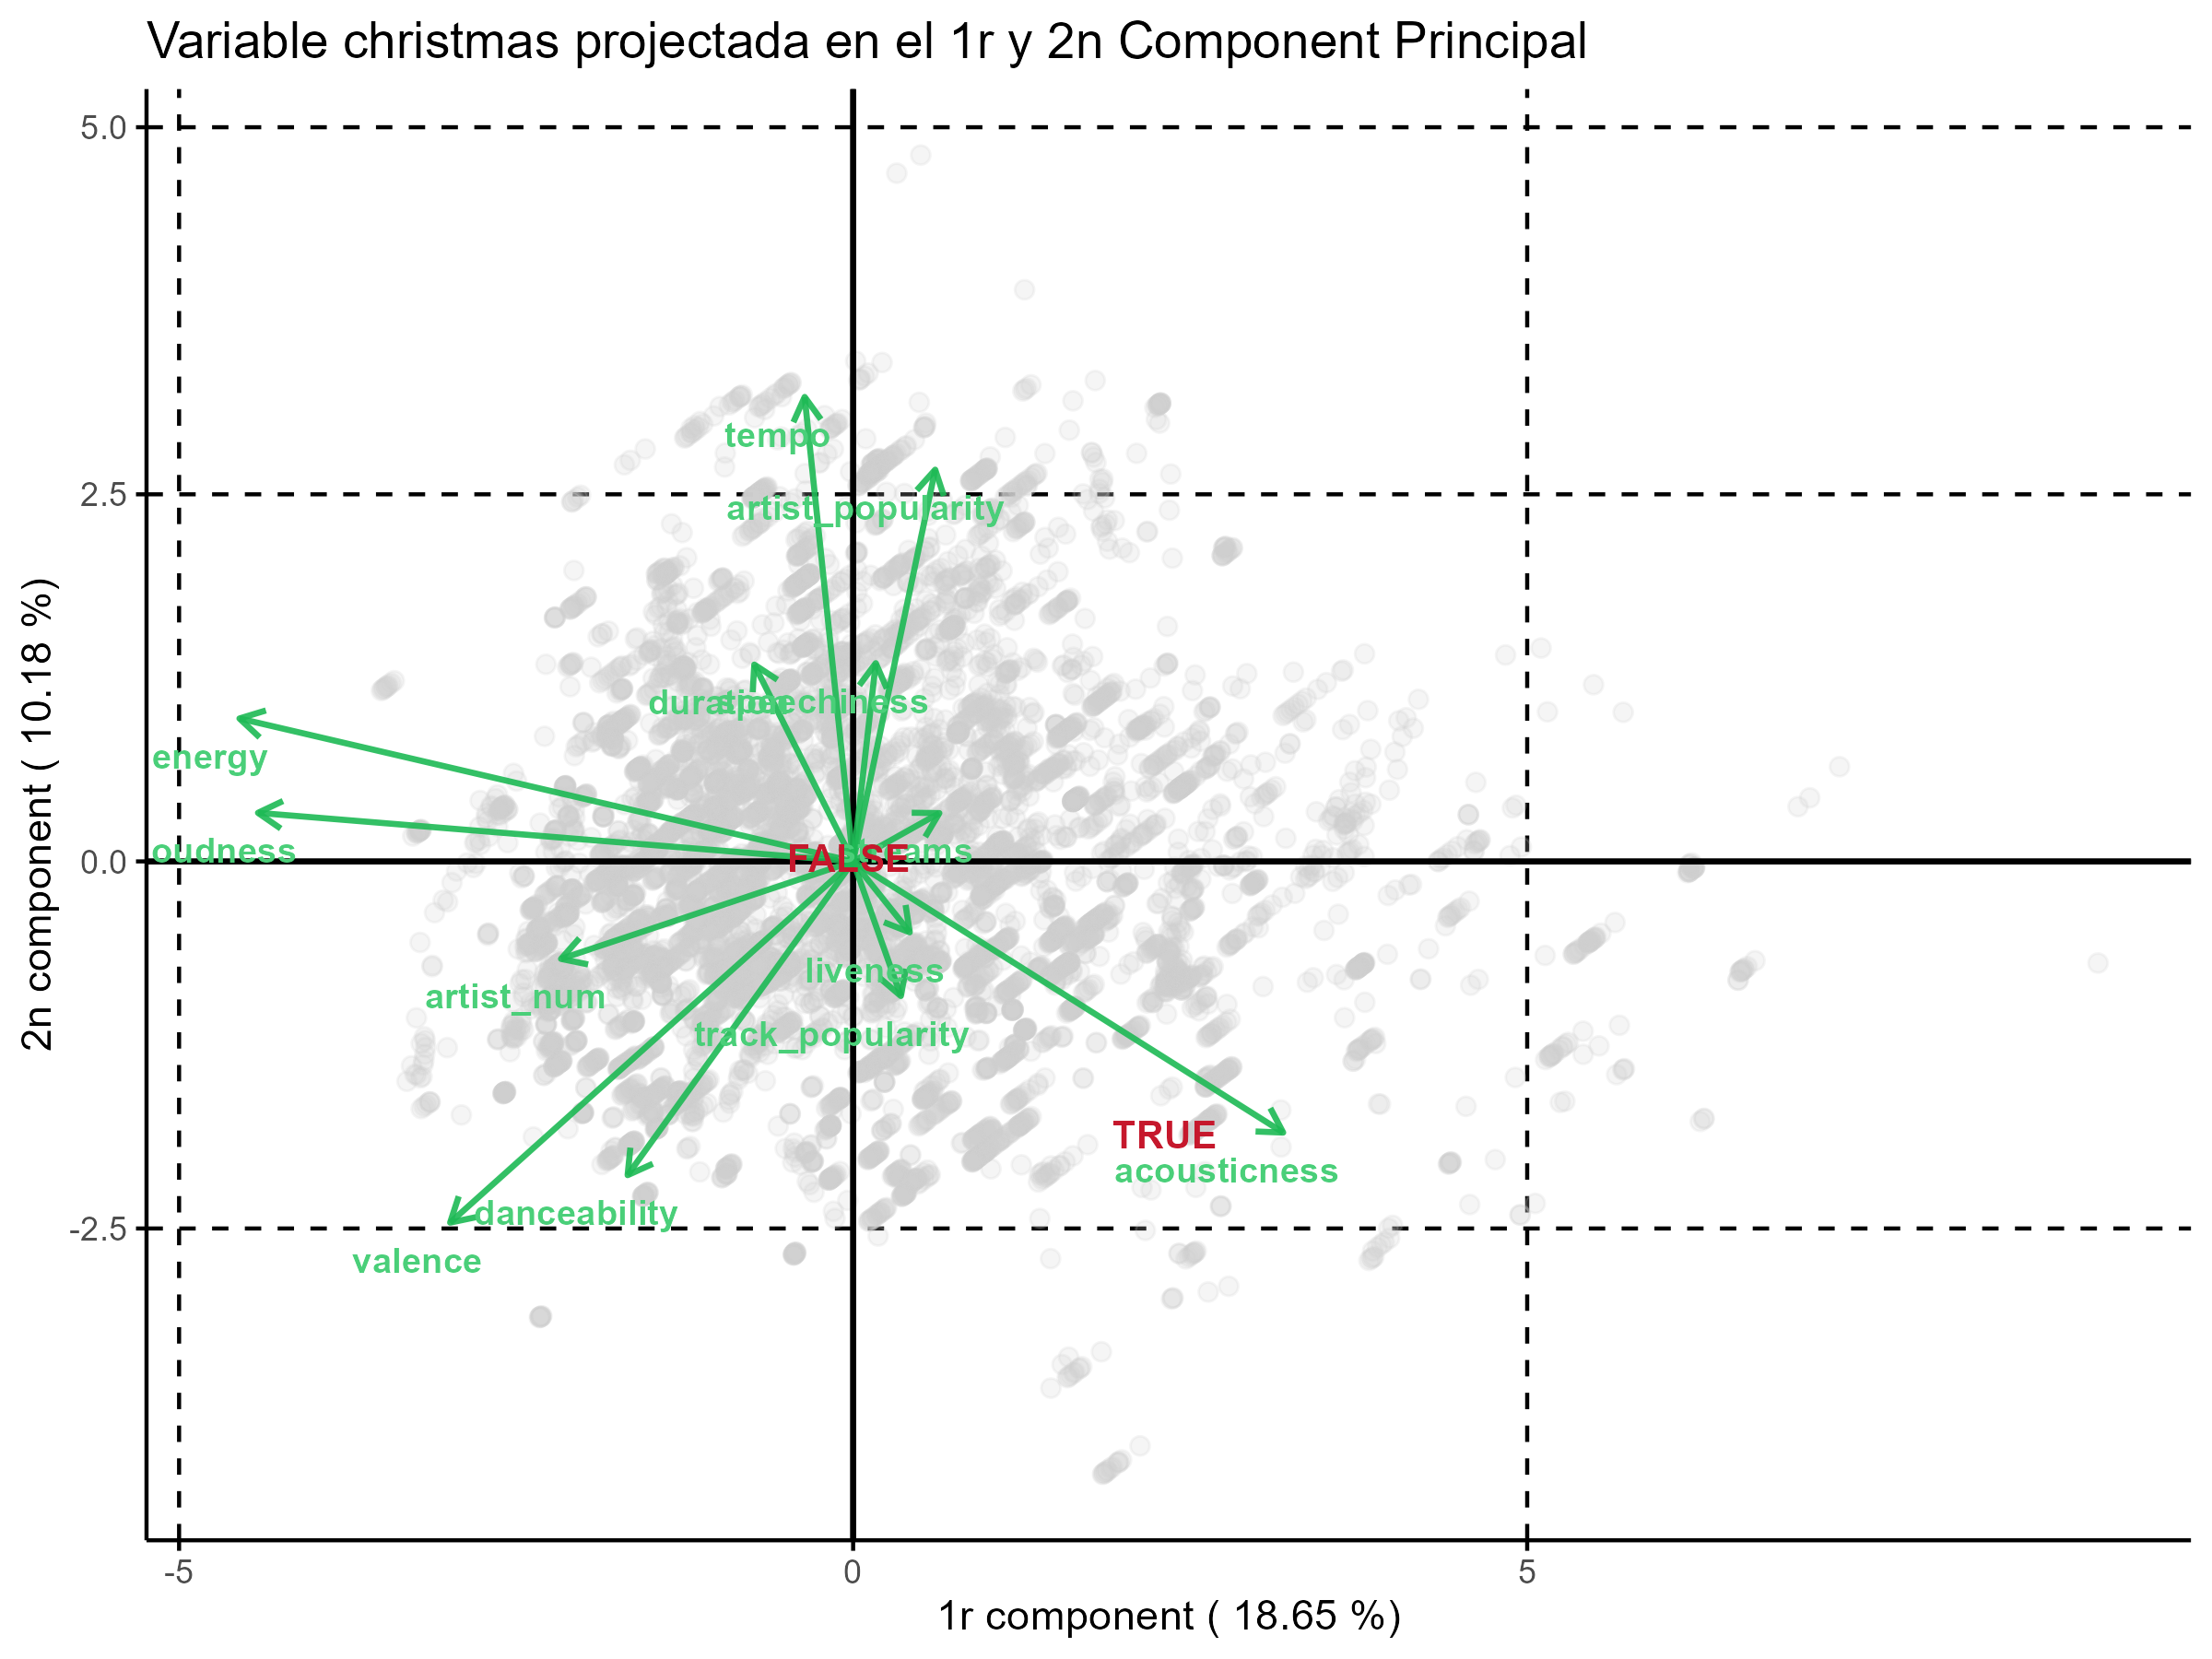
\includegraphics[width=0.6\linewidth]{Images/6_Factorial_Methods/ACP/Cat_C1_C2_christmas.png}
    \caption{Centroides de les classes de la variable christmas projectats en els components 1 i 2}
    \label{fig:6_FM:ACP_christmas}
\end{figure}

La variable nationality té moltes classes i els seus centroides es poden veure projectats en els dos primers components en la figura \ref{fig:6_FM:ACP_nationality}. Es pot destacar els centroides de les classes més propers a valence i danceability són de països d'amèrica llatina (República Dominicana, Venezuela, Mèxic). Això ens indica que els artistes d'aquests països fan cançons generalment més ballables i alegres.

\begin{figure}[H]
    \centering
    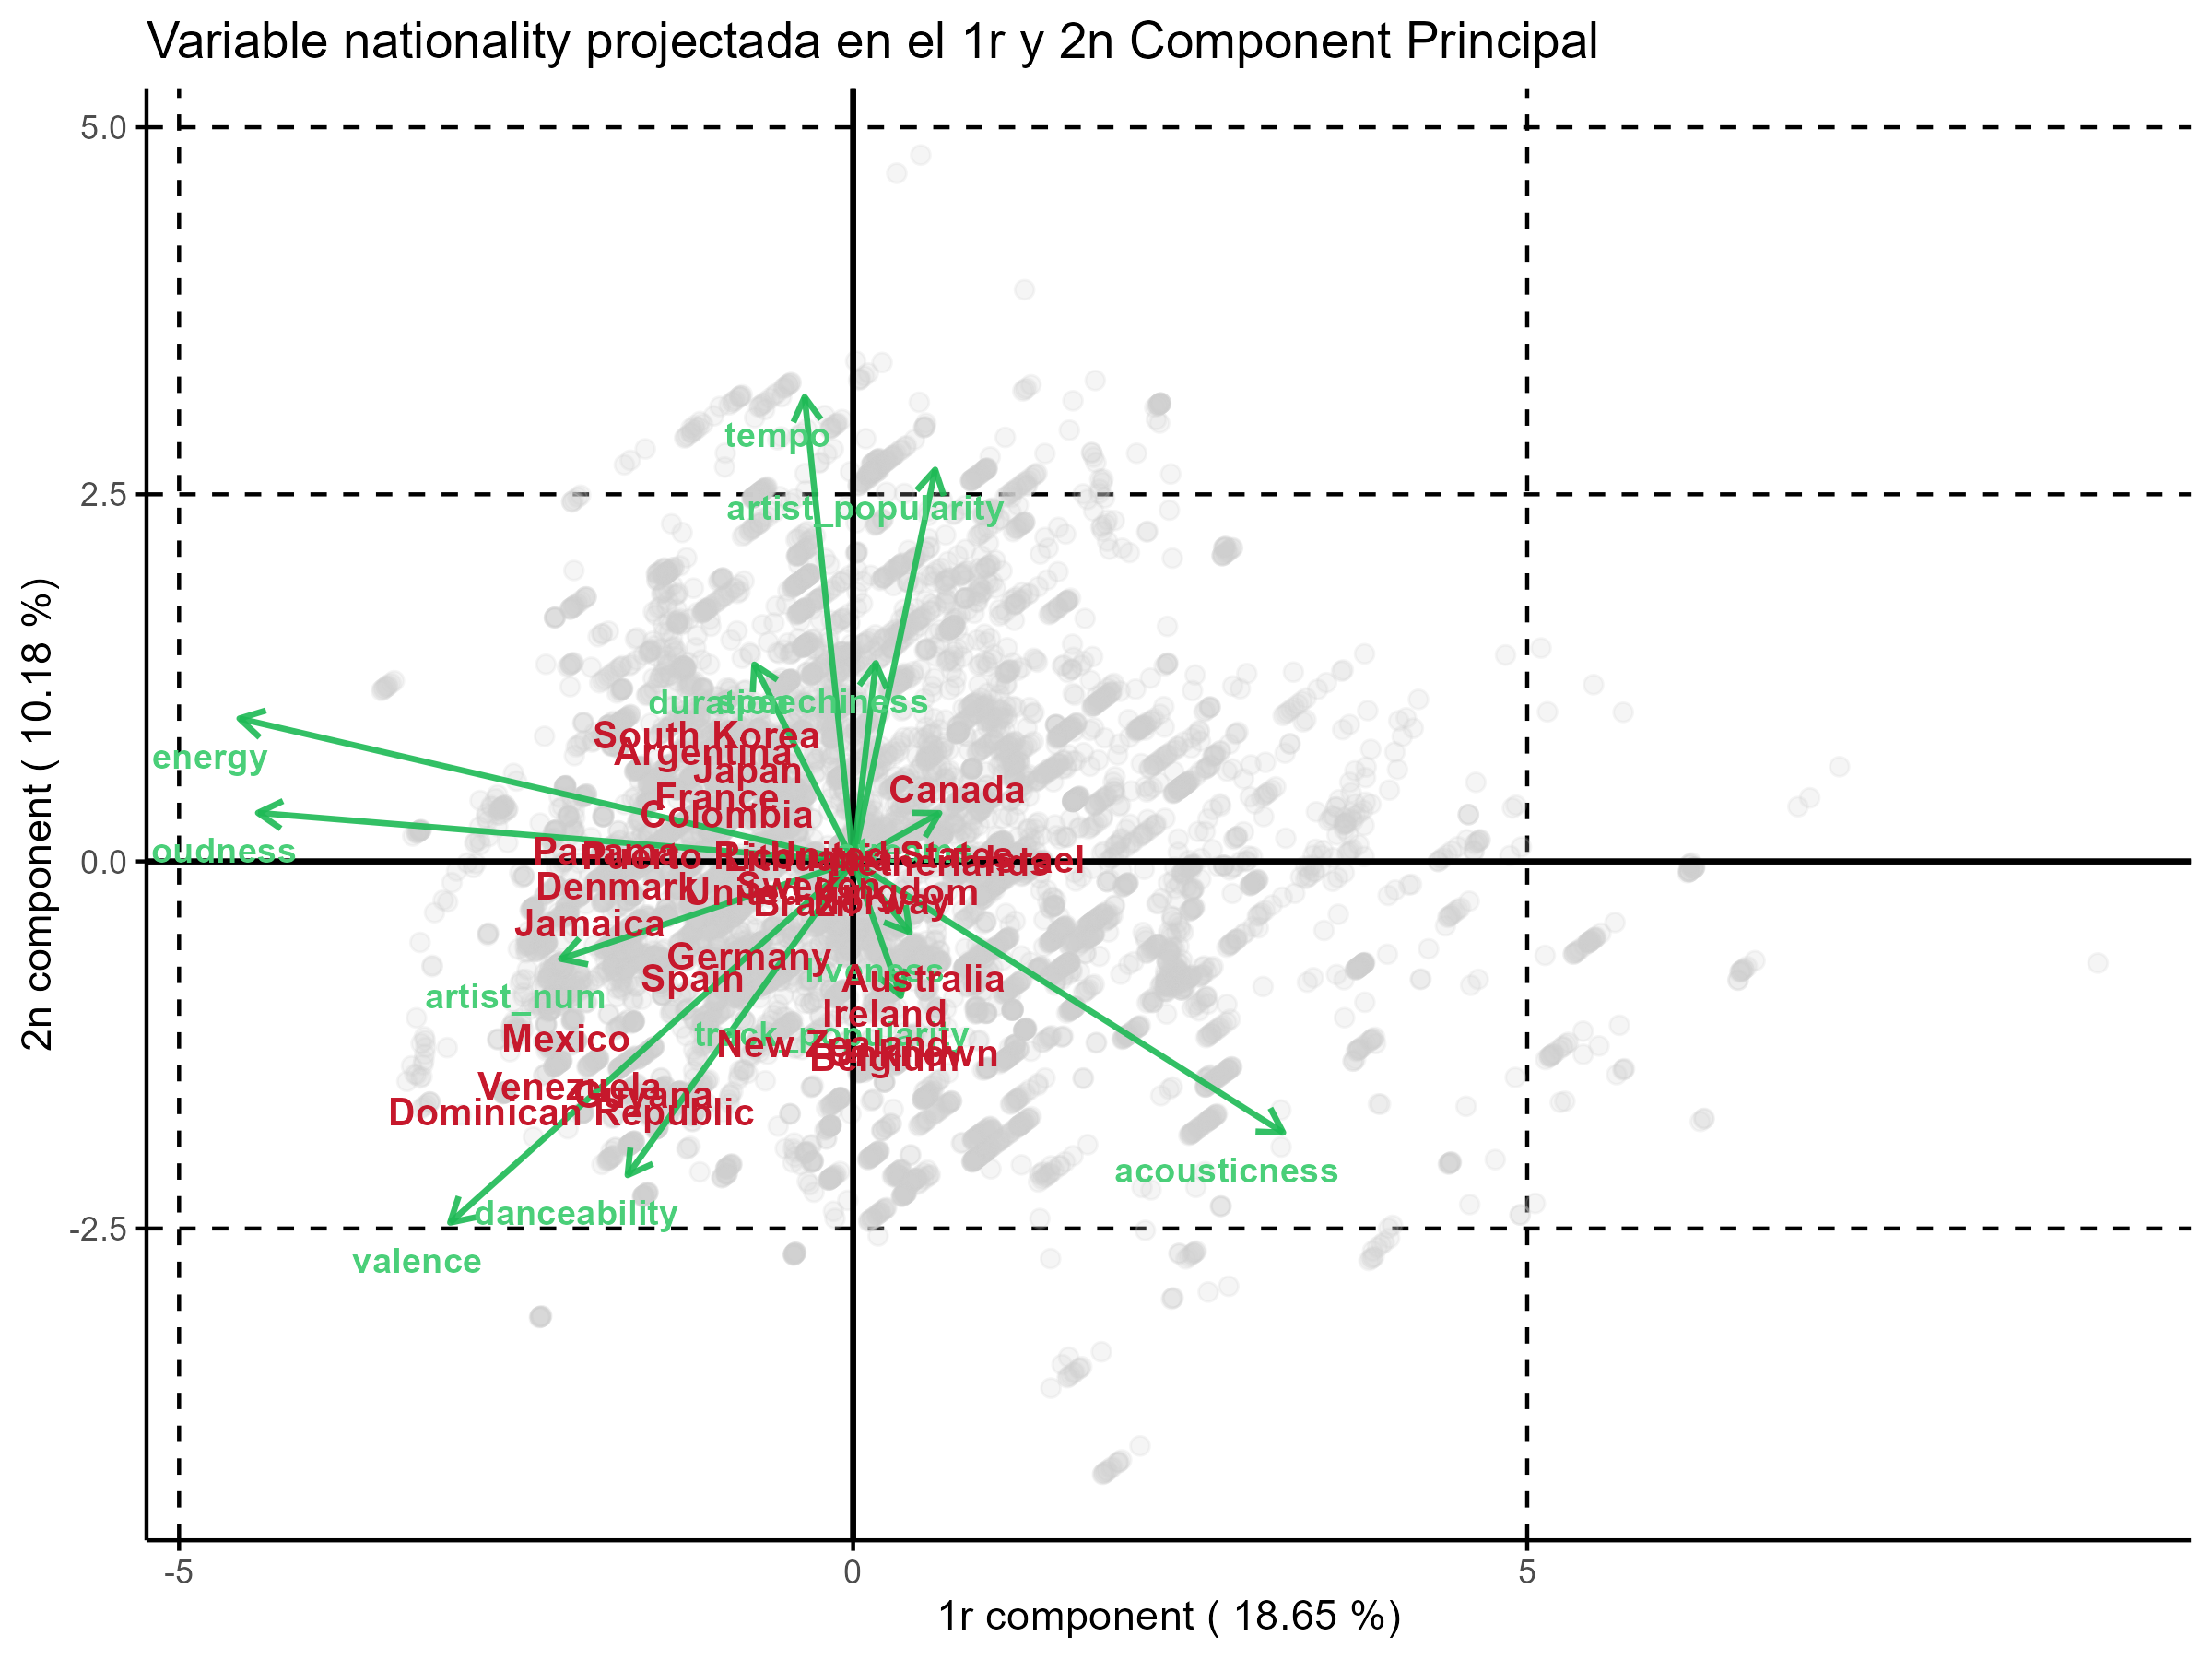
\includegraphics[width=0.6\linewidth]{Images/6_Factorial_Methods/ACP/Cat_C1_C2_nationality.png}
    \caption{Centroides de les classes de la variable nationality projectats en els components 1 i 2}
    \label{fig:6_FM:ACP_nationality}
\end{figure}

Finalment, en la variable time\_signature (compàs), tal i com es pot apreciar en la figura \ref{fig:6_FM:ACP_timesignature}, hi destaca clarament el valor 3 (representant un compàs de 3/4) es troba molt allunyat de la resta de classes. Per la seva projecció en el component1, es pot inferir que es troba en cançons poc energètiques o amb poca ``potència''. Això és coherent amb el fet de que aquest compàs generalment s'utilitza generalment en el gènere de vals, tot i que pot arribar a tenir aparicions en cançons ``tranquiles'' de rock o pop.
\begin{figure}[H]
    \centering
    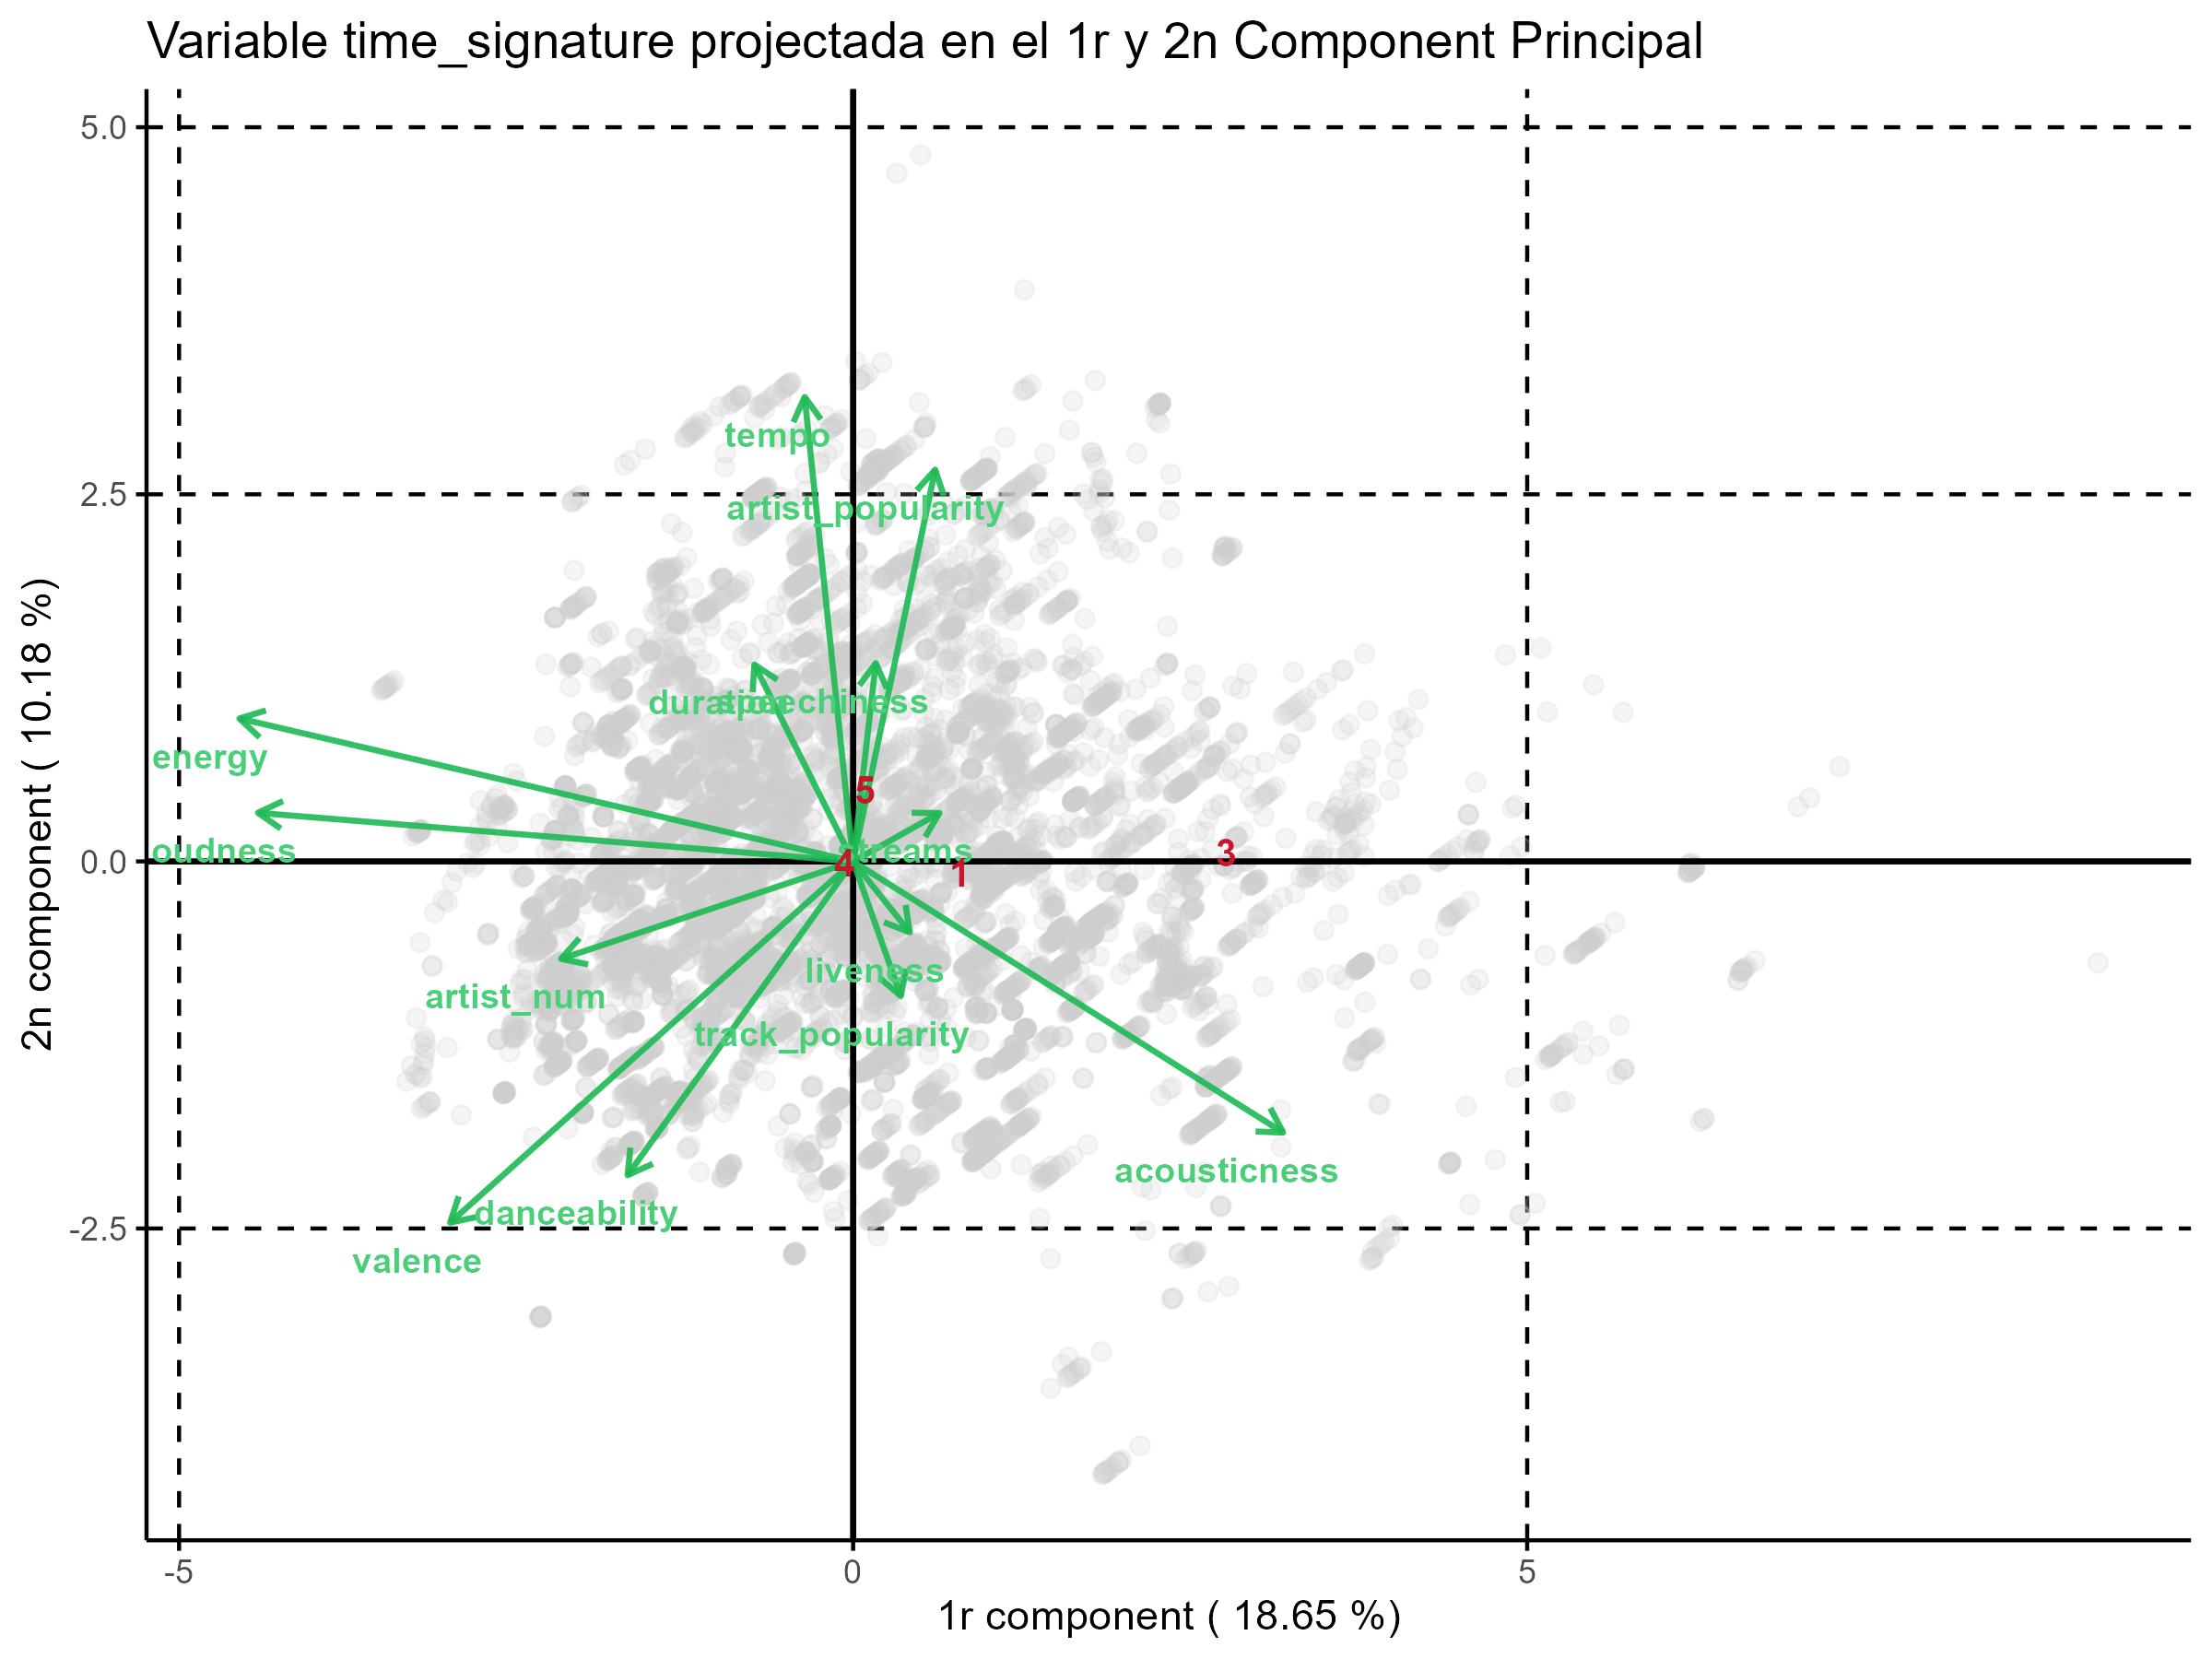
\includegraphics[width=0.6\linewidth]{Images/6_Factorial_Methods/ACP/Cat_C1_C2_time_signature.png}
    \caption{Centroides de les classes de la variable time\_signature projectats en els components 1 i 2}
    \label{fig:6_FM:ACP_timesignature}
\end{figure}

\subsection{Models}
Una vegada es tenen les dades de l'ACM i l'ACP, s'ha creat un model per tal de predir la variable categòrica explicit (que indica si una cançó és explicita o no). Aquest model és una xarxa neuronal creada mitjançant les llibreries \textit{tensorflow} i \textit{keras3} de R. A més, també s'ha afegit un model base (perceptró) per tal de comparar els resultats amb la xarxa neuronal.

\subsection{Preparació de dades}
Per tal de poder entrenar correctament els models, la base de dades utilitzada conté 50 variables numèriques: 9 corresponent als components de l'ACP que expliquen el 80\% de la variància i 41 corresponents a l'ACM que també expliquen un 80\% de la variància.

Per tal de poder entrenar i validar el model correctament, cal separar la base de dades en una partició de train (entrenament) i un de test. A més, també s'utilitzarà una partició de validation per tal de controlar millor l'aprenentatge del model. Com que en la base de dades d'aquest projecte hi ha cançons que es troben en diferents setmanes (és a dir, cançons que apareixen en diferents files en el dataset), les particions de dades s'han hagut de fer per track\_id (identificador únic de cada cançó) en comptes de per files. Pel que fa a les proporicions, la partició de train conté un 80\% de les cançons, mentre que el test conté el 20\% restant. Dins del 80\% de train, el 20\% (16\% del total) s'utilitzarà per la validació, de manera que l'altre 80\% (64\% del total) s'utilitzarà realment per l'entrenament. Cal mencionar que l'opció de realitzar una validació creuada amb k-folds s'ha descartat degut al temps que tarden els models en entrenar-se, ja que augmentarien molt el temps d'entrenament i seria difícil fer suficients proves per determinar quins són els millors paràmetres o arquitectures dels models. Cal mencionar que totes aquestes particions s'han fet amb \textit{stratify}; és a dir, mantenint les distribucions de valors en les classes de la variable objectiu en totes les particions per tal de poder entrenar i validar el model amb més robustesa.

Una vegada es tenen totes les particions, s'ha observat que en la partició de train hi havia un desbalanç en la variable objectiu. Concretament, en la variable explicit s'hi troben 3466 valors de la classe 0 (FALSE, cançó no explícita) i 2116 de classe 1 (TRUE, cançó explicita). Aquest desbalanç pot acabar generant underfitting i mals resultats dels models. Per tant, per compensar aquest problema s'han provat diferents solucions:
\begin{enumerate}
    \item \textbf{Random oversampling}: Aquest mètode consisteix en duplicar files de la base de dades aleatòriament i de la classe minoritària fins que la quantitat de mostres de totes dues classes s'hagi igualat. Sovint porta a overfitting, ja que conté dades repetides.

    \item \textbf{Random undersampling}: Aquest mètode consisteix en eliminar files de la base de dades aleatòriament i de la classe majoritària fins que la quantitat de mostres de totes dues classes s'hagi igualat. Sovint porta a underfitting, ja que elimina dades de la partició d'entrenament.

    \item \textbf{Weights}: Aquest mètode assigna ``pesos'' (weights) a totes les mostres de la base de dades, donant més pes a les que són de la classe minoritària i menys pes a les de la classe majoritària. Aquest mètode permet no perdre informació de les dades d'entrenament i fa que el model aprengui més amb les dades de la classe minoritària (ja que n'hi ha menys). Aquests pesos es calculen automàticament en funció del nombre d'individus de cada classe per tal de que l'aprenentatge sigui similar en tots dos casos.

    \item \textbf{SMOTE}: Synthetic Minority Oversampling TEchnique és un mètode d'oversampling que considera aleatòriament un dels k veïns d'un individu per tal de crear una nova dada sintètica amb valors que oscil·lin entre els que té l'individu i els que té el veí seleccionat. Això es fa, evidentment, per la classe minoritària fins que s'aconsegueix que estiguin balancejades. Generalment aconsegueix generar dades sintètiques de bona qualitat i permet que els models aprenguin millor.
\end{enumerate}

Aquests mètodes s'han provat i s'ha arribat a la conclusió de que els millors són weights i SMOTE, i el que s'ha acabat utilitzant ha sigut weights, ja que així no s'introdueixen dades sintètiques en la base de dades.

\subsubsection{Model base}
Per al model base s'ha utilitzat un perceptró. Com que es vol realitzar una classificació binària (explicit TRUE o FALSE), el perceptró serà una sola neurona amb funció d'activació sigmoide, que permet obtenir les probabilitats de pertànyer a la classe positiva o a la negativa. Amb aquesta arquitectura, el perceptró té la mateixa estructura que una Regressió Logística i servirà com a model base.

El batch size, optimitzador, learning rate i early stopping utilitzats durant l'entrenament seran sempre els mateixos que per la xarxa neuronal.

\subsubsection{Model avançat}
Aquest model és una xarxa neuronal que s'ha provat amb múltiples paràmetres fins donar amb els que sembla que millor rendiment tenen. 

Per començar, s'ha utilitzat un batch size de 8, de manera que en cada iteració de l'entrenament el model considera només 8 files del dataset. 

L'optimitzador utilitzat ha estat ADAM, ja que generalment és el que proporciona millor rendiment i convergència més ràpida. El learning rate utilitzat s'ha provat amb diferents valors fixes, però finalment s'ha optat per un valor dinàmic, que comença a 0.005 i es redueix un 10\% cada 10000 passos.

Pel que fa al nombre d'epochs, s'ha establert a 100, però s'ha definit un mètode de early stopping per aturar l'entrenament quan l'error de validació no millori més. El paràmetre ``patience'' (nombre d'iteracions en les que es segueix entrenant encara que l'error de validació no millori) s'ha establert a 10.

Per altra banda, s'ha provat amb diferents funcions d'activació per les capes ocultes de la xarxa (ja que la de la sortida ha de ser una sigmoide degut que es tracta d'una classificació binària) i s'ha determinat que la ReLU i la TanH (Tangent Hiperbòlica) són les que millor rendeixen. S'ha escollit TanH ja que generalment ha proporcionat millors resultats.

Com ja s'ha dit, tots aquests paràmetres mencionats també s'utilitzen pel model base per tal de que es puguin comparar millor.

Finalment, pel que fa a l'arquitectura de la xarxa, s'han afegit 3 capes ocultes, amb 128, 128 i 64 neurones, respectivament. A més, després de cada una de les capes ocultes, s'ha afegit una capa de regularització de l'activitat (activity regularization). Aquesta regularització penalitza l'alta activació de neurones, controlant així l'overfitting del model i fent que sigui més robust. Concretament, s'ha establert amb coeficient 0.001 a la penalització de tipus L2, que penalitza proporcionalment al quadrat de la magnitud de les activacions de neurones.

\subsubsection{Resultats}
Abans de res, cal mencionar que els resultats varien lleugerament depenent de l'execució (encara que es fixi una llavor). No obstant, els valors que es mostren a continuació són bastant comuns després d'haver realitzat múltiples execucions.

A més, cal remarcar que la principal mètrica que s'ha utilitzat per avaluar els models és l'F1-Score, i no pas l'accuracy; ja que, com s'ha mencionat anteriorment, les classes de la variable objectiu estan desbalancejades i si es tingués en compte l'accuracy es podria arribar a un model que fa underfit i simplement tendeix a predir la classe majoritària.

En el model base els resultats han estat molt bons, amb F1-Score de 0.7685, accuracy de 0.8172,  precision de 0.8117, recall de 0.7297 i la matriu de confussió que es pot veure en la figura \ref{fig:6_FM:NN_cm_perc}. A més, en les figures \ref{fig:6_FM:NN_loss_perc} i \ref{fig:6_FM:NN_acc_perc} es poden veure l'evolució de l'accuracy i de la loss (error) al llarg de les epochs de l'entrenament, tant per la partició de train com per la de validation. Es pot apreciar que en la partició de validation augmenta l'error a mesura que augmenten les epochs, però això no ens ha de preocupar excessivament ja que l'early stopping recupera els pesos de la iteració amb menys error en la validació.

\begin{figure}[H]
    \centering
    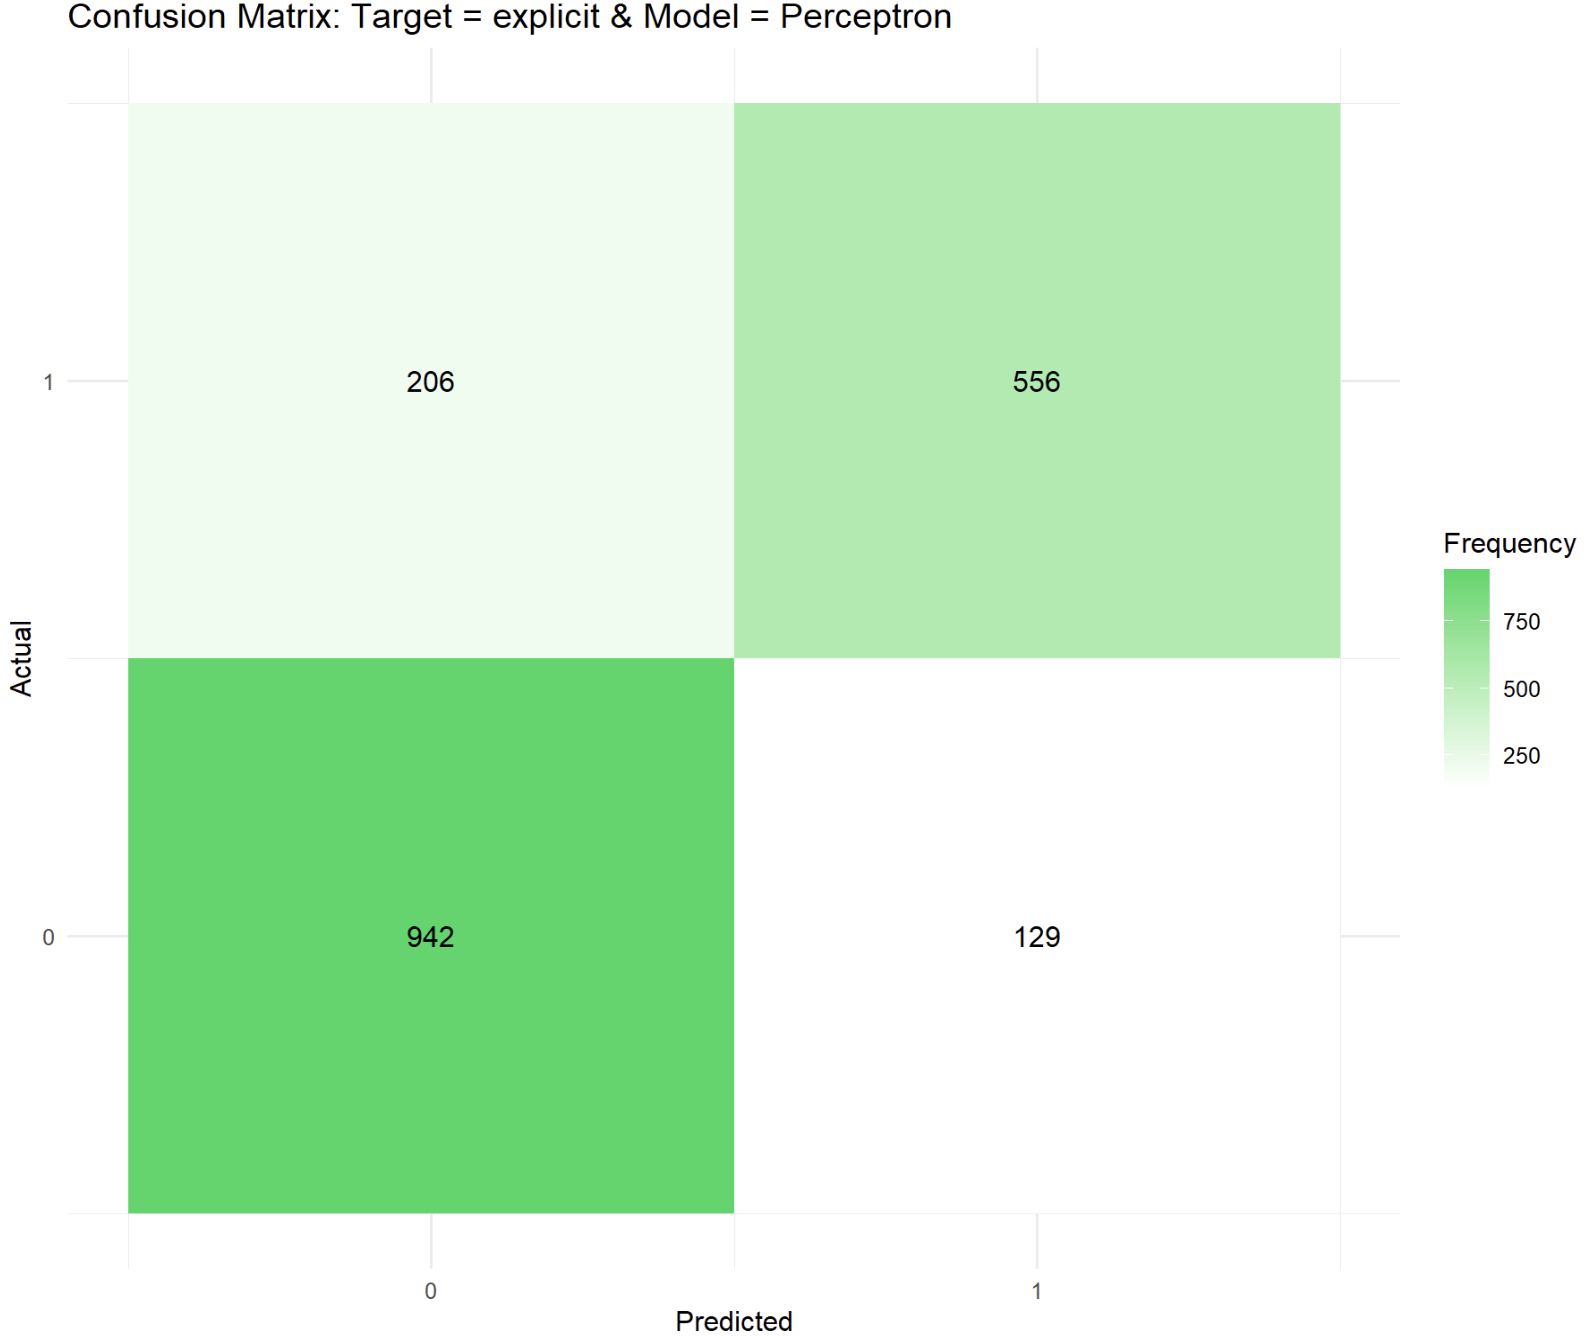
\includegraphics[width=0.8\linewidth]{Images/6_Factorial_Methods/NN/cm_perc.png}
    \caption{Matriu de confusió del model base}
    \label{fig:6_FM:NN_cm_perc}
\end{figure}

\begin{figure}[H]
    \centering
    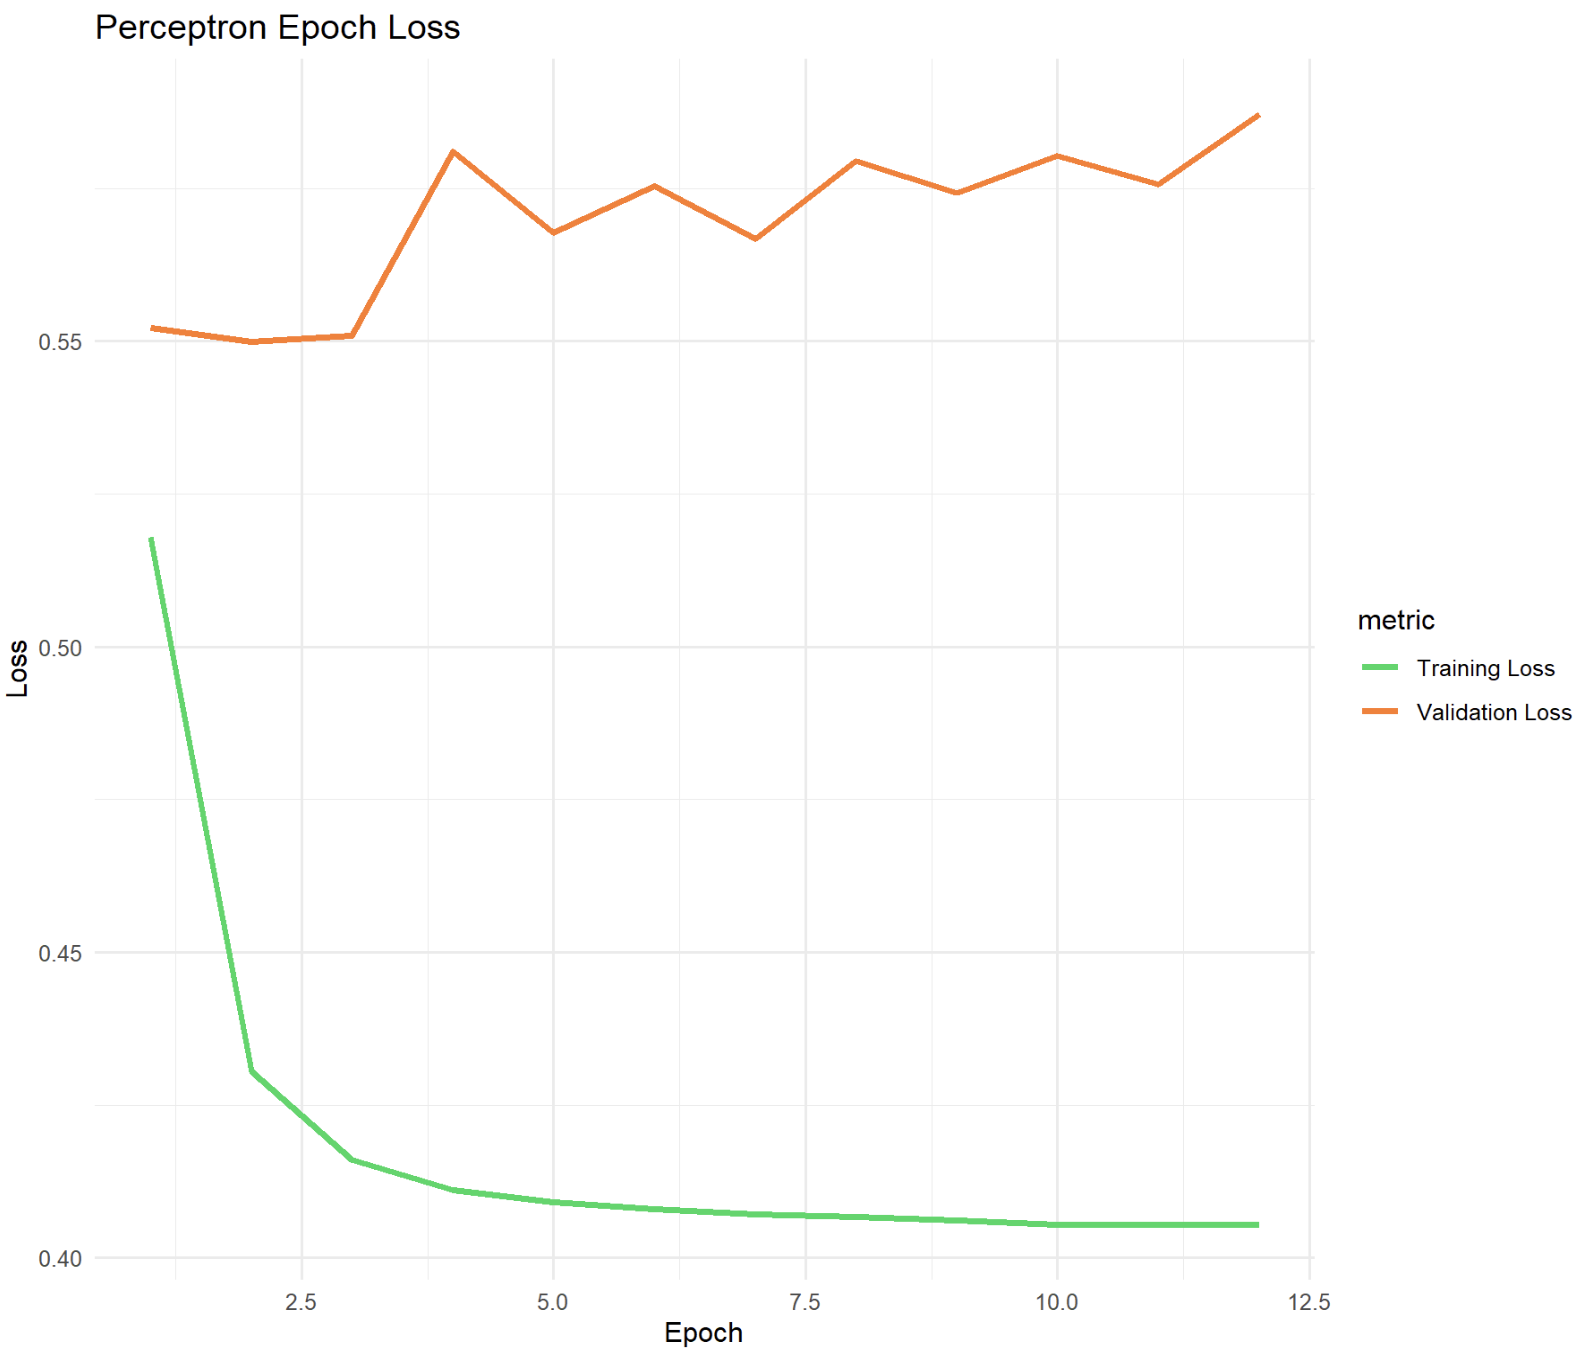
\includegraphics[width=0.65\linewidth]{Images/6_Factorial_Methods/NN/loss_perc.png}
    \caption{Evolució de l'error de train i validation en funció de les epochs del model base}
    \label{fig:6_FM:NN_loss_perc}
\end{figure}

\begin{figure}[H]
    \centering
    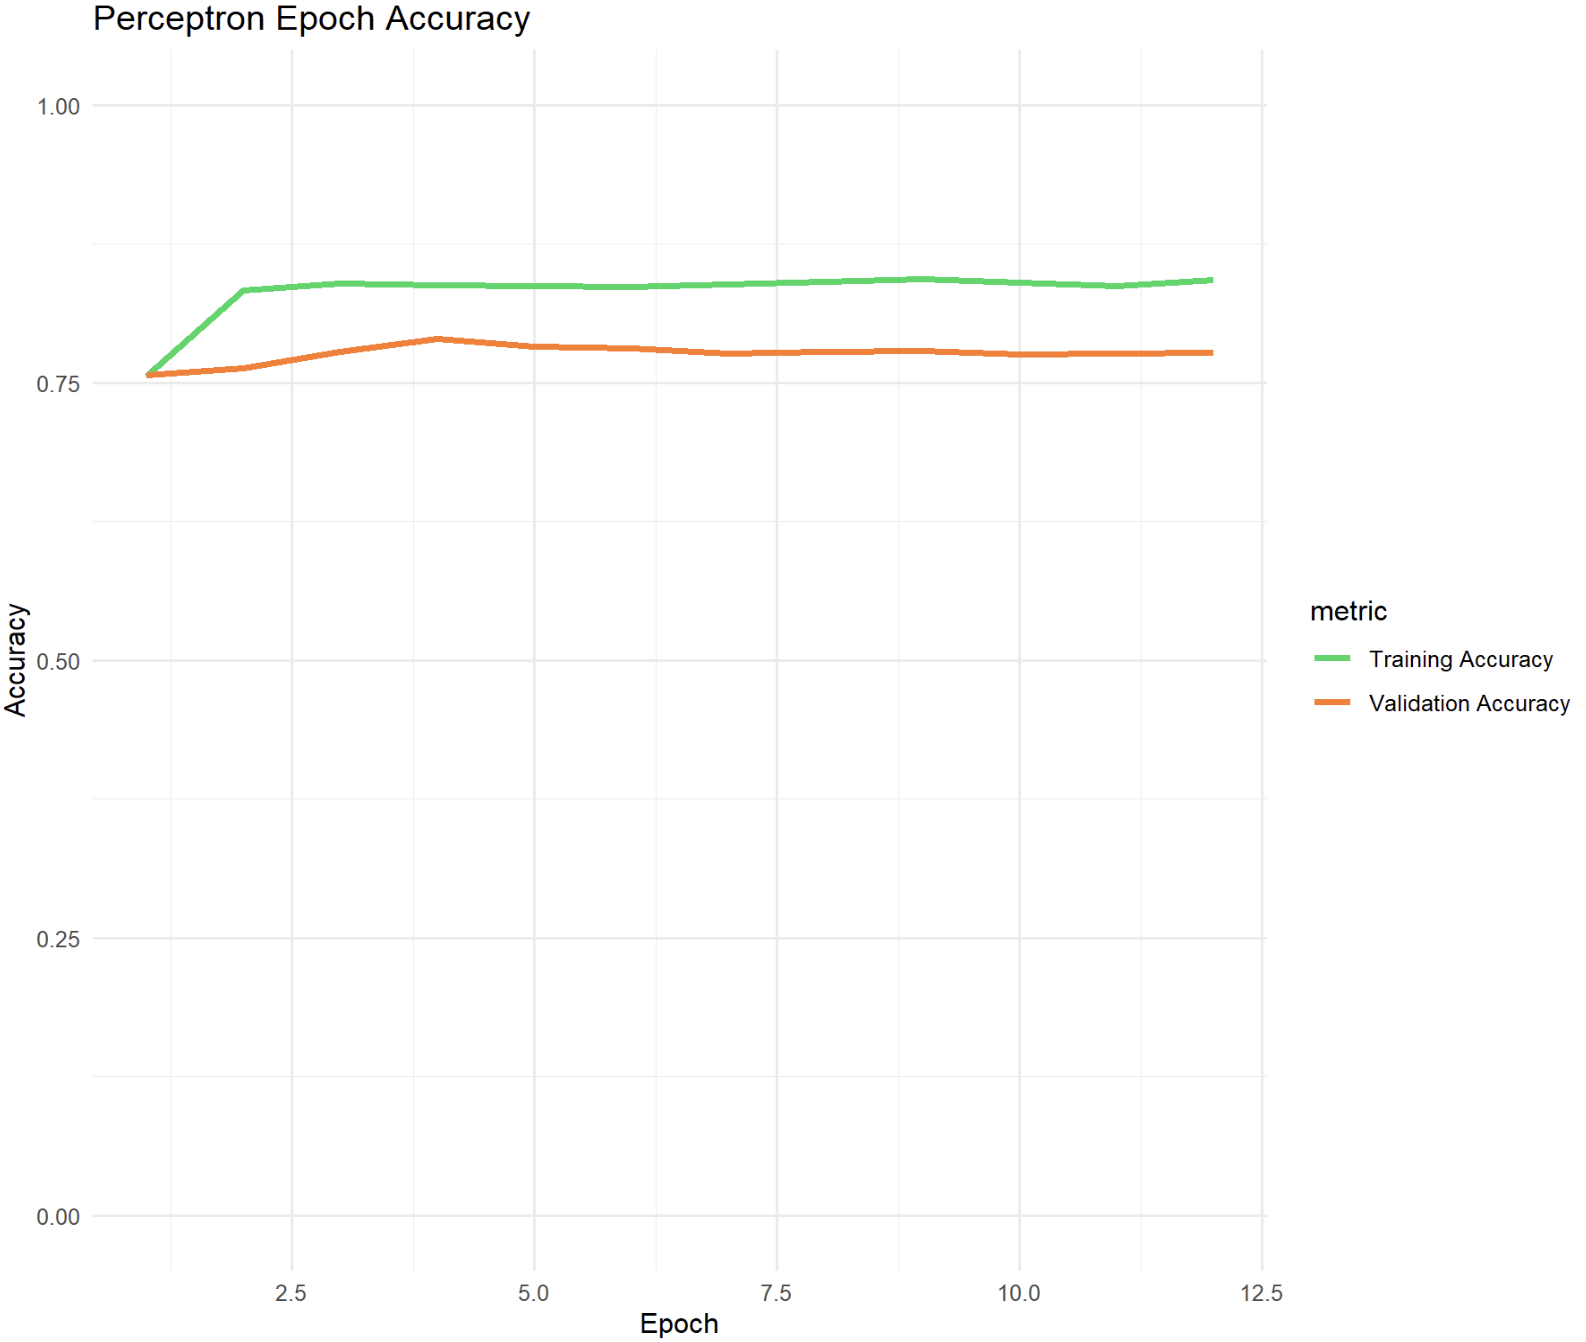
\includegraphics[width=0.65\linewidth]{Images/6_Factorial_Methods/NN/acc_perc.png}
    \caption{Evolució de l'accuracy de train i validation en funció de les epochs del model base}
    \label{fig:6_FM:NN_acc_perc}
\end{figure}

Per altra banda, en el model avançat (xarxa neuronal) els resultats han estat molt bons, amb F1-Score de 0.7698, accuracy de 0.8238,  precision de 0.8424, recall de 0.7087 i la matriu de confussió que es pot veure en la figura \ref{fig:6_FM:NN_cm_mlp}. A més, en les figures \ref{fig:6_FM:NN_loss_mlp} i \ref{fig:6_FM:NN_acc_mlp} es poden veure l'evolució de l'accuracy i de la loss (error) al llarg de les epochs de l'entrenament, tant per la partició de train com per la de validation. Es pot apreciar que en la partició de validation augmenta l'error a mesura que augmenten les epochs, però això no ens ha de preocupar excessivament ja que l'early stopping recupera els pesos de la iteració amb menys error en la validació.

\begin{figure}[H]
    \centering
    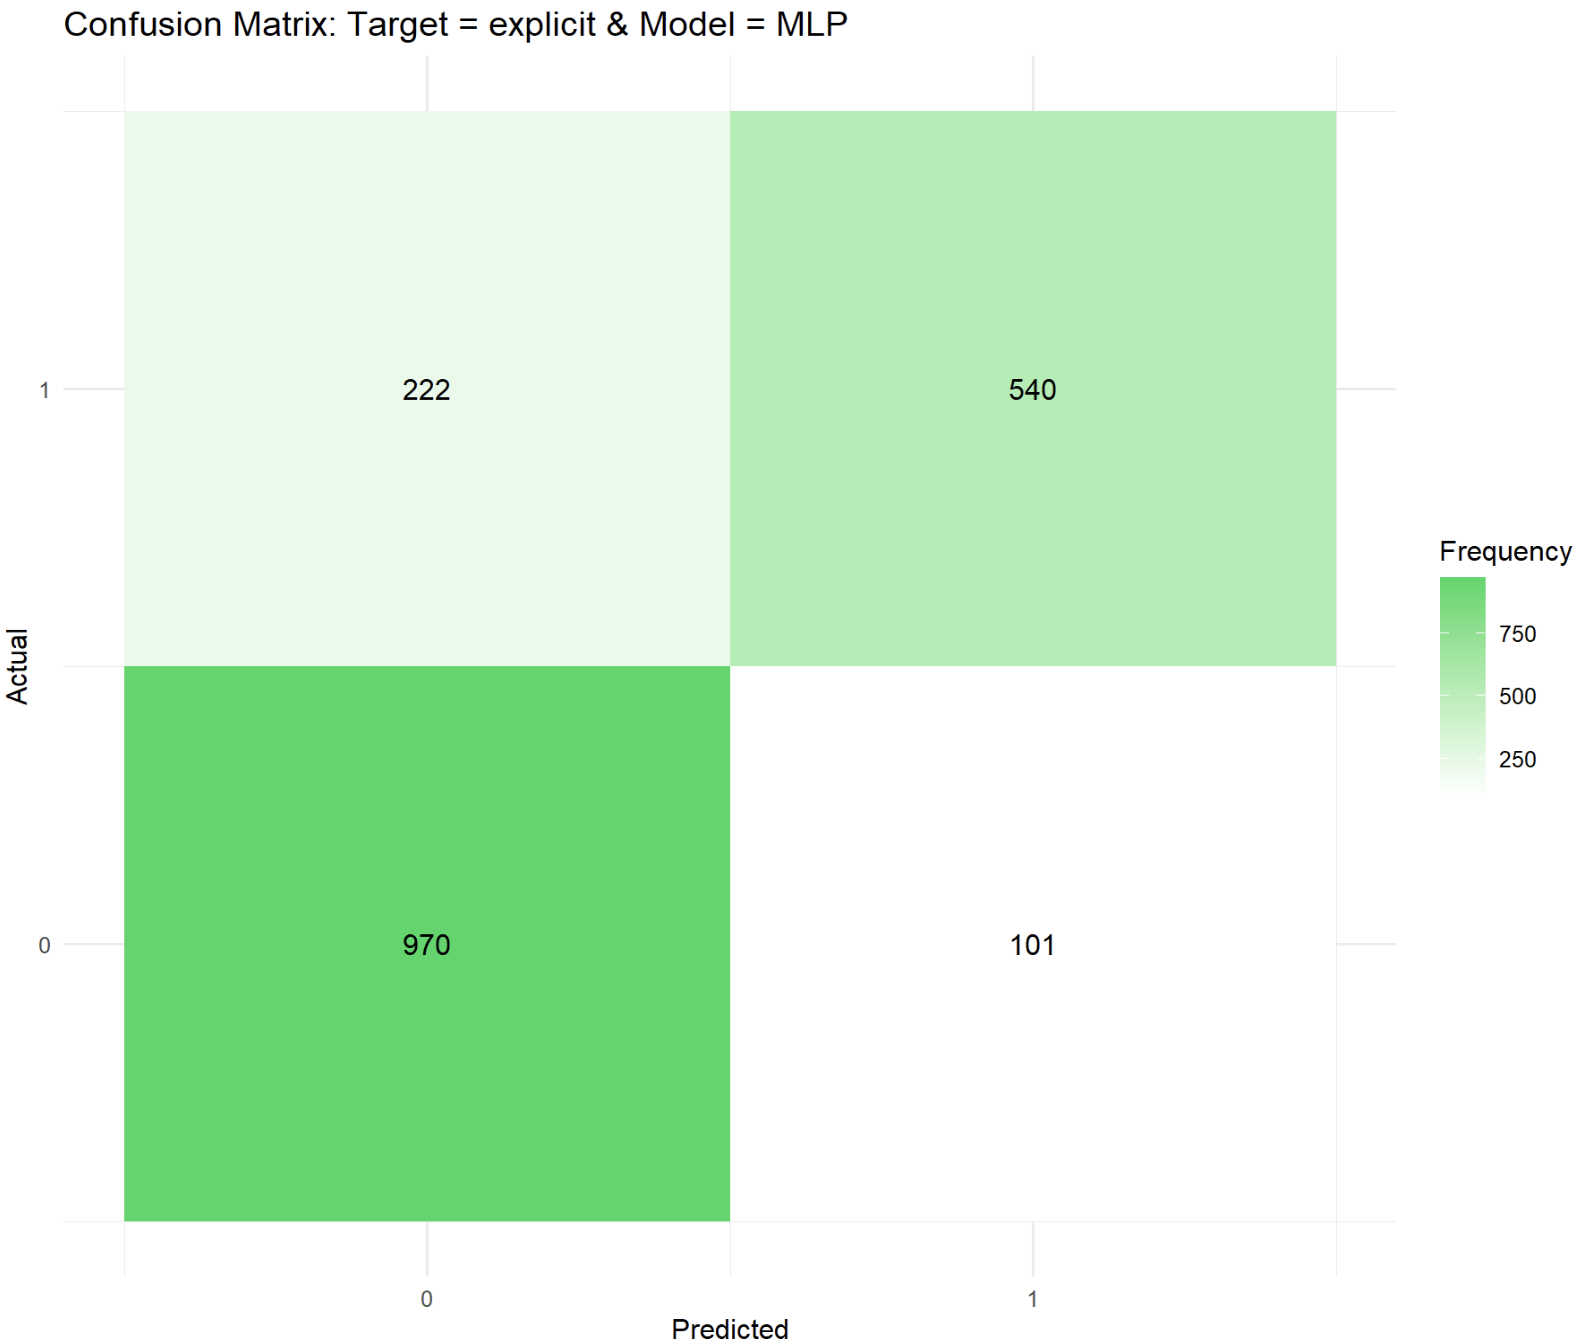
\includegraphics[width=0.8\linewidth]{Images/6_Factorial_Methods/NN/cm_mlp.png}
    \caption{Matriu de confusió del model avançat}
    \label{fig:6_FM:NN_cm_mlp}
\end{figure}

\begin{figure}[H]
    \centering
    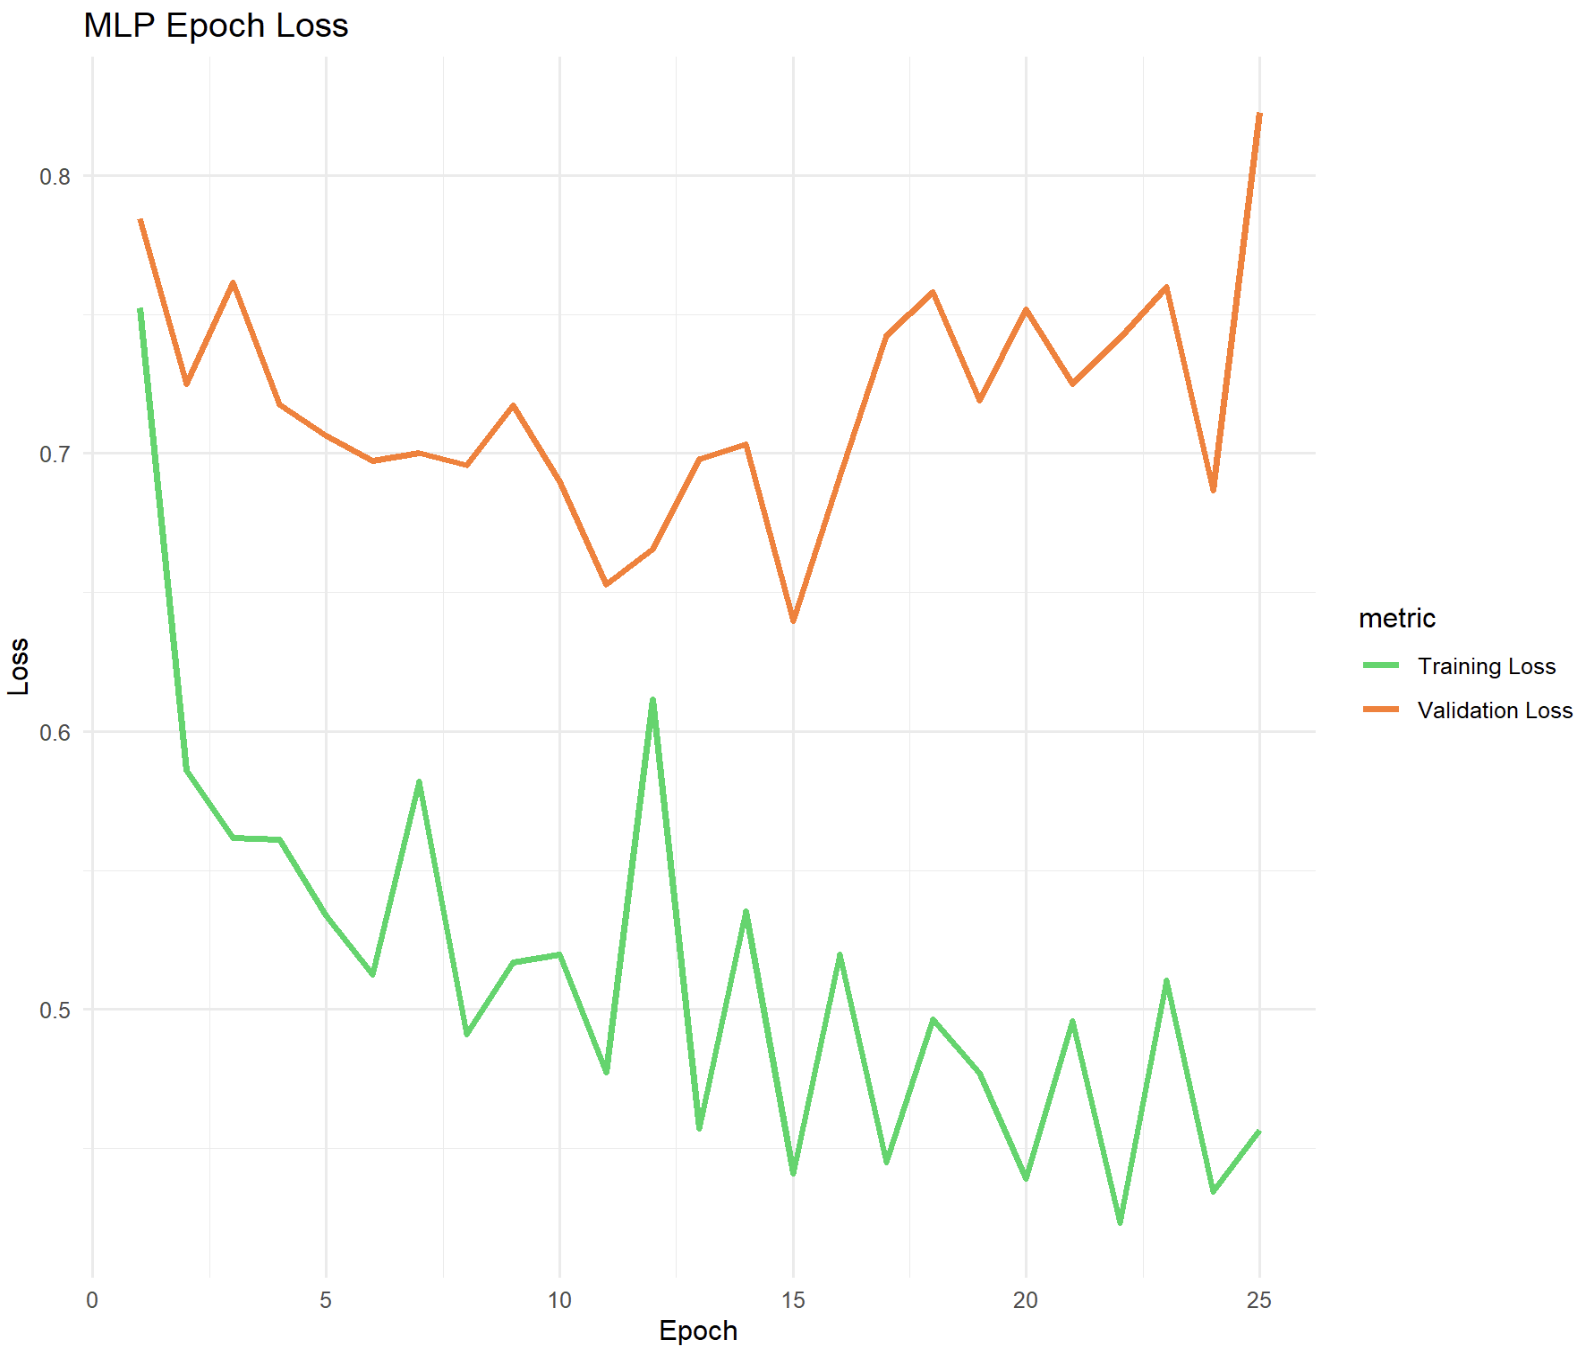
\includegraphics[width=0.65\linewidth]{Images/6_Factorial_Methods/NN/loss_mlp.png}
    \caption{Evolució de l'error de train i validation en funció de les epochs del model avançat}
    \label{fig:6_FM:NN_loss_mlp}
\end{figure}

\begin{figure}[H]
    \centering
    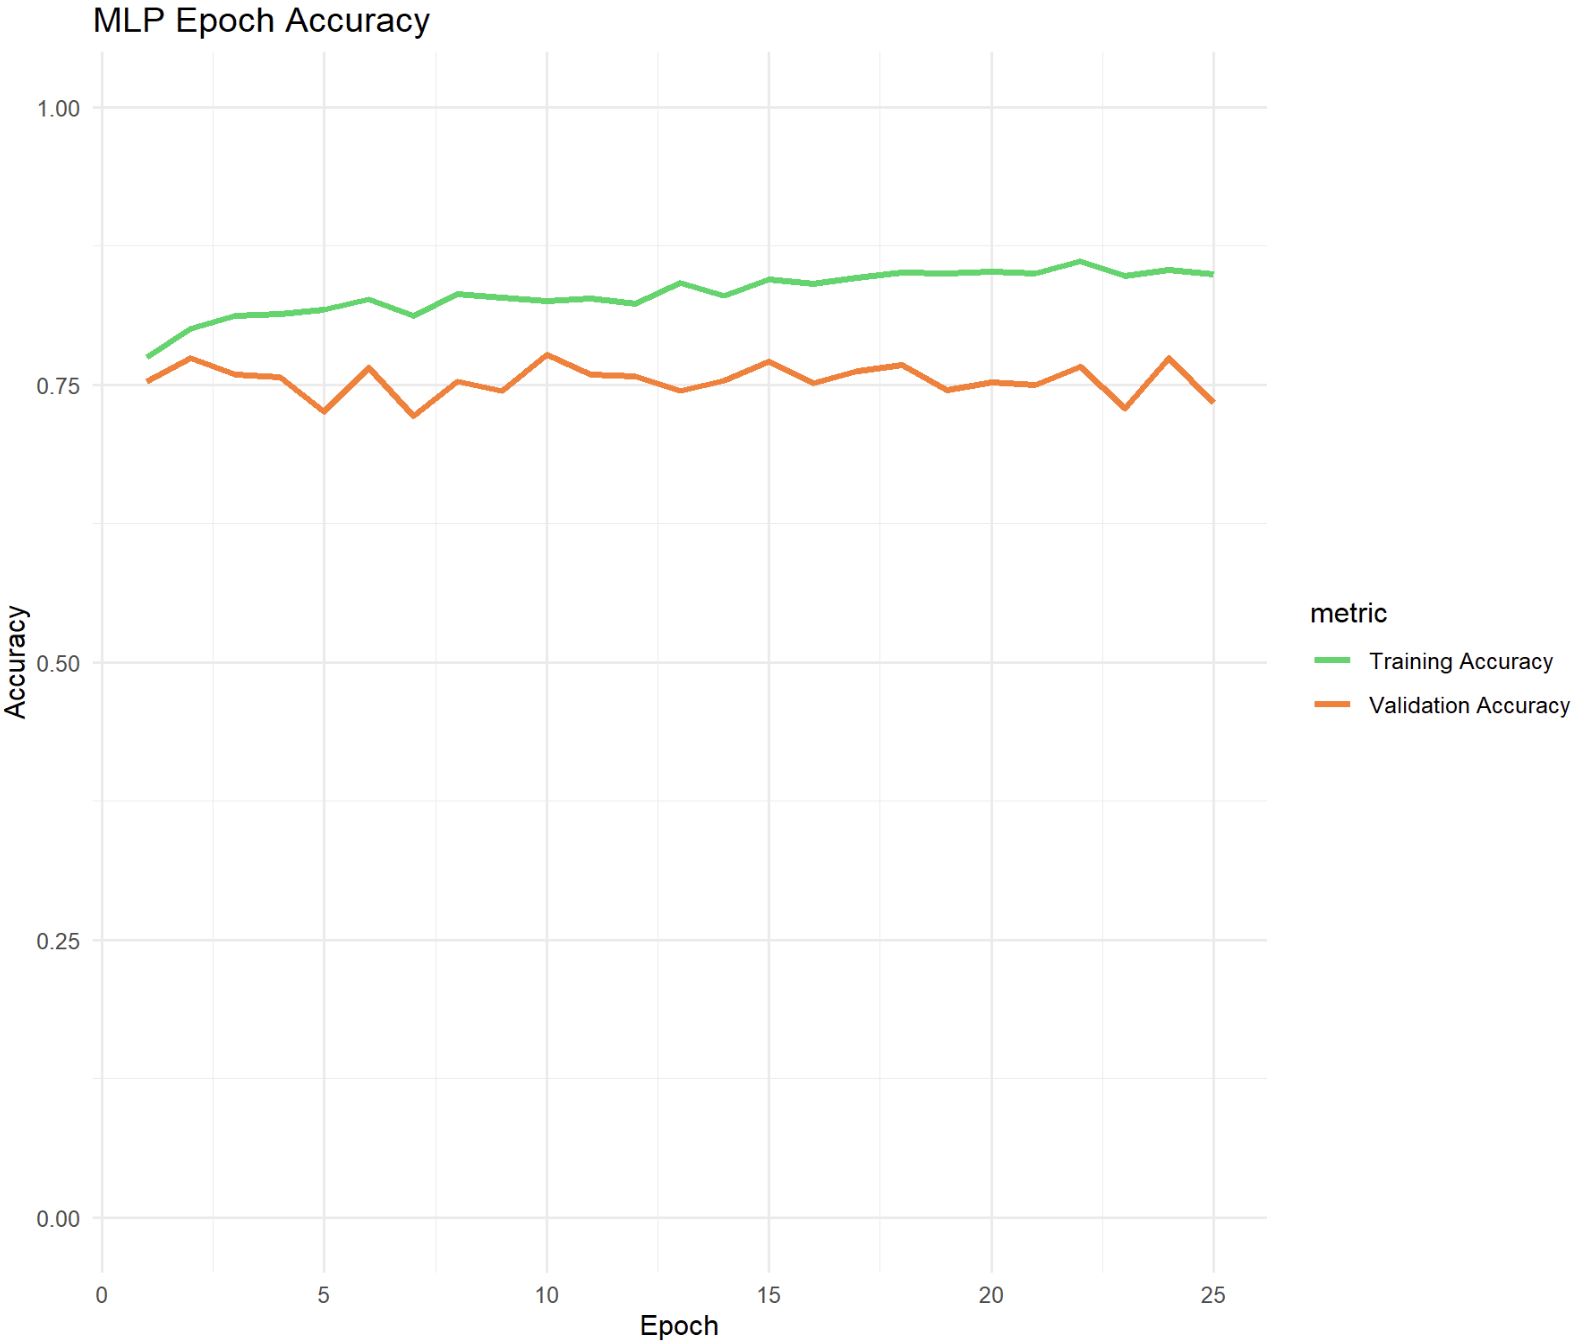
\includegraphics[width=0.65\linewidth]{Images/6_Factorial_Methods/NN/acc_mlp.png}
    \caption{Evolució de l'accuracy de train i validation en funció de les epochs del model avançat}
    \label{fig:6_FM:NN_acc_mlp}
\end{figure}

Finalment, en la taula \ref{tab:6_FM:NN_metriques} es pot veure el resum de les mètriques mencionades. 

\begin{table}[H]
    \centering
    \begin{tabular}{lrr}
        \toprule
        \textbf{Mètrica} & \textbf{Model Base} & \textbf{Model Avançat} \\
        \midrule
        \textbf{F1-Score} & 0.7685 & 0.7698 \\
        \textbf{Accuracy} & 0.8172 & 0.8238 \\
        \textbf{Precision} & 0.8117 & 0.8424 \\
        \textbf{Recall} & 0.7297 & 0.7087 \\
        \bottomrule
    \end{tabular}
    \caption{Resum de les mètriques obtingudes en els dos models}
    \label{tab:6_FM:NN_metriques}
\end{table}

Com s'ha pogut veure, tot i haver provar moltes combinacions de paràmetres i arquitectures diferents, els resultats són molt similars per tots dos models, de manera que no ha resultat eficaç entrenar un model més avançat que el base. En aquesta execució, el model avançat ha obtingut un F1-Score, Accuracy i Precision molt lleugerament superior al model base, mentre que el model base ha guanyat en Recall. 

Tenint en compte la predicció que s'està fent (predir si una cançó és explicita), és preferible que el model tendeixi a predir que les cançons són explícites, ja que així es podria evitar, per exemple, que nens escoltin cançons explícites a Spotify o altres possibles problemes derivats de no predir correctament la classe positiva. Per tant, la mètrica de Recall és molt important per la predicció que es vol fer, ja que determina la proporció de Veritables Positius que s'han predit correctament respecte el total de Positius reals de la base de dades. En aquest cas, el model base seria lleugerament millor.



           
                                      